\documentclass[12pt]{article}
\markboth{ {\today}}{{\today}}
\pagestyle{myheadings}
\usepackage{amsmath}
\usepackage{epsfig}
 
\begin{document}
 
 
   
   
\newpage 
\setcounter{page}{ 
    26001 } 
   
   
   
   
\noindent\begin{tabular}{|l|}
\hline
YOUR NAME (FIRST, ... LAST)  \\
\hline
 \\ 
 \\ 
\hline
\end{tabular}
\hspace{0.05in} \begin{tabular}{|l|}
\hline
 YOUR   ID   INFORMATION  \\
\hline
 \\ 
 \\ 
\hline
\end{tabular}
   
   
\vspace{0.2in}\noindent\begin{tabular}{|l|}
\hline
YOUR TOTAL MARKS  \\
\hline
 \\ 
 \\ 
\hline
\end{tabular}
\hspace{0.05in} \begin{tabular}{|l|}
\hline
TOTAL FULL MARKS  \\
\hline
 \\ 
100.00 \\
\hline
\end{tabular}
   
   
 \vspace{0.2in}
 
 
{\Huge  THIS IS AN EXAMPLE OF}
 
{\Huge  PERSONALIZED TESTS. }
 
If needed, please use the following constants.
 
 
 
\noindent\begin{tabular}{|l|l|l|}
\hline
Constant & Symbol & Value \\
\hline
Acceleration due to earth's gravity &
$g$ &
 $ 9.80 $
m/s$^2$ \\
\hline
Avogadro's number &
$N_A$ &
 $ 6.0221367 \times 10^{23} $
mol$^{-1}$ \\
\hline
Boltzmann's constant &
$k$ &
 $ 1.380658 \times 10^{-23} $
J/K \\
\hline
Coulomb's constant &
$k$ &
 $ 8.99 \times 10^{9} $
N$\cdot $m$^2$/C$^2$ \\
\hline
Electron charge magnitiude &
$e$ &
 $ 1.60217733 \times 10^{-19} $
C \\
\hline
Permeability of free space &
$\mu _0$ &
 $ 1.25663706 \times 10^{-6} $
T$\cdot $m/A \\
\hline
Permittivity of free space &
$\epsilon _0$ &
 $ 8.854187817 \times 10^{-12} $
C$^2$/(N$\cdot $m$^2$) \\
\hline
Pi &
$\pi$ &
 $ 3.14159265 $
$ $ \\
\hline
Planck's constant &
$h$ &
 $ 6.6260755 \times 10^{-34} $
J$\cdot $s \\
\hline
Mass of electron &
$m_e$ &
 $ 9.1093897 \times 10^{-31} $
kg \\
\hline
\end{tabular}
 
 
\noindent\begin{tabular}{|l|l|l|}
\hline
Constant & Symbol & Value \\
\hline
Mass of neutron &
$m_n$ &
 $ 1.6749286 \times 10^{-27} $
kg \\
\hline
Mass of proton &
$m_p$ &
 $ 1.6726231 \times 10^{-27} $
kg \\
\hline
Speed of light in vacuum &
$c$ &
 $ 299792458. $
m/s \\
\hline
Universal gravitational constant &
$G$ &
 $ 6.67259 \times 10^{-11} $
N$\cdot $m$^2$/kg$^2$ \\
\hline
Universal gas constant &
$R$ &
 $ 8.314510 $
J/(mol$\cdot $K) \\
\hline
\end{tabular}
 
 
{\textbf{\large{Please be advised}}} that in this paper there are questions from
26.1 through
26.9.
And any one of them may contain more than one sub-question, thus the total number
of sub-questions here is around 14, of which
13 should be answered.
 
\vspace{0.3in}
 
 
   
   
  
\vspace{0.2in}
  
\noindent\begin{tabular}{|l|}
\hline
 YOUR MARKS  \\
\hline
 \\ 
 \\ 
\hline
\end{tabular}
\hspace{0.05in} \begin{tabular}{|l|}
\hline
 Full Marks  \\
\hline
 \\ 
62.50 \\
\hline
\end{tabular}
{\textbf{\Large{QUESTION
26.1 
}}}
  
  
 
{\textbf{\Large{Please answer ONLY
5 of the following
6 questions (Questions
26.1.1 through
26.1.6). }}}
 
Here are still some constants for use in the following questions:
 
 
\noindent\begin{tabular}{|l|l|l|}
\hline
Constant & Symbol & Value \\
\hline
 
Boltzmann's constant &
$k$ &
 $ 1.381 \times 10^{-23} $
J/K \\
\hline
 
Avogadro's number &
$N_A$ &
 $ 6.022 \times 10^{23} $
mol$^{-1}$ \\
\hline
 
Mass of electron &
$m_e$ &
 $ 9.1093897 \times 10^{-31} $
kg \\
\hline
 
\end{tabular}
 
  
\vspace{0.2in}
  
         \begin{tabular}{|l|}
\hline
 Your marks  \\
\hline
 \\ 
 \\ 
\hline
\end{tabular}
\hspace{0.05in} \begin{tabular}{|l|}
\hline
 Full marks  \\
\hline
 \\ 
12.50 \\
\hline
\end{tabular}
{\textbf{\Large{Question
26.1.1 
}}}
  
  
In a hotel, the possiblity of  % 
smoking customer is
$a =  % 
.540$, and the possiblity of  % 
equal or above 30 years old customer is $ b =  % 
.6600$.
Please calculate the possiblity of  % 
 non-smoking and  % 
under 30 years old customer.
 

 

 
\vspace{0.3in}
  
\vspace{0.2in}
  
         \begin{tabular}{|l|}
\hline
 Your marks  \\
\hline
 \\ 
 \\ 
\hline
\end{tabular}
\hspace{0.05in} \begin{tabular}{|l|}
\hline
 Full marks  \\
\hline
 \\ 
12.50 \\
\hline
\end{tabular}
{\textbf{\Large{Question
26.1.2 
}}}
  
  
 
An object is subjected to an external net force $\mathbf{f}=(
70.0,  % 
2.0,
-2000.0  )N$. Its mass is known as
$m= % 
50.0 kg$. Please calculate its accelaration.
 
 

 

 
\vspace{0.3in}
  
\vspace{0.2in}
  
         \begin{tabular}{|l|}
\hline
 Your marks  \\
\hline
 \\ 
 \\ 
\hline
\end{tabular}
\hspace{0.05in} \begin{tabular}{|l|}
\hline
 Full marks  \\
\hline
 \\ 
12.50 \\
\hline
\end{tabular}
{\textbf{\Large{Question
26.1.3 
}}}
  
  
Let us use Newton's Law of Universal Gravitation to calculate the force
of the Sun acting on the eight planets. Let us suppose the mass of the
Sun is $ % 
3.00 \times 10^{24} kg$. With the mass and the
distance to the Sun of each planet in the following table, please fill
the blanks for the forces.
 
\vspace{0.2in}
 
 
\begin{tabular}{|l|l|l|l|}
\hline
The Planet & Mass ($kg$) & Distanace from Sun ($m$) & The Force ($N$)\\
\hline
Mercury  &
           $ % 
6.00000000 \times 10^{24} $   &
             $ % 
6.000000000 \times 10^{24} $    &
\\  \hline
Venus    &
           $ % 
2.00 \times 10^{24} $    &
             $ % 
4.00 \times 10^{24} $    &
\\  \hline
Earth    &
           $ % 
8.00 \times 10^{24} $    &
             $ % 
4.00 \times 10^{24} $    &
\\   \hline
Mars     &
           $ % 
7.00 \times 10^{24} $    &
             $ % 
9.00 \times 10^{24} $    &
\\   \hline
Jupiter  &
           $ % 
4.00 \times 10^{24} $    &
             $ % 
7.00 \times 10^{24} $    &
\\  \hline
Saturn   &
           $ % 
5.00 \times 10^{24}$    &
             $ % 
8.00 \times 10^{24}$    &
\\  \hline
Uranus   &
           $ % 
3.00 \times 10^{24} $    &
             $ % 
8.00 \times 10^{24} $    &
\\  \hline
Neptune  &
           $ % 
9.00 \times 10^{24} $    &
             $ % 
4.00 \times 10^{24} $    &
\\  \hline
 
\end{tabular}
 
 

 
 

 
\vspace{0.3in}
  
\vspace{0.2in}
  
         \begin{tabular}{|l|}
\hline
 Your marks  \\
\hline
 \\ 
 \\ 
\hline
\end{tabular}
\hspace{0.05in} \begin{tabular}{|l|}
\hline
 Full marks  \\
\hline
 \\ 
12.50 \\
\hline
\end{tabular}
{\textbf{\Large{Question
26.1.4 
}}}
  
  
What is the operation between $a= % 
5$ and $b= % 
6$:
$a$  % 
$-$ $b=?$ Please also calculate it.

 
\vspace{0.3in}
  
\vspace{0.2in}
  
         \begin{tabular}{|l|}
\hline
 Your marks  \\
\hline
 \\ 
 \\ 
\hline
\end{tabular}
\hspace{0.05in} \begin{tabular}{|l|}
\hline
 Full marks  \\
\hline
 \\ 
12.50 \\
\hline
\end{tabular}
{\textbf{\Large{Question
26.1.5 
}}}
  
  
In a hotel, the possiblity of  % 
non-smoking customer is
$a =  % 
.660$, and the possiblity of  % 
equal-or-above 30 years old customer is $ b =  % 
.3000$.
Please fill the following form.
 
\noindent
\begin{tabular}{|l|l|}
\hline
Customer & Possibility \\
\hline
smoking  and   % 
equal-or-above 30 years old  & \\
\hline
smoking  and   % 
under 30 years old & \\
\hline
 non-smoking and   % 
equal-or-above 30 years old  & \\
\hline
 non-smoking and  % 
under 30 years old & \\
\hline
\end{tabular}
 
 
 

 

 
\vspace{0.3in}
  
\vspace{0.2in}
  
         \begin{tabular}{|l|}
\hline
 Your marks  \\
\hline
 \\ 
 \\ 
\hline
\end{tabular}
\hspace{0.05in} \begin{tabular}{|l|}
\hline
 Full marks  \\
\hline
 \\ 
12.50 \\
\hline
\end{tabular}
{\textbf{\Large{Question
26.1.6 
}}}
  
  
See the following picture.
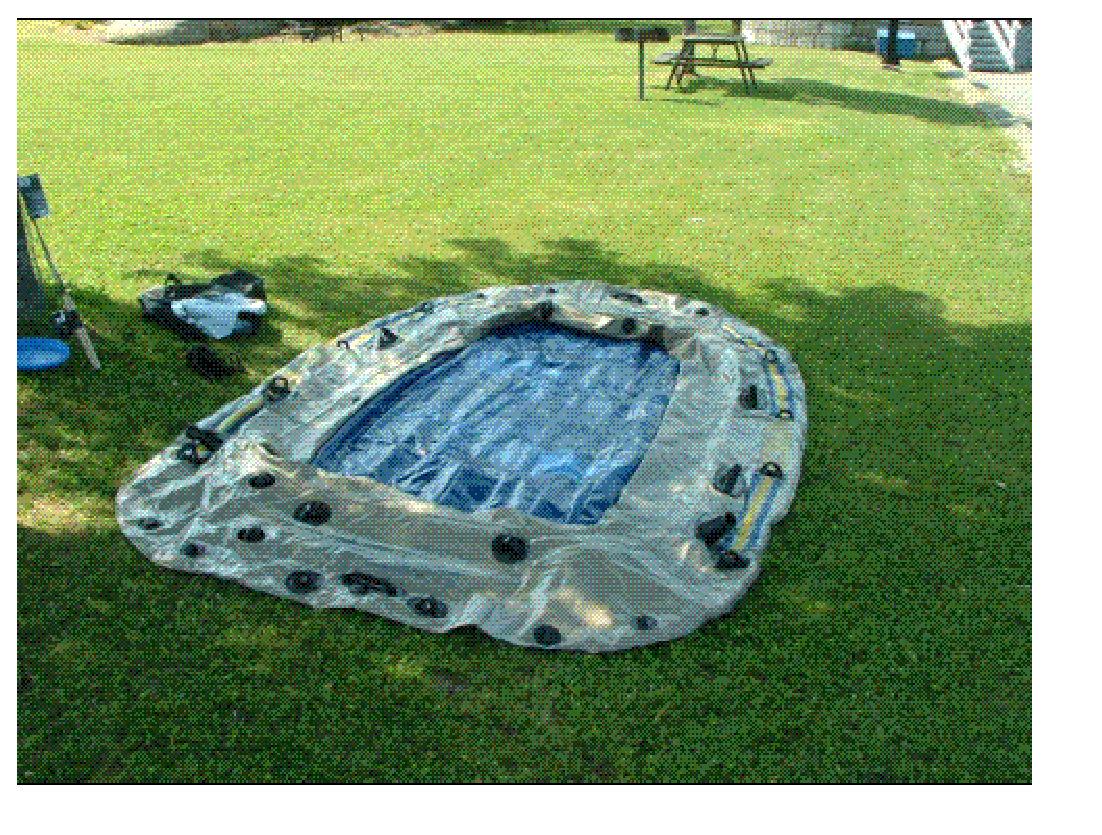
\epsfig{file=fig1.eps,width=3.5in}
Which one of the following is missing in it?
  
  
\noindent\hspace{3.0in} \begin{tabular}{|l|}
\hline
Your choice \\
\hline
 \\ 
 \\ 
\hline
\end{tabular}
  
  
 
 
\noindent{\textbf{\large{
A.}}}
A frisbee
 
 
\noindent{\textbf{\large{
B.}}}
An air-boat
 
 
\noindent{\textbf{\large{
C.}}}
A truck
 
 
\noindent{\textbf{\large{
D.}}}
An airplane
 
 
\noindent{\textbf{\large{
E.}}}
A table
 
 
\noindent{\textbf{\large{
F.}}}
  Not any of aboves.
 
 
 
\vspace{0.3in}
   
   
\vspace{0.3in}
{\textbf{\LARGE{You have done all the above? A very good beginning, please go ahead.}}}
More constants the
Mass of electron
$m_e$$ =
9.109390 \times 10^{-31} $
kg
,
Universal gas constant
$R$$ =
8.315 $
J/(mol$\cdot $K)
,
$e$$ =
1.60217733 \times 10^{-19} $
C
, and
$m_p$$ =
1.6726231 \times 10^{-27} $
kg
%
may be very helpful.
\vspace{0.3in}
   
   
  
\vspace{0.2in}
  
\noindent\begin{tabular}{|l|}
\hline
 YOUR MARKS  \\
\hline
 \\ 
 \\ 
\hline
\end{tabular}
\hspace{0.05in} \begin{tabular}{|l|}
\hline
 Full Marks  \\
\hline
 \\ 
3.13 \\
\hline
\end{tabular}
{\textbf{\Large{QUESTION
26.2 
}}}
  
  
 
 
An object is subjected to an external net force $\mathbf{f}=
(90.0 , 9.0 , -8000.0) N$.
Its mass is known as $m= % 
50.0000 kg$. Please choose the
correct accelaration from the following choices.
 
  
  
\noindent\hspace{3.0in} \begin{tabular}{|l|}
\hline
Your choice \\
\hline
 \\ 
 \\ 
\hline
\end{tabular}
  
  
 
 
\noindent{\textbf{\large{
A.}}}
The accelaration is $  %
(
1.80,
.81,
-160.00)
ms^{-2} $.
 
 
\noindent{\textbf{\large{
B.}}}
The accelaration is $  %
(
4.24,
.81,
-160.00)
ms^{-2} $.
 
 
\noindent{\textbf{\large{
C.}}}
The accelaration is $  %
(
1.80,
.18,
-160.00)
ms^{-2} $.
 
 
\noindent{\textbf{\large{
D.}}}
The accelaration is $  %
(
4.24,
.18,
447.95)
ms^{-2} $.
 
 
\noindent{\textbf{\large{
E.}}}
The accelaration is $  %
(
4.24,
.18,
-160.00)
ms^{-2} $.
 
 
\noindent{\textbf{\large{
F.}}}
The accelaration is $  %
(
1.80,
.18,
447.95)
ms^{-2} $.
 
 
\noindent{\textbf{\large{
G.}}}
The accelaration is $  %
(
1.80,
.81,
447.95)
ms^{-2} $.
 
 
\noindent{\textbf{\large{
H.}}}
The accelaration is $  %
(
4.24,
.81,
447.95)
ms^{-2} $.
 
 
 

 

 
\vspace{0.3in}
  
\vspace{0.2in}
  
\noindent\begin{tabular}{|l|}
\hline
 YOUR MARKS  \\
\hline
 \\ 
 \\ 
\hline
\end{tabular}
\hspace{0.05in} \begin{tabular}{|l|}
\hline
 Full Marks  \\
\hline
 \\ 
1.56 \\
\hline
\end{tabular}
{\textbf{\Large{QUESTION
26.3 
}}}
  
  
 
An object is subjected to an external net force $\mathbf{f}=(
80.000 ,
5.0000,
-9000.0  )N$. Its mass is known as
$m= % 
58.0000  kg$. Please choose the correct accelaration
from the following choices.
 
  
  
\noindent\hspace{3.0in} \begin{tabular}{|l|}
\hline
Your choice \\
\hline
 \\ 
 \\ 
\hline
\end{tabular}
  
  
 
 
\noindent{\textbf{\large{
A.}}}
The accelaration is
$(
1.3793ms^{-2},
1117.2km/h^2,
-155.17ms^{-2}
).
$
 
 
\noindent{\textbf{\large{
B.}}}
The accelaration is
$(
5.7113ms^{-2},
3858.5km/h^2,
-155.17ms^{-2}
).
$
 
 
\noindent{\textbf{\large{
C.}}}
The accelaration is
$(
1.3793ms^{-2},
3858.5km/h^2,
533.37ms^{-2}
).
$
 
 
\noindent{\textbf{\large{
D.}}}
The accelaration is
$(
5.7113ms^{-2},
1117.2km/h^2,
533.37ms^{-2}
).
$
 
 
\noindent{\textbf{\large{
E.}}}
The accelaration is
$(
1.3793ms^{-2},
3858.5km/h^2,
-155.17ms^{-2}
).
$
 
 
\noindent{\textbf{\large{
F.}}}
The accelaration is
$(
1.3793ms^{-2},
1117.2km/h^2,
533.37ms^{-2}
).
$
 
 
\noindent{\textbf{\large{
G.}}}
 None of these.
 
 
 
 

 
\vspace{0.3in}
  
\vspace{0.2in}
  
\noindent\begin{tabular}{|l|}
\hline
 YOUR MARKS  \\
\hline
 \\ 
 \\ 
\hline
\end{tabular}
\hspace{0.05in} \begin{tabular}{|l|}
\hline
 Full Marks  \\
\hline
 \\ 
1.56 \\
\hline
\end{tabular}
{\textbf{\Large{QUESTION
26.4 
}}}
  
  
Please choose the correct one from the following statements:
  
  
\noindent\hspace{3.0in} \begin{tabular}{|l|}
\hline
Your choice \\
\hline
 \\ 
 \\ 
\hline
\end{tabular}
  
  
 
 
\noindent{\textbf{\large{
A.}}}
Canada has  %
35 provinces and  %
34 territories.
 
 
\noindent{\textbf{\large{
B.}}}
Canada has  %
33 provinces and  %
38 territories.
 
 
\noindent{\textbf{\large{
C.}}}
Canada has  %
34 provinces and  %
39 territories.
 
 
\noindent{\textbf{\large{
D.}}}
Canada has  %
36 provinces and  %
35 territories.
 
 
\noindent{\textbf{\large{
E.}}}
Canada has  %
37 provinces and  %
37 territories.
 
 
\noindent{\textbf{\large{
F.}}}
 None of above.
 
 
  
\vspace{0.2in}
  
\noindent\begin{tabular}{|l|}
\hline
 YOUR MARKS  \\
\hline
 \\ 
 \\ 
\hline
\end{tabular}
\hspace{0.05in} \begin{tabular}{|l|}
\hline
 Full Marks  \\
\hline
 \\ 
1.56 \\
\hline
\end{tabular}
{\textbf{\Large{QUESTION
26.5 
}}}
  
  
If any one of the following statements is correct, please fill the box ahead of it with $T$ .
If wrong, fill with $F$.
 
\noindent\begin{tabular}{|l|l|}\hline Your&\hspace{.2in} \\ answer&\hspace{.2in} \\ \hline \end{tabular}
1. $ % 
78$ is an  % 
odd number.
 
\noindent\begin{tabular}{|l|l|}\hline Your&\hspace{.2in} \\ answer&\hspace{.2in} \\ \hline \end{tabular}
2.  % 
Toronto is in  % 
Ontario province.
 
\noindent\begin{tabular}{|l|l|}\hline Your&\hspace{.2in} \\ answer&\hspace{.2in} \\ \hline \end{tabular}
3.  % 
$\mathbf{F}=m\mathbf{a}$ is a mathmatical form of
Newton's Law of Universal Gravitation.
 

 
\vspace{0.3in}
  
\vspace{0.2in}
  
\noindent\begin{tabular}{|l|}
\hline
 YOUR MARKS  \\
\hline
 \\ 
 \\ 
\hline
\end{tabular}
\hspace{0.05in} \begin{tabular}{|l|}
\hline
 Full Marks  \\
\hline
 \\ 
3.13 \\
\hline
\end{tabular}
{\textbf{\Large{QUESTION
26.6 
}}}
  
  
Considering case-insensitivity, please match the following same strings.
  
  
\begin{tabular}{|l|l|l|}
 \hline
 Column Left & Column Right  & Your choinces \\ 
 \hline
{\textbf{\large{
A.}}}
er
  & 
ASDF(:)
 & 
 \\ 
 \hline
{\textbf{\large{
B.}}}
Er
  & 
b
 & 
 \\ 
 \hline
{\textbf{\large{
C.}}}
B
  & 
eR
 & 
 \\ 
 \hline
{\textbf{\large{
D.}}}
asdf(:)
  & 
a
 & 
 \\ 
 \hline
{\textbf{\large{
E.}}}
A
  & 
ER
 & 
 \\ 
 \hline
 \end{tabular}
  
  
 
   
   
\vspace{0.3in}
{\textbf{\LARGE{You have done all the above? Excellent! Not much left, please continue.}}}
\vspace{0.3in}
   
   
  
\vspace{0.2in}
  
\noindent\begin{tabular}{|l|}
\hline
 YOUR MARKS  \\
\hline
 \\ 
 \\ 
\hline
\end{tabular}
\hspace{0.05in} \begin{tabular}{|l|}
\hline
 Full Marks  \\
\hline
 \\ 
12.50 \\
\hline
\end{tabular}
{\textbf{\Large{QUESTION
26.7 
}}}
  
  
 
An object is subjected to an external net force $\mathbf{f}=
(90.0 , 7.0 , -7000.0) N$.
Its mass is known as $m= % 
58.0 kg$.
Please choose the correct accelaration from the following choices.
  
  
\noindent\hspace{3.0in} \begin{tabular}{|l|}
\hline
Your choice \\
\hline
 \\ 
 \\ 
\hline
\end{tabular}
  
  
 
 
\noindent{\textbf{\large{
A.}}}
  The accelaration is $  %
(
1.55,
.12,
-120.69)
ms^{-2} $.
 
 
\noindent{\textbf{\large{
B.}}}
  The accelaration is $  %
(
-3.12,
.39,
-120.69)
ms^{-2} $.
 
 
\noindent{\textbf{\large{
C.}}}
  The accelaration is $  %
(
1.55,
.39,
-120.69)
ms^{-2} $.
 
 
\noindent{\textbf{\large{
D.}}}
  The accelaration is $  %
(
-3.12,
.12,
-120.69)
ms^{-2} $.
 
 
 

 
 
\vspace{0.3in}
  
\vspace{0.2in}
  
\noindent\begin{tabular}{|l|}
\hline
 YOUR MARKS  \\
\hline
 \\ 
 \\ 
\hline
\end{tabular}
\hspace{0.05in} \begin{tabular}{|l|}
\hline
 Full Marks  \\
\hline
 \\ 
12.50 \\
\hline
\end{tabular}
{\textbf{\Large{QUESTION
26.8 
}}}
  
  
 
$ \left( \begin{array}{ccccccccc}
           4 & 
           7 & 
           5 & 
           6 \\ 
           6 & 
           6 & 
           7 & 
           5 \\ 
           4 & 
           4 & 
           4 & 
           4
\end{array}\right) \times
\left( \begin{array}{c}
           2 \\ 
           2 \\ 
           2 \\ 
           2
\end{array}\right) $ =?
 
 
$  % 
 \left( \begin{array}
 {
 c
 c
 }
 \varepsilon & 
 \rho \\ 
 \sigma & 
 \beta \\ 
 \Lambda & 
 \Delta \\ 
 \Omega & 
                    \Xi
 \end{array} \right)
 \left( \begin{array}
 {
 c
 }
 \gamma \\ 
 \gamma
 \end{array} \right)
$ =?
 

 

 
\vspace{0.3in}
  
\vspace{0.2in}
  
\noindent\begin{tabular}{|l|}
\hline
 YOUR MARKS  \\
\hline
 \\ 
 \\ 
\hline
\end{tabular}
\hspace{0.05in} \begin{tabular}{|l|}
\hline
 Full Marks  \\
\hline
 \\ 
1.56 \\
\hline
\end{tabular}
{\textbf{\Large{QUESTION
26.9 
}}}
  
  
 
 
% First root
% Second root

 
Please solve the following equation:
\begin{eqnarray*}
7 \times x^2  % 
-28
                 \times x    % 
-539 =0
\end{eqnarray*}
 

 

 
\vspace{0.3in}
   
   
 \vspace{0.2in}
Here are still some constants for use:
 
 
\noindent\begin{tabular}{|l|l|l|}
\hline
Constant & Symbol & Value \\
\hline
 
Mass of proton &
$m_p$ &
 $ 1.6726231 \times 10^{-27} $
kg \\
\hline
 
Boltzmann's constant &
$k$ &
 $ 1.381 \times 10^{-23} $
J/K \\
\hline
 
\end{tabular}
 
Thank you very much for answering these questions!
 
{\textbf{\large{Please be advised}}} that in this paper there are questions from
26.1 through
26.9.
And any one of them may contain more than one sub-question, thus the total number
of sub-questions here is around 14, of which
13 should be answered.
 
   
   
   
   
\vspace{1.0in} 
{\textbf{\large{ *** END OF PAPER, THANKS *** }}} 
   
   
\hspace{1.0in} By: 
         239(         26,          34)
   
   
   
   
\newpage 
\setcounter{page}{ 
    27001 } 
   
   
   
   
\noindent\begin{tabular}{|l|}
\hline
YOUR NAME (FIRST, ... LAST)  \\
\hline
 \\ 
 \\ 
\hline
\end{tabular}
\hspace{0.05in} \begin{tabular}{|l|}
\hline
 YOUR   ID   INFORMATION  \\
\hline
 \\ 
 \\ 
\hline
\end{tabular}
   
   
\vspace{0.2in}\noindent\begin{tabular}{|l|}
\hline
YOUR TOTAL MARKS  \\
\hline
 \\ 
 \\ 
\hline
\end{tabular}
\hspace{0.05in} \begin{tabular}{|l|}
\hline
TOTAL FULL MARKS  \\
\hline
 \\ 
100.00 \\
\hline
\end{tabular}
   
   
 \vspace{0.2in}
 
 
{\Huge  THIS IS AN EXAMPLE OF}
 
{\Huge  PERSONALIZED TESTS. }
 
If needed, please use the following constants.
 
 
 
\noindent\begin{tabular}{|l|l|l|}
\hline
Constant & Symbol & Value \\
\hline
Acceleration due to earth's gravity &
$g$ &
 $ 9.80 $
m/s$^2$ \\
\hline
Avogadro's number &
$N_A$ &
 $ 6.0221367 \times 10^{23} $
mol$^{-1}$ \\
\hline
Boltzmann's constant &
$k$ &
 $ 1.380658 \times 10^{-23} $
J/K \\
\hline
Coulomb's constant &
$k$ &
 $ 8.99 \times 10^{9} $
N$\cdot $m$^2$/C$^2$ \\
\hline
Electron charge magnitiude &
$e$ &
 $ 1.60217733 \times 10^{-19} $
C \\
\hline
Permeability of free space &
$\mu _0$ &
 $ 1.25663706 \times 10^{-6} $
T$\cdot $m/A \\
\hline
Permittivity of free space &
$\epsilon _0$ &
 $ 8.854187817 \times 10^{-12} $
C$^2$/(N$\cdot $m$^2$) \\
\hline
Pi &
$\pi$ &
 $ 3.14159265 $
$ $ \\
\hline
Planck's constant &
$h$ &
 $ 6.6260755 \times 10^{-34} $
J$\cdot $s \\
\hline
Mass of electron &
$m_e$ &
 $ 9.1093897 \times 10^{-31} $
kg \\
\hline
\end{tabular}
 
 
\noindent\begin{tabular}{|l|l|l|}
\hline
Constant & Symbol & Value \\
\hline
Mass of neutron &
$m_n$ &
 $ 1.6749286 \times 10^{-27} $
kg \\
\hline
Mass of proton &
$m_p$ &
 $ 1.6726231 \times 10^{-27} $
kg \\
\hline
Speed of light in vacuum &
$c$ &
 $ 299792458. $
m/s \\
\hline
Universal gravitational constant &
$G$ &
 $ 6.67259 \times 10^{-11} $
N$\cdot $m$^2$/kg$^2$ \\
\hline
Universal gas constant &
$R$ &
 $ 8.314510 $
J/(mol$\cdot $K) \\
\hline
\end{tabular}
 
 
{\textbf{\large{Please be advised}}} that in this paper there are questions from
27.1 through
27.9.
And any one of them may contain more than one sub-question, thus the total number
of sub-questions here is around 14, of which
13 should be answered.
 
\vspace{0.3in}
 
 
   
   
  
\vspace{0.2in}
  
\noindent\begin{tabular}{|l|}
\hline
 YOUR MARKS  \\
\hline
 \\ 
 \\ 
\hline
\end{tabular}
\hspace{0.05in} \begin{tabular}{|l|}
\hline
 Full Marks  \\
\hline
 \\ 
62.50 \\
\hline
\end{tabular}
{\textbf{\Large{QUESTION
27.1 
}}}
  
  
 
{\textbf{\Large{Please answer ONLY
5 of the following
6 questions (Questions
27.1.1 through
27.1.6). }}}
 
Here are still some constants for use in the following questions:
 
 
\noindent\begin{tabular}{|l|l|l|}
\hline
Constant & Symbol & Value \\
\hline
 
Boltzmann's constant &
$k$ &
 $ 1.381 \times 10^{-23} $
J/K \\
\hline
 
Avogadro's number &
$N_A$ &
 $ 6.022 \times 10^{23} $
mol$^{-1}$ \\
\hline
 
Mass of electron &
$m_e$ &
 $ 9.1093897 \times 10^{-31} $
kg \\
\hline
 
\end{tabular}
 
  
\vspace{0.2in}
  
         \begin{tabular}{|l|}
\hline
 Your marks  \\
\hline
 \\ 
 \\ 
\hline
\end{tabular}
\hspace{0.05in} \begin{tabular}{|l|}
\hline
 Full marks  \\
\hline
 \\ 
12.50 \\
\hline
\end{tabular}
{\textbf{\Large{Question
27.1.1 
}}}
  
  
 
An object is subjected to an external net force $\mathbf{f}=(
90.0 ,
6.0,
-3000.0  )N$. Its mass is known as
$m= % 
52.0  kg$. Please choose the correct accelaration
from the following choices.
 
  
  
\noindent\hspace{3.0in} \begin{tabular}{|l|}
\hline
Your choice \\
\hline
 \\ 
 \\ 
\hline
\end{tabular}
  
  
 
 
\noindent{\textbf{\large{
A.}}}
The accelaration is
$(
1.7308ms^{-2},
.54163ms^{-2},
-747692.km/h^2
).
$
 
 
\noindent{\textbf{\large{
B.}}}
The accelaration is
$(
4.9623ms^{-2},
.54163ms^{-2},
3.3972 \times 10^{6}km/h^2
).
$
 
 
\noindent{\textbf{\large{
C.}}}
The accelaration is
$(
1.7308ms^{-2},
.54163ms^{-2},
3.3972 \times 10^{6}km/h^2
).
$
 
 
\noindent{\textbf{\large{
D.}}}
The accelaration is
$(
4.9623ms^{-2},
.11538ms^{-2},
3.3972 \times 10^{6}km/h^2
).
$
 
 
\noindent{\textbf{\large{
E.}}}
none of these.
 
 
 
 

 
\vspace{0.3in}
  
\vspace{0.2in}
  
         \begin{tabular}{|l|}
\hline
 Your marks  \\
\hline
 \\ 
 \\ 
\hline
\end{tabular}
\hspace{0.05in} \begin{tabular}{|l|}
\hline
 Full marks  \\
\hline
 \\ 
12.50 \\
\hline
\end{tabular}
{\textbf{\Large{Question
27.1.2 
}}}
  
  
See the following picture.
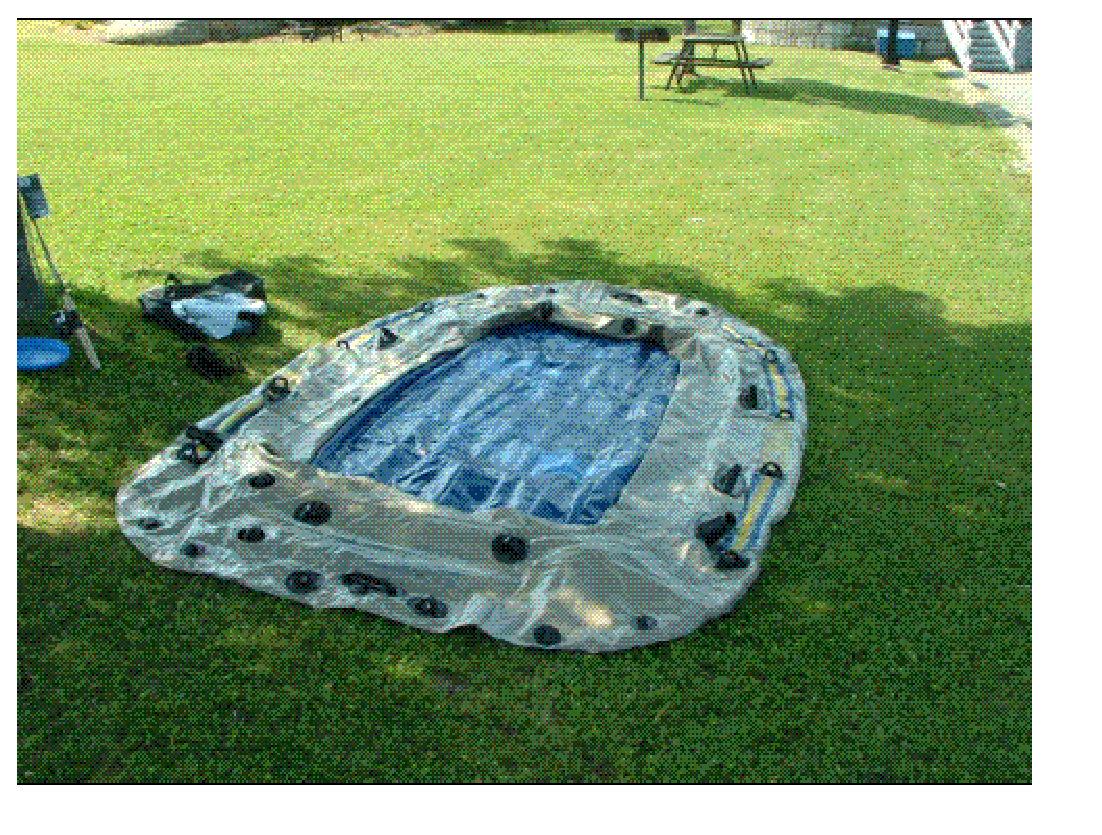
\epsfig{file=fig1.eps,width=3.5in}
Which one of the following is missing in it?
  
  
\noindent\hspace{3.0in} \begin{tabular}{|l|}
\hline
Your choice \\
\hline
 \\ 
 \\ 
\hline
\end{tabular}
  
  
 
 
\noindent{\textbf{\large{
A.}}}
An air-boat
 
 
\noindent{\textbf{\large{
B.}}}
Lawn
 
 
\noindent{\textbf{\large{
C.}}}
A truck
 
 
\noindent{\textbf{\large{
D.}}}
An airplane
 
 
\noindent{\textbf{\large{
E.}}}
A table
 
 
\noindent{\textbf{\large{
F.}}}
  Not any of aboves.
 
 
 
\vspace{0.3in}
  
\vspace{0.2in}
  
         \begin{tabular}{|l|}
\hline
 Your marks  \\
\hline
 \\ 
 \\ 
\hline
\end{tabular}
\hspace{0.05in} \begin{tabular}{|l|}
\hline
 Full marks  \\
\hline
 \\ 
12.50 \\
\hline
\end{tabular}
{\textbf{\Large{Question
27.1.3 
}}}
  
  
 
An object is subjected to an external net force $\mathbf{f}=(
50.0,  % 
5.0,
-5000.0  )N$. Its mass is known as
$m= % 
50.0 kg$. Please calculate its accelaration.
 
 

 

 
\vspace{0.3in}
  
\vspace{0.2in}
  
         \begin{tabular}{|l|}
\hline
 Your marks  \\
\hline
 \\ 
 \\ 
\hline
\end{tabular}
\hspace{0.05in} \begin{tabular}{|l|}
\hline
 Full marks  \\
\hline
 \\ 
12.50 \\
\hline
\end{tabular}
{\textbf{\Large{Question
27.1.4 
}}}
  
  
In a hotel, the possiblity of  % 
smoking customer is
$a =  % 
7.0 \times 10^{-2}$, and the possiblity of  % 
equal or above 30 years old customer is $ b =  % 
.8200$.
Please calculate the possiblity of  % 
 non-smoking and  % 
under 30 years old customer.
 

 

 
\vspace{0.3in}
  
\vspace{0.2in}
  
         \begin{tabular}{|l|}
\hline
 Your marks  \\
\hline
 \\ 
 \\ 
\hline
\end{tabular}
\hspace{0.05in} \begin{tabular}{|l|}
\hline
 Full marks  \\
\hline
 \\ 
12.50 \\
\hline
\end{tabular}
{\textbf{\Large{Question
27.1.5 
}}}
  
  
What is the operation between $a= % 
5$ and $b= % 
4$:
$a$  % 
$\times$ $b=?$ Please also calculate it.

 
\vspace{0.3in}
  
\vspace{0.2in}
  
         \begin{tabular}{|l|}
\hline
 Your marks  \\
\hline
 \\ 
 \\ 
\hline
\end{tabular}
\hspace{0.05in} \begin{tabular}{|l|}
\hline
 Full marks  \\
\hline
 \\ 
12.50 \\
\hline
\end{tabular}
{\textbf{\Large{Question
27.1.6 
}}}
  
  
 
An object is subjected to an external net force $\mathbf{f}=(
30.0 ,
3.0,
-3000.0  )N$. Its mass is known as
$m= % 
52.0  kg$. Please choose the correct accelaration
from the following choices.
 
  
  
\noindent\hspace{3.0in} \begin{tabular}{|l|}
\hline
Your choice \\
\hline
 \\ 
 \\ 
\hline
\end{tabular}
  
  
 
 
\noindent{\textbf{\large{
A.}}}
The accelaration (vector) is
$(
22208.,
747.69 ,
-2.6185 \times 10^{6}
)km/h^2.
$
 
 
\noindent{\textbf{\large{
B.}}}
The accelaration (vector) is
$(
-35808.,
747.69 ,
-1.7989 \times 10^{6}
)km/h^2.
$
 
 
\noindent{\textbf{\large{
C.}}}
The accelaration (vector) is
$(
-34372.,
747.69 ,
-2.6185 \times 10^{6}
)km/h^2.
$
 
 
\noindent{\textbf{\large{
D.}}}
The accelaration (vector) is
$(
-34372.,
747.69 ,
2.4415 \times 10^{6}
)km/h^2.
$
 
 
\noindent{\textbf{\large{
E.}}}
The accelaration (vector) is
$(
-34372.,
747.69 ,
-747692.
)km/h^2.
$
 
 
\noindent{\textbf{\large{
F.}}}
The accelaration (vector) is
$(
7476.9,
747.69 ,
-2.6185 \times 10^{6}
)km/h^2.
$
 
 
\noindent{\textbf{\large{
G.}}}
The accelaration (vector) is
$(
7476.9,
747.69 ,
2.4415 \times 10^{6}
)km/h^2.
$
 
 
\noindent{\textbf{\large{
H.}}}
The accelaration (vector) is
$(
-35808.,
747.69 ,
2.4415 \times 10^{6}
)km/h^2.
$
 
 
\noindent{\textbf{\large{
I.}}}
The accelaration (vector) is
$(
7476.9,
747.69 ,
-747692.
)km/h^2.
$
 
 
\noindent{\textbf{\large{
J.}}}
The accelaration (vector) is
$(
22208.,
747.69 ,
2.4415 \times 10^{6}
)km/h^2.
$
 
 
\noindent{\textbf{\large{
K.}}}
The accelaration (vector) is
$(
22208.,
747.69 ,
-1.7989 \times 10^{6}
)km/h^2.
$
 
 
\noindent{\textbf{\large{
L.}}}
The accelaration (vector) is
$(
-35808.,
747.69 ,
-747692.
)km/h^2.
$
 
 
 
 

 
 
\vspace{0.3in}
   
   
\vspace{0.3in}
{\textbf{\LARGE{You have done all the above? A very good beginning, please go ahead.}}}
More constants the
Mass of electron
$m_e$$ =
9.109390 \times 10^{-31} $
kg
,
Universal gas constant
$R$$ =
8.315 $
J/(mol$\cdot $K)
,
$e$$ =
1.60217733 \times 10^{-19} $
C
, and
$m_p$$ =
1.6726231 \times 10^{-27} $
kg
%
may be very helpful.
\vspace{0.3in}
   
   
  
\vspace{0.2in}
  
\noindent\begin{tabular}{|l|}
\hline
 YOUR MARKS  \\
\hline
 \\ 
 \\ 
\hline
\end{tabular}
\hspace{0.05in} \begin{tabular}{|l|}
\hline
 Full Marks  \\
\hline
 \\ 
3.13 \\
\hline
\end{tabular}
{\textbf{\Large{QUESTION
27.2 
}}}
  
  
Considering case-insensitivity, please match the following same strings.
  
  
\begin{tabular}{|l|l|l|}
 \hline
 Column Left & Column Right  & Your choinces \\ 
 \hline
{\textbf{\large{
A.}}}
er
  & 
b
 & 
 \\ 
 \hline
{\textbf{\large{
B.}}}
 A= %
6/ %
2

  & 
ER
 & 
 \\ 
 \hline
{\textbf{\large{
C.}}}
B
  & 
YJH
 & 
 \\ 
 \hline
{\textbf{\large{
D.}}}
asdf(:)
  & 
 a= %
3
 & 
 \\ 
 \hline
{\textbf{\large{
E.}}}
yjh
  & 
ASDF(:)
 & 
 \\ 
 \hline
 \end{tabular}
  
  
 
  
\vspace{0.2in}
  
\noindent\begin{tabular}{|l|}
\hline
 YOUR MARKS  \\
\hline
 \\ 
 \\ 
\hline
\end{tabular}
\hspace{0.05in} \begin{tabular}{|l|}
\hline
 Full Marks  \\
\hline
 \\ 
1.56 \\
\hline
\end{tabular}
{\textbf{\Large{QUESTION
27.3 
}}}
  
  
Please choose the correct one from the following statements:
  
  
\noindent\hspace{3.0in} \begin{tabular}{|l|}
\hline
Your choice \\
\hline
 \\ 
 \\ 
\hline
\end{tabular}
  
  
 
 
\noindent{\textbf{\large{
A.}}}
Canada has  %
10 provinces and  %
3 territories.
 
 
\noindent{\textbf{\large{
B.}}}
Canada has  %
37 provinces and  %
37 territories.
 
 
\noindent{\textbf{\large{
C.}}}
Canada has  %
36 provinces and  %
35 territories.
 
 
\noindent{\textbf{\large{
D.}}}
Canada has  %
35 provinces and  %
34 territories.
 
 
\noindent{\textbf{\large{
E.}}}
Canada has  %
33 provinces and  %
38 territories.
 
 
\noindent{\textbf{\large{
F.}}}
 None of above.
 
 
  
\vspace{0.2in}
  
\noindent\begin{tabular}{|l|}
\hline
 YOUR MARKS  \\
\hline
 \\ 
 \\ 
\hline
\end{tabular}
\hspace{0.05in} \begin{tabular}{|l|}
\hline
 Full Marks  \\
\hline
 \\ 
1.56 \\
\hline
\end{tabular}
{\textbf{\Large{QUESTION
27.4 
}}}
  
  
 
An object is subjected to an external net force $\mathbf{f}=(
80.000 ,
9.0000,
-9000.0  )N$. Its mass is known as
$m= % 
58.0000  kg$. Please choose the correct accelaration
from the following choices.
 
  
  
\noindent\hspace{3.0in} \begin{tabular}{|l|}
\hline
Your choice \\
\hline
 \\ 
 \\ 
\hline
\end{tabular}
  
  
 
 
\noindent{\textbf{\large{
A.}}}
The accelaration is
$(
-6.4083ms^{-2},
2011.0km/h^2,
-748.38ms^{-2}
).
$
 
 
\noindent{\textbf{\large{
B.}}}
The accelaration is
$(
-6.4083ms^{-2},
6610.6km/h^2,
-748.38ms^{-2}
).
$
 
 
\noindent{\textbf{\large{
C.}}}
The accelaration is
$(
1.3793ms^{-2},
2011.0km/h^2,
-748.38ms^{-2}
).
$
 
 
\noindent{\textbf{\large{
D.}}}
The accelaration is
$(
1.3793ms^{-2},
6610.6km/h^2,
-155.17ms^{-2}
).
$
 
 
\noindent{\textbf{\large{
E.}}}
The accelaration is
$(
1.3793ms^{-2},
2011.0km/h^2,
-155.17ms^{-2}
).
$
 
 
\noindent{\textbf{\large{
F.}}}
The accelaration is
$(
-6.4083ms^{-2},
6610.6km/h^2,
-155.17ms^{-2}
).
$
 
 
\noindent{\textbf{\large{
G.}}}
 None of these.
 
 
 
 

 
\vspace{0.3in}
  
\vspace{0.2in}
  
\noindent\begin{tabular}{|l|}
\hline
 YOUR MARKS  \\
\hline
 \\ 
 \\ 
\hline
\end{tabular}
\hspace{0.05in} \begin{tabular}{|l|}
\hline
 Full Marks  \\
\hline
 \\ 
3.13 \\
\hline
\end{tabular}
{\textbf{\Large{QUESTION
27.5 
}}}
  
  
 
 
An object is subjected to an external net force $\mathbf{f}=
(40.0 , 2.0 , -2000.0) N$.
Its mass is known as $m= % 
52.0000 kg$. Please choose the
correct accelaration from the following choices.
 
  
  
\noindent\hspace{3.0in} \begin{tabular}{|l|}
\hline
Your choice \\
\hline
 \\ 
 \\ 
\hline
\end{tabular}
  
  
 
 
\noindent{\textbf{\large{
A.}}}
The accelaration is $  %
(
3.47,
3.8 \times 10^{-2},
-38.462)
ms^{-2} $.
 
 
\noindent{\textbf{\large{
B.}}}
The accelaration is $  %
(
3.47,
3.8 \times 10^{-2},
-159.40)
ms^{-2} $.
 
 
\noindent{\textbf{\large{
C.}}}
The accelaration is $  %
(
.769,
.12,
-38.462)
ms^{-2} $.
 
 
\noindent{\textbf{\large{
D.}}}
The accelaration is $  %
(
.769,
3.8 \times 10^{-2},
-38.462)
ms^{-2} $.
 
 
\noindent{\textbf{\large{
E.}}}
The accelaration is $  %
(
.769,
3.8 \times 10^{-2},
-159.40)
ms^{-2} $.
 
 
\noindent{\textbf{\large{
F.}}}
The accelaration is $  %
(
3.47,
.12,
-159.40)
ms^{-2} $.
 
 
\noindent{\textbf{\large{
G.}}}
The accelaration is $  %
(
3.47,
.12,
-38.462)
ms^{-2} $.
 
 
\noindent{\textbf{\large{
H.}}}
The accelaration is $  %
(
.769,
.12,
-159.40)
ms^{-2} $.
 
 
 

 

 
\vspace{0.3in}
  
\vspace{0.2in}
  
\noindent\begin{tabular}{|l|}
\hline
 YOUR MARKS  \\
\hline
 \\ 
 \\ 
\hline
\end{tabular}
\hspace{0.05in} \begin{tabular}{|l|}
\hline
 Full Marks  \\
\hline
 \\ 
1.56 \\
\hline
\end{tabular}
{\textbf{\Large{QUESTION
27.6 
}}}
  
  
If any one of the following statements is correct, please fill the box ahead of it with $T$ .
If wrong, fill with $F$.
 
\noindent\begin{tabular}{|l|l|}\hline Your&\hspace{.2in} \\ answer&\hspace{.2in} \\ \hline \end{tabular}
1. $ % 
47$ is an  % 
even number.
 
\noindent\begin{tabular}{|l|l|}\hline Your&\hspace{.2in} \\ answer&\hspace{.2in} \\ \hline \end{tabular}
2.  % 
Montreal is in  % 
Ontario province.
 
\noindent\begin{tabular}{|l|l|}\hline Your&\hspace{.2in} \\ answer&\hspace{.2in} \\ \hline \end{tabular}
3.  % 
$\mathbf{F}=m\mathbf{a}$ is a mathmatical form of
the Newton's Second Law.
 

 
\vspace{0.3in}
   
   
\vspace{0.3in}
{\textbf{\LARGE{You have done all the above? Excellent! Not much left, please continue.}}}
\vspace{0.3in}
   
   
  
\vspace{0.2in}
  
\noindent\begin{tabular}{|l|}
\hline
 YOUR MARKS  \\
\hline
 \\ 
 \\ 
\hline
\end{tabular}
\hspace{0.05in} \begin{tabular}{|l|}
\hline
 Full Marks  \\
\hline
 \\ 
12.50 \\
\hline
\end{tabular}
{\textbf{\Large{QUESTION
27.7 
}}}
  
  
 
$ \left( \begin{array}{ccccccccc}
           5 & 
           7 & 
           7 & 
           6 \\ 
           5 & 
           4 & 
           6 & 
           5 \\ 
           6 & 
           6 & 
           5 & 
           5
\end{array}\right) \times
\left( \begin{array}{c}
           2 \\ 
           2 \\ 
           2 \\ 
           2
\end{array}\right) $ =?
 
 
$  % 
 \left( \begin{array}
 {
 c
 c
 }
                    \zeta & 
 \Theta \\ 
                    \Xi & 
 \Theta \\ 
 \eta & 
 \gamma \\ 
 \rho & 
 \delta
 \end{array} \right)
 \left( \begin{array}
 {
 c
 }
 \beta \\ 
 \beta
 \end{array} \right)
$ =?
 

 

 
\vspace{0.3in}
  
\vspace{0.2in}
  
\noindent\begin{tabular}{|l|}
\hline
 YOUR MARKS  \\
\hline
 \\ 
 \\ 
\hline
\end{tabular}
\hspace{0.05in} \begin{tabular}{|l|}
\hline
 Full Marks  \\
\hline
 \\ 
12.50 \\
\hline
\end{tabular}
{\textbf{\Large{QUESTION
27.8 
}}}
  
  
 
An object is subjected to an external net force $\mathbf{f}=
(80.0 , 8.0 , -8000.0) N$.
Its mass is known as $m= % 
58.0 kg$.
Please choose the correct accelaration from the following choices.
  
  
\noindent\hspace{3.0in} \begin{tabular}{|l|}
\hline
Your choice \\
\hline
 \\ 
 \\ 
\hline
\end{tabular}
  
  
 
 
\noindent{\textbf{\large{
A.}}}
  The accelaration is $  %
(
3.41,
.14,
533.78)
ms^{-2} $.
 
 
\noindent{\textbf{\large{
B.}}}
  The accelaration is $  %
(
1.38,
.14,
-137.93)
ms^{-2} $.
 
 
\noindent{\textbf{\large{
C.}}}
  The accelaration is $  %
(
1.38,
.14,
533.78)
ms^{-2} $.
 
 
\noindent{\textbf{\large{
D.}}}
  The accelaration is $  %
(
1.38,
.57,
533.78)
ms^{-2} $.
 
 
 

 
 
\vspace{0.3in}
  
\vspace{0.2in}
  
\noindent\begin{tabular}{|l|}
\hline
 YOUR MARKS  \\
\hline
 \\ 
 \\ 
\hline
\end{tabular}
\hspace{0.05in} \begin{tabular}{|l|}
\hline
 Full Marks  \\
\hline
 \\ 
1.56 \\
\hline
\end{tabular}
{\textbf{\Large{QUESTION
27.9 
}}}
  
  
 
 
% First root
% Second root

 
Please solve the following equation:
\begin{eqnarray*}
9 \times x^2  % 
-108
                 \times x    % 
-2925 =0
\end{eqnarray*}
 

 

 
\vspace{0.3in}
   
   
 \vspace{0.2in}
Here are still some constants for use:
 
 
\noindent\begin{tabular}{|l|l|l|}
\hline
Constant & Symbol & Value \\
\hline
 
Mass of proton &
$m_p$ &
 $ 1.6726231 \times 10^{-27} $
kg \\
\hline
 
Boltzmann's constant &
$k$ &
 $ 1.381 \times 10^{-23} $
J/K \\
\hline
 
\end{tabular}
 
Thank you very much for answering these questions!
 
{\textbf{\large{Please be advised}}} that in this paper there are questions from
27.1 through
27.9.
And any one of them may contain more than one sub-question, thus the total number
of sub-questions here is around 14, of which
13 should be answered.
 
   
   
   
   
\vspace{1.0in} 
{\textbf{\large{ *** END OF PAPER, THANKS *** }}} 
   
   
\hspace{1.0in} By: 
         239(         26,          34)
   
   
   
   
\newpage 
\setcounter{page}{ 
    28001 } 
   
   
   
   
\noindent\begin{tabular}{|l|}
\hline
YOUR NAME (FIRST, ... LAST)  \\
\hline
 \\ 
 \\ 
\hline
\end{tabular}
\hspace{0.05in} \begin{tabular}{|l|}
\hline
 YOUR   ID   INFORMATION  \\
\hline
 \\ 
 \\ 
\hline
\end{tabular}
   
   
\vspace{0.2in}\noindent\begin{tabular}{|l|}
\hline
YOUR TOTAL MARKS  \\
\hline
 \\ 
 \\ 
\hline
\end{tabular}
\hspace{0.05in} \begin{tabular}{|l|}
\hline
TOTAL FULL MARKS  \\
\hline
 \\ 
100.00 \\
\hline
\end{tabular}
   
   
 \vspace{0.2in}
 
 
{\Huge  THIS IS AN EXAMPLE OF}
 
{\Huge  PERSONALIZED TESTS. }
 
If needed, please use the following constants.
 
 
 
\noindent\begin{tabular}{|l|l|l|}
\hline
Constant & Symbol & Value \\
\hline
Acceleration due to earth's gravity &
$g$ &
 $ 9.80 $
m/s$^2$ \\
\hline
Avogadro's number &
$N_A$ &
 $ 6.0221367 \times 10^{23} $
mol$^{-1}$ \\
\hline
Boltzmann's constant &
$k$ &
 $ 1.380658 \times 10^{-23} $
J/K \\
\hline
Coulomb's constant &
$k$ &
 $ 8.99 \times 10^{9} $
N$\cdot $m$^2$/C$^2$ \\
\hline
Electron charge magnitiude &
$e$ &
 $ 1.60217733 \times 10^{-19} $
C \\
\hline
Permeability of free space &
$\mu _0$ &
 $ 1.25663706 \times 10^{-6} $
T$\cdot $m/A \\
\hline
Permittivity of free space &
$\epsilon _0$ &
 $ 8.854187817 \times 10^{-12} $
C$^2$/(N$\cdot $m$^2$) \\
\hline
Pi &
$\pi$ &
 $ 3.14159265 $
$ $ \\
\hline
Planck's constant &
$h$ &
 $ 6.6260755 \times 10^{-34} $
J$\cdot $s \\
\hline
Mass of electron &
$m_e$ &
 $ 9.1093897 \times 10^{-31} $
kg \\
\hline
\end{tabular}
 
 
\noindent\begin{tabular}{|l|l|l|}
\hline
Constant & Symbol & Value \\
\hline
Mass of neutron &
$m_n$ &
 $ 1.6749286 \times 10^{-27} $
kg \\
\hline
Mass of proton &
$m_p$ &
 $ 1.6726231 \times 10^{-27} $
kg \\
\hline
Speed of light in vacuum &
$c$ &
 $ 299792458. $
m/s \\
\hline
Universal gravitational constant &
$G$ &
 $ 6.67259 \times 10^{-11} $
N$\cdot $m$^2$/kg$^2$ \\
\hline
Universal gas constant &
$R$ &
 $ 8.314510 $
J/(mol$\cdot $K) \\
\hline
\end{tabular}
 
 
{\textbf{\large{Please be advised}}} that in this paper there are questions from
28.1 through
28.9.
And any one of them may contain more than one sub-question, thus the total number
of sub-questions here is around 14, of which
13 should be answered.
 
\vspace{0.3in}
 
 
   
   
  
\vspace{0.2in}
  
\noindent\begin{tabular}{|l|}
\hline
 YOUR MARKS  \\
\hline
 \\ 
 \\ 
\hline
\end{tabular}
\hspace{0.05in} \begin{tabular}{|l|}
\hline
 Full Marks  \\
\hline
 \\ 
62.50 \\
\hline
\end{tabular}
{\textbf{\Large{QUESTION
28.1 
}}}
  
  
 
{\textbf{\Large{Please answer ONLY
5 of the following
6 questions (Questions
28.1.1 through
28.1.6). }}}
 
Here are still some constants for use in the following questions:
 
 
\noindent\begin{tabular}{|l|l|l|}
\hline
Constant & Symbol & Value \\
\hline
 
Boltzmann's constant &
$k$ &
 $ 1.381 \times 10^{-23} $
J/K \\
\hline
 
Avogadro's number &
$N_A$ &
 $ 6.022 \times 10^{23} $
mol$^{-1}$ \\
\hline
 
Mass of electron &
$m_e$ &
 $ 9.1093897 \times 10^{-31} $
kg \\
\hline
 
\end{tabular}
 
  
\vspace{0.2in}
  
         \begin{tabular}{|l|}
\hline
 Your marks  \\
\hline
 \\ 
 \\ 
\hline
\end{tabular}
\hspace{0.05in} \begin{tabular}{|l|}
\hline
 Full marks  \\
\hline
 \\ 
12.50 \\
\hline
\end{tabular}
{\textbf{\Large{Question
28.1.1 
}}}
  
  
In a hotel, the possiblity of  % 
smoking customer is
$a =  % 
.580$, and the possiblity of  % 
 under 30 years old customer is $ b =  % 
.6200$.
Please calculate the possiblity of  % 
 non-smoking and  % 
equal or above 30 years old customer.
 

 

 
\vspace{0.3in}
  
\vspace{0.2in}
  
         \begin{tabular}{|l|}
\hline
 Your marks  \\
\hline
 \\ 
 \\ 
\hline
\end{tabular}
\hspace{0.05in} \begin{tabular}{|l|}
\hline
 Full marks  \\
\hline
 \\ 
12.50 \\
\hline
\end{tabular}
{\textbf{\Large{Question
28.1.2 
}}}
  
  
 
An object is subjected to an external net force $\mathbf{f}=(
80.0 ,
4.0,
-6000.0  )N$. Its mass is known as
$m= % 
58.0  kg$. Please choose the correct accelaration
from the following choices.
 
  
  
\noindent\hspace{3.0in} \begin{tabular}{|l|}
\hline
Your choice \\
\hline
 \\ 
 \\ 
\hline
\end{tabular}
  
  
 
 
\noindent{\textbf{\large{
A.}}}
The accelaration (vector) is
$(
-79300.,
893.79 ,
6.1195 \times 10^{6}
)km/h^2.
$
 
 
\noindent{\textbf{\large{
B.}}}
The accelaration (vector) is
$(
17876.,
893.79 ,
-6.0272 \times 10^{6}
)km/h^2.
$
 
 
\noindent{\textbf{\large{
C.}}}
The accelaration (vector) is
$(
17876.,
893.79 ,
-1.3407 \times 10^{6}
)km/h^2.
$
 
 
\noindent{\textbf{\large{
D.}}}
The accelaration (vector) is
$(
-59537.,
893.79 ,
5.9065 \times 10^{6}
)km/h^2.
$
 
 
\noindent{\textbf{\large{
E.}}}
The accelaration (vector) is
$(
-59537.,
893.79 ,
-1.3407 \times 10^{6}
)km/h^2.
$
 
 
\noindent{\textbf{\large{
F.}}}
The accelaration (vector) is
$(
-59537.,
893.79 ,
-6.0272 \times 10^{6}
)km/h^2.
$
 
 
\noindent{\textbf{\large{
G.}}}
The accelaration (vector) is
$(
36162.,
893.79 ,
5.9065 \times 10^{6}
)km/h^2.
$
 
 
\noindent{\textbf{\large{
H.}}}
The accelaration (vector) is
$(
17876.,
893.79 ,
6.1195 \times 10^{6}
)km/h^2.
$
 
 
\noindent{\textbf{\large{
I.}}}
The accelaration (vector) is
$(
-79300.,
893.79 ,
-6.0272 \times 10^{6}
)km/h^2.
$
 
 
\noindent{\textbf{\large{
J.}}}
The accelaration (vector) is
$(
36162.,
893.79 ,
-1.3407 \times 10^{6}
)km/h^2.
$
 
 
\noindent{\textbf{\large{
K.}}}
The accelaration (vector) is
$(
36162.,
893.79 ,
6.1195 \times 10^{6}
)km/h^2.
$
 
 
\noindent{\textbf{\large{
L.}}}
The accelaration (vector) is
$(
-79300.,
893.79 ,
5.9065 \times 10^{6}
)km/h^2.
$
 
 
 
 

 
 
\vspace{0.3in}
  
\vspace{0.2in}
  
         \begin{tabular}{|l|}
\hline
 Your marks  \\
\hline
 \\ 
 \\ 
\hline
\end{tabular}
\hspace{0.05in} \begin{tabular}{|l|}
\hline
 Full marks  \\
\hline
 \\ 
12.50 \\
\hline
\end{tabular}
{\textbf{\Large{Question
28.1.3 
}}}
  
  
See the following picture.
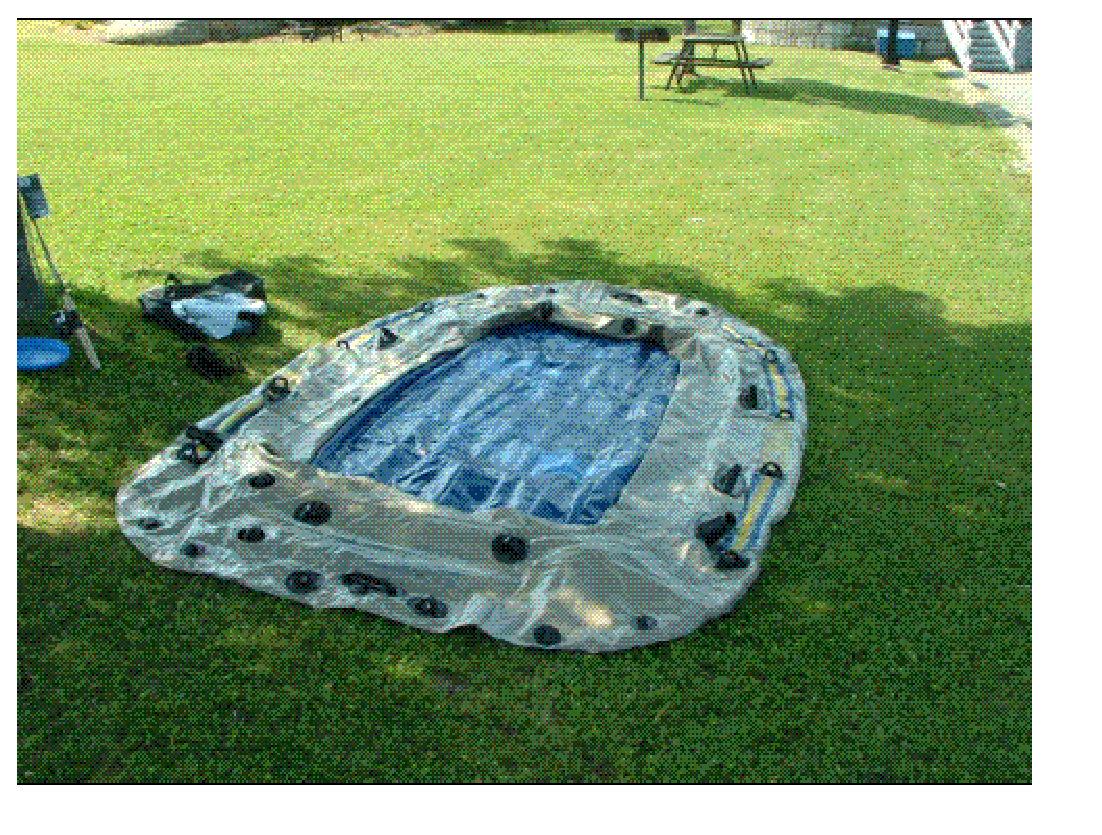
\epsfig{file=fig1.eps,width=3.5in}
Which one of the following is missing in it?
  
  
\noindent\hspace{3.0in} \begin{tabular}{|l|}
\hline
Your choice \\
\hline
 \\ 
 \\ 
\hline
\end{tabular}
  
  
 
 
\noindent{\textbf{\large{
A.}}}
An air-boat
 
 
\noindent{\textbf{\large{
B.}}}
Lawn
 
 
\noindent{\textbf{\large{
C.}}}
An airplane
 
 
\noindent{\textbf{\large{
D.}}}
A truck
 
 
\noindent{\textbf{\large{
E.}}}
A table
 
 
\noindent{\textbf{\large{
F.}}}
  Not any of aboves.
 
 
 
\vspace{0.3in}
  
\vspace{0.2in}
  
         \begin{tabular}{|l|}
\hline
 Your marks  \\
\hline
 \\ 
 \\ 
\hline
\end{tabular}
\hspace{0.05in} \begin{tabular}{|l|}
\hline
 Full marks  \\
\hline
 \\ 
12.50 \\
\hline
\end{tabular}
{\textbf{\Large{Question
28.1.4 
}}}
  
  
 
An object is subjected to an external net force $\mathbf{f}=(
70.0,  % 
4.0,
-9000.0  )N$. Its mass is known as
$m= % 
56.0 kg$. Please calculate its accelaration.
 
 

 

 
\vspace{0.3in}
  
\vspace{0.2in}
  
         \begin{tabular}{|l|}
\hline
 Your marks  \\
\hline
 \\ 
 \\ 
\hline
\end{tabular}
\hspace{0.05in} \begin{tabular}{|l|}
\hline
 Full marks  \\
\hline
 \\ 
12.50 \\
\hline
\end{tabular}
{\textbf{\Large{Question
28.1.5 
}}}
  
  
In a hotel, the possiblity of  % 
smoking customer is
$a =  % 
.120$, and the possiblity of  % 
equal-or-above 30 years old customer is $ b =  % 
.7000$.
Please fill the following form.
 
\noindent
\begin{tabular}{|l|l|}
\hline
Customer & Possibility \\
\hline
smoking  and   % 
equal-or-above 30 years old  & \\
\hline
smoking  and   % 
under 30 years old & \\
\hline
 non-smoking and   % 
equal-or-above 30 years old  & \\
\hline
 non-smoking and  % 
under 30 years old & \\
\hline
\end{tabular}
 
 
 

 

 
\vspace{0.3in}
  
\vspace{0.2in}
  
         \begin{tabular}{|l|}
\hline
 Your marks  \\
\hline
 \\ 
 \\ 
\hline
\end{tabular}
\hspace{0.05in} \begin{tabular}{|l|}
\hline
 Full marks  \\
\hline
 \\ 
12.50 \\
\hline
\end{tabular}
{\textbf{\Large{Question
28.1.6 
}}}
  
  
Let us use Newton's Law of Universal Gravitation to calculate the force
of the Sun acting on the eight planets. Let us suppose the mass of the
Sun is $ % 
9.00 \times 10^{24} kg$. With the mass and the
distance to the Sun of each planet in the following table, please fill
the blanks for the forces.
 
\vspace{0.2in}
 
 
\begin{tabular}{|l|l|l|l|}
\hline
The Planet & Mass ($kg$) & Distanace from Sun ($m$) & The Force ($N$)\\
\hline
Mercury  &
           $ % 
5.00000000 \times 10^{24} $   &
             $ % 
2.000000000 \times 10^{24} $    &
\\  \hline
Venus    &
           $ % 
6.00 \times 10^{24} $    &
             $ % 
4.00 \times 10^{24} $    &
\\  \hline
Earth    &
           $ % 
7.00 \times 10^{24} $    &
             $ % 
5.00 \times 10^{24} $    &
\\   \hline
Mars     &
           $ % 
7.00 \times 10^{24} $    &
             $ % 
7.00 \times 10^{24} $    &
\\   \hline
Jupiter  &
           $ % 
5.00 \times 10^{24} $    &
             $ % 
3.00 \times 10^{24} $    &
\\  \hline
Saturn   &
           $ % 
7.00 \times 10^{24}$    &
             $ % 
6.00 \times 10^{24}$    &
\\  \hline
Uranus   &
           $ % 
9.00 \times 10^{24} $    &
             $ % 
6.00 \times 10^{24} $    &
\\  \hline
Neptune  &
           $ % 
5.00 \times 10^{24} $    &
             $ % 
7.00 \times 10^{24} $    &
\\  \hline
 
\end{tabular}
 
 

 
 

 
\vspace{0.3in}
   
   
\vspace{0.3in}
{\textbf{\LARGE{You have done all the above? A very good beginning, please go ahead.}}}
More constants the
Mass of electron
$m_e$$ =
9.109390 \times 10^{-31} $
kg
,
Universal gas constant
$R$$ =
8.315 $
J/(mol$\cdot $K)
,
$e$$ =
1.60217733 \times 10^{-19} $
C
, and
$m_p$$ =
1.6726231 \times 10^{-27} $
kg
%
may be very helpful.
\vspace{0.3in}
   
   
  
\vspace{0.2in}
  
\noindent\begin{tabular}{|l|}
\hline
 YOUR MARKS  \\
\hline
 \\ 
 \\ 
\hline
\end{tabular}
\hspace{0.05in} \begin{tabular}{|l|}
\hline
 Full Marks  \\
\hline
 \\ 
1.56 \\
\hline
\end{tabular}
{\textbf{\Large{QUESTION
28.2 
}}}
  
  
If any one of the following statements is correct, please fill the box ahead of it with $T$ .
If wrong, fill with $F$.
 
\noindent\begin{tabular}{|l|l|}\hline Your&\hspace{.2in} \\ answer&\hspace{.2in} \\ \hline \end{tabular}
1. $ % 
80$ is an  % 
even number.
 
\noindent\begin{tabular}{|l|l|}\hline Your&\hspace{.2in} \\ answer&\hspace{.2in} \\ \hline \end{tabular}
2.  % 
Toronto is in  % 
Ontario province.
 
\noindent\begin{tabular}{|l|l|}\hline Your&\hspace{.2in} \\ answer&\hspace{.2in} \\ \hline \end{tabular}
3.  % 
$\left| \mathbf{F}\right| =Gm_1m_2r^{-2}$ is a mathmatical form of
the Newton's Second Law.
 

 
\vspace{0.3in}
  
\vspace{0.2in}
  
\noindent\begin{tabular}{|l|}
\hline
 YOUR MARKS  \\
\hline
 \\ 
 \\ 
\hline
\end{tabular}
\hspace{0.05in} \begin{tabular}{|l|}
\hline
 Full Marks  \\
\hline
 \\ 
1.56 \\
\hline
\end{tabular}
{\textbf{\Large{QUESTION
28.3 
}}}
  
  
Please choose the correct one from the following statements:
  
  
\noindent\hspace{3.0in} \begin{tabular}{|l|}
\hline
Your choice \\
\hline
 \\ 
 \\ 
\hline
\end{tabular}
  
  
 
 
\noindent{\textbf{\large{
A.}}}
Canada has  %
10 provinces and  %
3 territories.
 
 
\noindent{\textbf{\large{
B.}}}
Canada has  %
33 provinces and  %
38 territories.
 
 
\noindent{\textbf{\large{
C.}}}
Canada has  %
34 provinces and  %
39 territories.
 
 
\noindent{\textbf{\large{
D.}}}
Canada has  %
37 provinces and  %
37 territories.
 
 
\noindent{\textbf{\large{
E.}}}
Canada has  %
35 provinces and  %
34 territories.
 
 
\noindent{\textbf{\large{
F.}}}
 None of above.
 
 
  
\vspace{0.2in}
  
\noindent\begin{tabular}{|l|}
\hline
 YOUR MARKS  \\
\hline
 \\ 
 \\ 
\hline
\end{tabular}
\hspace{0.05in} \begin{tabular}{|l|}
\hline
 Full Marks  \\
\hline
 \\ 
3.13 \\
\hline
\end{tabular}
{\textbf{\Large{QUESTION
28.4 
}}}
  
  
Considering case-insensitivity, please match the following same strings.
  
  
\begin{tabular}{|l|l|l|}
 \hline
 Column Left & Column Right  & Your choinces \\ 
 \hline
{\textbf{\large{
A.}}}
asdf(:)
  & 
b
 & 
 \\ 
 \hline
{\textbf{\large{
B.}}}
B
  & 
a
 & 
 \\ 
 \hline
{\textbf{\large{
C.}}}
yjh
  & 
YJH
 & 
 \\ 
 \hline
{\textbf{\large{
D.}}}
A
  & 
eR
 & 
 \\ 
 \hline
{\textbf{\large{
E.}}}
er
  & 
ASDF(:)
 & 
 \\ 
 \hline
 \end{tabular}
  
  
 
  
\vspace{0.2in}
  
\noindent\begin{tabular}{|l|}
\hline
 YOUR MARKS  \\
\hline
 \\ 
 \\ 
\hline
\end{tabular}
\hspace{0.05in} \begin{tabular}{|l|}
\hline
 Full Marks  \\
\hline
 \\ 
3.13 \\
\hline
\end{tabular}
{\textbf{\Large{QUESTION
28.5 
}}}
  
  
 
 
An object is subjected to an external net force $\mathbf{f}=
(90.0 , 4.0 , -3000.0) N$.
Its mass is known as $m= % 
50.0000 kg$. Please choose the
correct accelaration from the following choices.
 
  
  
\noindent\hspace{3.0in} \begin{tabular}{|l|}
\hline
Your choice \\
\hline
 \\ 
 \\ 
\hline
\end{tabular}
  
  
 
 
\noindent{\textbf{\large{
A.}}}
The accelaration is $  %
(
1.80,
.31,
-60.000)
ms^{-2} $.
 
 
\noindent{\textbf{\large{
B.}}}
The accelaration is $  %
(
3.94,
.31,
202.99)
ms^{-2} $.
 
 
\noindent{\textbf{\large{
C.}}}
The accelaration is $  %
(
1.80,
8.0 \times 10^{-2},
202.99)
ms^{-2} $.
 
 
\noindent{\textbf{\large{
D.}}}
The accelaration is $  %
(
3.94,
8.0 \times 10^{-2},
-60.000)
ms^{-2} $.
 
 
\noindent{\textbf{\large{
E.}}}
The accelaration is $  %
(
3.94,
8.0 \times 10^{-2},
202.99)
ms^{-2} $.
 
 
\noindent{\textbf{\large{
F.}}}
The accelaration is $  %
(
1.80,
.31,
202.99)
ms^{-2} $.
 
 
\noindent{\textbf{\large{
G.}}}
The accelaration is $  %
(
1.80,
8.0 \times 10^{-2},
-60.000)
ms^{-2} $.
 
 
\noindent{\textbf{\large{
H.}}}
The accelaration is $  %
(
3.94,
.31,
-60.000)
ms^{-2} $.
 
 
 

 

 
\vspace{0.3in}
  
\vspace{0.2in}
  
\noindent\begin{tabular}{|l|}
\hline
 YOUR MARKS  \\
\hline
 \\ 
 \\ 
\hline
\end{tabular}
\hspace{0.05in} \begin{tabular}{|l|}
\hline
 Full Marks  \\
\hline
 \\ 
1.56 \\
\hline
\end{tabular}
{\textbf{\Large{QUESTION
28.6 
}}}
  
  
 
An object is subjected to an external net force $\mathbf{f}=(
90.000 ,
7.0000,
-8000.0  )N$. Its mass is known as
$m= % 
54.0000  kg$. Please choose the correct accelaration
from the following choices.
 
  
  
\noindent\hspace{3.0in} \begin{tabular}{|l|}
\hline
Your choice \\
\hline
 \\ 
 \\ 
\hline
\end{tabular}
  
  
 
 
\noindent{\textbf{\large{
A.}}}
The accelaration is
$(
1.6667ms^{-2},
-4788.6km/h^2,
-424.68ms^{-2}
).
$
 
 
\noindent{\textbf{\large{
B.}}}
The accelaration is
$(
1.6667ms^{-2},
1680.0km/h^2,
-424.68ms^{-2}
).
$
 
 
\noindent{\textbf{\large{
C.}}}
The accelaration is
$(
-4.8184ms^{-2},
-4788.6km/h^2,
-424.68ms^{-2}
).
$
 
 
\noindent{\textbf{\large{
D.}}}
The accelaration is
$(
-4.8184ms^{-2},
1680.0km/h^2,
-148.15ms^{-2}
).
$
 
 
\noindent{\textbf{\large{
E.}}}
The accelaration is
$(
1.6667ms^{-2},
1680.0km/h^2,
-148.15ms^{-2}
).
$
 
 
\noindent{\textbf{\large{
F.}}}
The accelaration is
$(
-4.8184ms^{-2},
-4788.6km/h^2,
-148.15ms^{-2}
).
$
 
 
\noindent{\textbf{\large{
G.}}}
 None of these.
 
 
 
 

 
\vspace{0.3in}
   
   
\vspace{0.3in}
{\textbf{\LARGE{You have done all the above? Excellent! Not much left, please continue.}}}
\vspace{0.3in}
   
   
  
\vspace{0.2in}
  
\noindent\begin{tabular}{|l|}
\hline
 YOUR MARKS  \\
\hline
 \\ 
 \\ 
\hline
\end{tabular}
\hspace{0.05in} \begin{tabular}{|l|}
\hline
 Full Marks  \\
\hline
 \\ 
12.50 \\
\hline
\end{tabular}
{\textbf{\Large{QUESTION
28.7 
}}}
  
  
 
$ \left( \begin{array}{ccccccccc}
           6 & 
           5 & 
           6 & 
           4 \\ 
           4 & 
           5 & 
           4 & 
           6 \\ 
           5 & 
           6 & 
           5 & 
           4
\end{array}\right) \times
\left( \begin{array}{c}
           2 \\ 
           2 \\ 
           2 \\ 
           2
\end{array}\right) $ =?
 
 
$  % 
 \left( \begin{array}
 {
 c
 c
 }
 \beta & 
 \Gamma \\ 
 \epsilon & 
 \beta \\ 
 \eta & 
 \beta \\ 
                    \Xi & 
 \epsilon
 \end{array} \right)
 \left( \begin{array}
 {
 c
 }
 \beta \\ 
 \gamma
 \end{array} \right)
$ =?
 

 

 
\vspace{0.3in}
  
\vspace{0.2in}
  
\noindent\begin{tabular}{|l|}
\hline
 YOUR MARKS  \\
\hline
 \\ 
 \\ 
\hline
\end{tabular}
\hspace{0.05in} \begin{tabular}{|l|}
\hline
 Full Marks  \\
\hline
 \\ 
12.50 \\
\hline
\end{tabular}
{\textbf{\Large{QUESTION
28.8 
}}}
  
  
 
An object is subjected to an external net force $\mathbf{f}=
(80.0 , 5.0 , -9000.0) N$.
Its mass is known as $m= % 
50.0 kg$.
Please choose the correct accelaration from the following choices.
  
  
\noindent\hspace{3.0in} \begin{tabular}{|l|}
\hline
Your choice \\
\hline
 \\ 
 \\ 
\hline
\end{tabular}
  
  
 
 
\noindent{\textbf{\large{
A.}}}
  The accelaration is $  %
(
7.22,
.10,
-180.00)
ms^{-2} $.
 
 
\noindent{\textbf{\large{
B.}}}
  The accelaration is $  %
(
1.60,
.10,
-180.00)
ms^{-2} $.
 
 
\noindent{\textbf{\large{
C.}}}
  The accelaration is $  %
(
7.22,
.47,
-180.00)
ms^{-2} $.
 
 
\noindent{\textbf{\large{
D.}}}
  The accelaration is $  %
(
7.22,
.47,
-620.64)
ms^{-2} $.
 
 
 

 
 
\vspace{0.3in}
  
\vspace{0.2in}
  
\noindent\begin{tabular}{|l|}
\hline
 YOUR MARKS  \\
\hline
 \\ 
 \\ 
\hline
\end{tabular}
\hspace{0.05in} \begin{tabular}{|l|}
\hline
 Full Marks  \\
\hline
 \\ 
1.56 \\
\hline
\end{tabular}
{\textbf{\Large{QUESTION
28.9 
}}}
  
  
 
 
% First root
% Second root

 
Please solve the following equation:
\begin{eqnarray*}
15 \times x^2  % 
+  % 
210
                 \times x    % 
-7905 =0
\end{eqnarray*}
 

 

 
\vspace{0.3in}
   
   
 \vspace{0.2in}
Here are still some constants for use:
 
 
\noindent\begin{tabular}{|l|l|l|}
\hline
Constant & Symbol & Value \\
\hline
 
Mass of proton &
$m_p$ &
 $ 1.6726231 \times 10^{-27} $
kg \\
\hline
 
Boltzmann's constant &
$k$ &
 $ 1.381 \times 10^{-23} $
J/K \\
\hline
 
\end{tabular}
 
Thank you very much for answering these questions!
 
{\textbf{\large{Please be advised}}} that in this paper there are questions from
28.1 through
28.9.
And any one of them may contain more than one sub-question, thus the total number
of sub-questions here is around 14, of which
13 should be answered.
 
   
   
   
   
\vspace{1.0in} 
{\textbf{\large{ *** END OF PAPER, THANKS *** }}} 
   
   
\hspace{1.0in} By: 
         239(         26,          34)
   
   
   
   
\newpage 
\setcounter{page}{ 
    29001 } 
   
   
   
   
\noindent\begin{tabular}{|l|}
\hline
YOUR NAME (FIRST, ... LAST)  \\
\hline
 \\ 
 \\ 
\hline
\end{tabular}
\hspace{0.05in} \begin{tabular}{|l|}
\hline
 YOUR   ID   INFORMATION  \\
\hline
 \\ 
 \\ 
\hline
\end{tabular}
   
   
\vspace{0.2in}\noindent\begin{tabular}{|l|}
\hline
YOUR TOTAL MARKS  \\
\hline
 \\ 
 \\ 
\hline
\end{tabular}
\hspace{0.05in} \begin{tabular}{|l|}
\hline
TOTAL FULL MARKS  \\
\hline
 \\ 
100.00 \\
\hline
\end{tabular}
   
   
 \vspace{0.2in}
 
 
{\Huge  THIS IS AN EXAMPLE OF}
 
{\Huge  PERSONALIZED TESTS. }
 
If needed, please use the following constants.
 
 
 
\noindent\begin{tabular}{|l|l|l|}
\hline
Constant & Symbol & Value \\
\hline
Acceleration due to earth's gravity &
$g$ &
 $ 9.80 $
m/s$^2$ \\
\hline
Avogadro's number &
$N_A$ &
 $ 6.0221367 \times 10^{23} $
mol$^{-1}$ \\
\hline
Boltzmann's constant &
$k$ &
 $ 1.380658 \times 10^{-23} $
J/K \\
\hline
Coulomb's constant &
$k$ &
 $ 8.99 \times 10^{9} $
N$\cdot $m$^2$/C$^2$ \\
\hline
Electron charge magnitiude &
$e$ &
 $ 1.60217733 \times 10^{-19} $
C \\
\hline
Permeability of free space &
$\mu _0$ &
 $ 1.25663706 \times 10^{-6} $
T$\cdot $m/A \\
\hline
Permittivity of free space &
$\epsilon _0$ &
 $ 8.854187817 \times 10^{-12} $
C$^2$/(N$\cdot $m$^2$) \\
\hline
Pi &
$\pi$ &
 $ 3.14159265 $
$ $ \\
\hline
Planck's constant &
$h$ &
 $ 6.6260755 \times 10^{-34} $
J$\cdot $s \\
\hline
Mass of electron &
$m_e$ &
 $ 9.1093897 \times 10^{-31} $
kg \\
\hline
\end{tabular}
 
 
\noindent\begin{tabular}{|l|l|l|}
\hline
Constant & Symbol & Value \\
\hline
Mass of neutron &
$m_n$ &
 $ 1.6749286 \times 10^{-27} $
kg \\
\hline
Mass of proton &
$m_p$ &
 $ 1.6726231 \times 10^{-27} $
kg \\
\hline
Speed of light in vacuum &
$c$ &
 $ 299792458. $
m/s \\
\hline
Universal gravitational constant &
$G$ &
 $ 6.67259 \times 10^{-11} $
N$\cdot $m$^2$/kg$^2$ \\
\hline
Universal gas constant &
$R$ &
 $ 8.314510 $
J/(mol$\cdot $K) \\
\hline
\end{tabular}
 
 
{\textbf{\large{Please be advised}}} that in this paper there are questions from
29.1 through
29.9.
And any one of them may contain more than one sub-question, thus the total number
of sub-questions here is around 14, of which
13 should be answered.
 
\vspace{0.3in}
 
 
   
   
  
\vspace{0.2in}
  
\noindent\begin{tabular}{|l|}
\hline
 YOUR MARKS  \\
\hline
 \\ 
 \\ 
\hline
\end{tabular}
\hspace{0.05in} \begin{tabular}{|l|}
\hline
 Full Marks  \\
\hline
 \\ 
62.50 \\
\hline
\end{tabular}
{\textbf{\Large{QUESTION
29.1 
}}}
  
  
 
{\textbf{\Large{Please answer ONLY
5 of the following
6 questions (Questions
29.1.1 through
29.1.6). }}}
 
Here are still some constants for use in the following questions:
 
 
\noindent\begin{tabular}{|l|l|l|}
\hline
Constant & Symbol & Value \\
\hline
 
Boltzmann's constant &
$k$ &
 $ 1.381 \times 10^{-23} $
J/K \\
\hline
 
Avogadro's number &
$N_A$ &
 $ 6.022 \times 10^{23} $
mol$^{-1}$ \\
\hline
 
Mass of electron &
$m_e$ &
 $ 9.1093897 \times 10^{-31} $
kg \\
\hline
 
\end{tabular}
 
  
\vspace{0.2in}
  
         \begin{tabular}{|l|}
\hline
 Your marks  \\
\hline
 \\ 
 \\ 
\hline
\end{tabular}
\hspace{0.05in} \begin{tabular}{|l|}
\hline
 Full marks  \\
\hline
 \\ 
12.50 \\
\hline
\end{tabular}
{\textbf{\Large{Question
29.1.1 
}}}
  
  
 
An object is subjected to an external net force $\mathbf{f}=(
20.0 ,
5.0,
-9000.0  )N$. Its mass is known as
$m= % 
50.0  kg$. Please choose the correct accelaration
from the following choices.
 
  
  
\noindent\hspace{3.0in} \begin{tabular}{|l|}
\hline
Your choice \\
\hline
 \\ 
 \\ 
\hline
\end{tabular}
  
  
 
 
\noindent{\textbf{\large{
A.}}}
The accelaration is
$(
.40000ms^{-2},
-.20200ms^{-2},
-2.3328 \times 10^{6}km/h^2
).
$
 
 
\noindent{\textbf{\large{
B.}}}
The accelaration is
$(
.40000ms^{-2},
.10000ms^{-2},
-7.2147 \times 10^{6}km/h^2
).
$
 
 
\noindent{\textbf{\large{
C.}}}
The accelaration is
$(
.40000ms^{-2},
.10000ms^{-2},
-2.3328 \times 10^{6}km/h^2
).
$
 
 
\noindent{\textbf{\large{
D.}}}
The accelaration is
$(
.93127ms^{-2},
-.20200ms^{-2},
-2.3328 \times 10^{6}km/h^2
).
$
 
 
\noindent{\textbf{\large{
E.}}}
none of these.
 
 
 
 

 
\vspace{0.3in}
  
\vspace{0.2in}
  
         \begin{tabular}{|l|}
\hline
 Your marks  \\
\hline
 \\ 
 \\ 
\hline
\end{tabular}
\hspace{0.05in} \begin{tabular}{|l|}
\hline
 Full marks  \\
\hline
 \\ 
12.50 \\
\hline
\end{tabular}
{\textbf{\Large{Question
29.1.2 
}}}
  
  
In a hotel, the possiblity of  % 
smoking customer is
$a =  % 
.660$, and the possiblity of  % 
equal or above 30 years old customer is $ b =  % 
.4000$.
Please calculate the possiblity of  % 
 non-smoking and  % 
under 30 years old customer.
 

 

 
\vspace{0.3in}
  
\vspace{0.2in}
  
         \begin{tabular}{|l|}
\hline
 Your marks  \\
\hline
 \\ 
 \\ 
\hline
\end{tabular}
\hspace{0.05in} \begin{tabular}{|l|}
\hline
 Full marks  \\
\hline
 \\ 
12.50 \\
\hline
\end{tabular}
{\textbf{\Large{Question
29.1.3 
}}}
  
  
Let us use Newton's Law of Universal Gravitation to calculate the force
of the Sun acting on the eight planets. Let us suppose the mass of the
Sun is $ % 
8.00 \times 10^{24} kg$. With the mass and the
distance to the Sun of each planet in the following table, please fill
the blanks for the forces.
 
\vspace{0.2in}
 
 
\begin{tabular}{|l|l|l|l|}
\hline
The Planet & Mass ($kg$) & Distanace from Sun ($m$) & The Force ($N$)\\
\hline
Mercury  &
           $ % 
3.00000000 \times 10^{24} $   &
             $ % 
8.000000000 \times 10^{24} $    &
\\  \hline
Venus    &
           $ % 
6.00 \times 10^{24} $    &
             $ % 
9.00 \times 10^{24} $    &
\\  \hline
Earth    &
           $ % 
7.00 \times 10^{24} $    &
             $ % 
4.00 \times 10^{24} $    &
\\   \hline
Mars     &
           $ % 
6.00 \times 10^{24} $    &
             $ % 
2.00 \times 10^{24} $    &
\\   \hline
Jupiter  &
           $ % 
9.00 \times 10^{24} $    &
             $ % 
3.00 \times 10^{24} $    &
\\  \hline
Saturn   &
           $ % 
4.00 \times 10^{24}$    &
             $ % 
8.00 \times 10^{24}$    &
\\  \hline
Uranus   &
           $ % 
4.00 \times 10^{24} $    &
             $ % 
6.00 \times 10^{24} $    &
\\  \hline
Neptune  &
           $ % 
9.00 \times 10^{24} $    &
             $ % 
3.00 \times 10^{24} $    &
\\  \hline
 
\end{tabular}
 
 

 
 

 
\vspace{0.3in}
  
\vspace{0.2in}
  
         \begin{tabular}{|l|}
\hline
 Your marks  \\
\hline
 \\ 
 \\ 
\hline
\end{tabular}
\hspace{0.05in} \begin{tabular}{|l|}
\hline
 Full marks  \\
\hline
 \\ 
12.50 \\
\hline
\end{tabular}
{\textbf{\Large{Question
29.1.4 
}}}
  
  
What is the operation between $a= % 
7$ and $b= % 
8$:
$a$  % 
$+$ $b=?$ Please also calculate it.

 
\vspace{0.3in}
  
\vspace{0.2in}
  
         \begin{tabular}{|l|}
\hline
 Your marks  \\
\hline
 \\ 
 \\ 
\hline
\end{tabular}
\hspace{0.05in} \begin{tabular}{|l|}
\hline
 Full marks  \\
\hline
 \\ 
12.50 \\
\hline
\end{tabular}
{\textbf{\Large{Question
29.1.5 
}}}
  
  
In a hotel, the possiblity of  % 
smoking customer is
$a =  % 
.790$, and the possiblity of  % 
equal-or-above 30 years old customer is $ b =  % 
.6200$.
Please fill the following form.
 
\noindent
\begin{tabular}{|l|l|}
\hline
Customer & Possibility \\
\hline
smoking  and   % 
equal-or-above 30 years old  & \\
\hline
smoking  and   % 
under 30 years old & \\
\hline
 non-smoking and   % 
equal-or-above 30 years old  & \\
\hline
 non-smoking and  % 
under 30 years old & \\
\hline
\end{tabular}
 
 
 

 

 
\vspace{0.3in}
  
\vspace{0.2in}
  
         \begin{tabular}{|l|}
\hline
 Your marks  \\
\hline
 \\ 
 \\ 
\hline
\end{tabular}
\hspace{0.05in} \begin{tabular}{|l|}
\hline
 Full marks  \\
\hline
 \\ 
12.50 \\
\hline
\end{tabular}
{\textbf{\Large{Question
29.1.6 
}}}
  
  
 
An object is subjected to an external net force $\mathbf{f}=(
30.0 ,
3.0,
-2000.0  )N$. Its mass is known as
$m= % 
52.0  kg$. Please choose the correct accelaration
from the following choices.
 
  
  
\noindent\hspace{3.0in} \begin{tabular}{|l|}
\hline
Your choice \\
\hline
 \\ 
 \\ 
\hline
\end{tabular}
  
  
 
 
\noindent{\textbf{\large{
A.}}}
The accelaration (vector) is
$(
7476.9,
747.69 ,
1.7457 \times 10^{6}
)km/h^2.
$
 
 
\noindent{\textbf{\large{
B.}}}
The accelaration (vector) is
$(
-27352.,
747.69 ,
-498462.
)km/h^2.
$
 
 
\noindent{\textbf{\large{
C.}}}
The accelaration (vector) is
$(
7476.9,
747.69 ,
-498462.
)km/h^2.
$
 
 
\noindent{\textbf{\large{
D.}}}
The accelaration (vector) is
$(
35096.,
747.69 ,
-498462.
)km/h^2.
$
 
 
\noindent{\textbf{\large{
E.}}}
The accelaration (vector) is
$(
21956.,
747.69 ,
-498462.
)km/h^2.
$
 
 
\noindent{\textbf{\large{
F.}}}
The accelaration (vector) is
$(
-27352.,
747.69 ,
2.1712 \times 10^{6}
)km/h^2.
$
 
 
\noindent{\textbf{\large{
G.}}}
The accelaration (vector) is
$(
-27352.,
747.69 ,
1.7457 \times 10^{6}
)km/h^2.
$
 
 
\noindent{\textbf{\large{
H.}}}
The accelaration (vector) is
$(
35096.,
747.69 ,
2.1712 \times 10^{6}
)km/h^2.
$
 
 
\noindent{\textbf{\large{
I.}}}
The accelaration (vector) is
$(
7476.9,
747.69 ,
1.0906 \times 10^{6}
)km/h^2.
$
 
 
\noindent{\textbf{\large{
J.}}}
The accelaration (vector) is
$(
-27352.,
747.69 ,
1.0906 \times 10^{6}
)km/h^2.
$
 
 
\noindent{\textbf{\large{
K.}}}
The accelaration (vector) is
$(
21956.,
747.69 ,
1.7457 \times 10^{6}
)km/h^2.
$
 
 
\noindent{\textbf{\large{
L.}}}
The accelaration (vector) is
$(
35096.,
747.69 ,
1.7457 \times 10^{6}
)km/h^2.
$
 
 
 
 

 
 
\vspace{0.3in}
   
   
\vspace{0.3in}
{\textbf{\LARGE{You have done all the above? A very good beginning, please go ahead.}}}
More constants the
Mass of electron
$m_e$$ =
9.109390 \times 10^{-31} $
kg
,
Universal gas constant
$R$$ =
8.315 $
J/(mol$\cdot $K)
,
$e$$ =
1.60217733 \times 10^{-19} $
C
, and
$m_p$$ =
1.6726231 \times 10^{-27} $
kg
%
may be very helpful.
\vspace{0.3in}
   
   
  
\vspace{0.2in}
  
\noindent\begin{tabular}{|l|}
\hline
 YOUR MARKS  \\
\hline
 \\ 
 \\ 
\hline
\end{tabular}
\hspace{0.05in} \begin{tabular}{|l|}
\hline
 Full Marks  \\
\hline
 \\ 
1.56 \\
\hline
\end{tabular}
{\textbf{\Large{QUESTION
29.2 
}}}
  
  
 
An object is subjected to an external net force $\mathbf{f}=(
30.000 ,
3.0000,
-6000.0  )N$. Its mass is known as
$m= % 
54.0000  kg$. Please choose the correct accelaration
from the following choices.
 
  
  
\noindent\hspace{3.0in} \begin{tabular}{|l|}
\hline
Your choice \\
\hline
 \\ 
 \\ 
\hline
\end{tabular}
  
  
 
 
\noindent{\textbf{\large{
A.}}}
The accelaration is
$(
.55556ms^{-2},
-3471.8km/h^2,
-532.57ms^{-2}
).
$
 
 
\noindent{\textbf{\large{
B.}}}
The accelaration is
$(
1.4947ms^{-2},
720.00km/h^2,
-111.11ms^{-2}
).
$
 
 
\noindent{\textbf{\large{
C.}}}
The accelaration is
$(
1.4947ms^{-2},
-3471.8km/h^2,
-111.11ms^{-2}
).
$
 
 
\noindent{\textbf{\large{
D.}}}
The accelaration is
$(
1.4947ms^{-2},
720.00km/h^2,
-532.57ms^{-2}
).
$
 
 
\noindent{\textbf{\large{
E.}}}
The accelaration is
$(
.55556ms^{-2},
720.00km/h^2,
-111.11ms^{-2}
).
$
 
 
\noindent{\textbf{\large{
F.}}}
The accelaration is
$(
1.4947ms^{-2},
-3471.8km/h^2,
-532.57ms^{-2}
).
$
 
 
\noindent{\textbf{\large{
G.}}}
 None of these.
 
 
 
 

 
\vspace{0.3in}
  
\vspace{0.2in}
  
\noindent\begin{tabular}{|l|}
\hline
 YOUR MARKS  \\
\hline
 \\ 
 \\ 
\hline
\end{tabular}
\hspace{0.05in} \begin{tabular}{|l|}
\hline
 Full Marks  \\
\hline
 \\ 
1.56 \\
\hline
\end{tabular}
{\textbf{\Large{QUESTION
29.3 
}}}
  
  
Please choose the correct one from the following statements:
  
  
\noindent\hspace{3.0in} \begin{tabular}{|l|}
\hline
Your choice \\
\hline
 \\ 
 \\ 
\hline
\end{tabular}
  
  
 
 
\noindent{\textbf{\large{
A.}}}
Canada has  %
35 provinces and  %
34 territories.
 
 
\noindent{\textbf{\large{
B.}}}
Canada has  %
37 provinces and  %
37 territories.
 
 
\noindent{\textbf{\large{
C.}}}
Canada has  %
33 provinces and  %
38 territories.
 
 
\noindent{\textbf{\large{
D.}}}
Canada has  %
34 provinces and  %
39 territories.
 
 
\noindent{\textbf{\large{
E.}}}
Canada has  %
10 provinces and  %
3 territories.
 
 
\noindent{\textbf{\large{
F.}}}
 None of above.
 
 
  
\vspace{0.2in}
  
\noindent\begin{tabular}{|l|}
\hline
 YOUR MARKS  \\
\hline
 \\ 
 \\ 
\hline
\end{tabular}
\hspace{0.05in} \begin{tabular}{|l|}
\hline
 Full Marks  \\
\hline
 \\ 
1.56 \\
\hline
\end{tabular}
{\textbf{\Large{QUESTION
29.4 
}}}
  
  
If any one of the following statements is correct, please fill the box ahead of it with $T$ .
If wrong, fill with $F$.
 
\noindent\begin{tabular}{|l|l|}\hline Your&\hspace{.2in} \\ answer&\hspace{.2in} \\ \hline \end{tabular}
1. $ % 
30$ is an  % 
even number.
 
\noindent\begin{tabular}{|l|l|}\hline Your&\hspace{.2in} \\ answer&\hspace{.2in} \\ \hline \end{tabular}
2.  % 
Montreal is in  % 
Ontario province.
 
\noindent\begin{tabular}{|l|l|}\hline Your&\hspace{.2in} \\ answer&\hspace{.2in} \\ \hline \end{tabular}
3.  % 
$\mathbf{F}=m\mathbf{a}$ is a mathmatical form of
the Newton's Second Law.
 

 
\vspace{0.3in}
  
\vspace{0.2in}
  
\noindent\begin{tabular}{|l|}
\hline
 YOUR MARKS  \\
\hline
 \\ 
 \\ 
\hline
\end{tabular}
\hspace{0.05in} \begin{tabular}{|l|}
\hline
 Full Marks  \\
\hline
 \\ 
3.13 \\
\hline
\end{tabular}
{\textbf{\Large{QUESTION
29.5 
}}}
  
  
 
 
An object is subjected to an external net force $\mathbf{f}=
(40.0 , 7.0 , -5000.0) N$.
Its mass is known as $m= % 
50.0000 kg$. Please choose the
correct accelaration from the following choices.
 
  
  
\noindent\hspace{3.0in} \begin{tabular}{|l|}
\hline
Your choice \\
\hline
 \\ 
 \\ 
\hline
\end{tabular}
  
  
 
 
\noindent{\textbf{\large{
A.}}}
The accelaration is $  %
(
.800,
.14,
253.62)
ms^{-2} $.
 
 
\noindent{\textbf{\large{
B.}}}
The accelaration is $  %
(
4.59,
.14,
253.62)
ms^{-2} $.
 
 
\noindent{\textbf{\large{
C.}}}
The accelaration is $  %
(
.800,
.34,
-100.00)
ms^{-2} $.
 
 
\noindent{\textbf{\large{
D.}}}
The accelaration is $  %
(
4.59,
.14,
-100.00)
ms^{-2} $.
 
 
\noindent{\textbf{\large{
E.}}}
The accelaration is $  %
(
.800,
.14,
-100.00)
ms^{-2} $.
 
 
\noindent{\textbf{\large{
F.}}}
The accelaration is $  %
(
4.59,
.34,
-100.00)
ms^{-2} $.
 
 
\noindent{\textbf{\large{
G.}}}
The accelaration is $  %
(
.800,
.34,
253.62)
ms^{-2} $.
 
 
\noindent{\textbf{\large{
H.}}}
The accelaration is $  %
(
4.59,
.34,
253.62)
ms^{-2} $.
 
 
 

 

 
\vspace{0.3in}
  
\vspace{0.2in}
  
\noindent\begin{tabular}{|l|}
\hline
 YOUR MARKS  \\
\hline
 \\ 
 \\ 
\hline
\end{tabular}
\hspace{0.05in} \begin{tabular}{|l|}
\hline
 Full Marks  \\
\hline
 \\ 
3.13 \\
\hline
\end{tabular}
{\textbf{\Large{QUESTION
29.6 
}}}
  
  
Considering case-insensitivity, please match the following same strings.
  
  
\begin{tabular}{|l|l|l|}
 \hline
 Column Left & Column Right  & Your choinces \\ 
 \hline
{\textbf{\large{
A.}}}
Er
  & 
YJH
 & 
 \\ 
 \hline
{\textbf{\large{
B.}}}
C
  & 
eR
 & 
 \\ 
 \hline
{\textbf{\large{
C.}}}
er
  & 
b
 & 
 \\ 
 \hline
{\textbf{\large{
D.}}}
B
  & 
ER
 & 
 \\ 
 \hline
{\textbf{\large{
E.}}}
yjh
  & 
c
 & 
 \\ 
 \hline
 \end{tabular}
  
  
 
   
   
\vspace{0.3in}
{\textbf{\LARGE{You have done all the above? Excellent! Not much left, please continue.}}}
\vspace{0.3in}
   
   
  
\vspace{0.2in}
  
\noindent\begin{tabular}{|l|}
\hline
 YOUR MARKS  \\
\hline
 \\ 
 \\ 
\hline
\end{tabular}
\hspace{0.05in} \begin{tabular}{|l|}
\hline
 Full Marks  \\
\hline
 \\ 
12.50 \\
\hline
\end{tabular}
{\textbf{\Large{QUESTION
29.7 
}}}
  
  
 
An object is subjected to an external net force $\mathbf{f}=
(80.0 , 10.0 , -3000.0) N$.
Its mass is known as $m= % 
52.0 kg$.
Please choose the correct accelaration from the following choices.
  
  
\noindent\hspace{3.0in} \begin{tabular}{|l|}
\hline
Your choice \\
\hline
 \\ 
 \\ 
\hline
\end{tabular}
  
  
 
 
\noindent{\textbf{\large{
A.}}}
  The accelaration is $  %
(
1.54,
.19,
159.85)
ms^{-2} $.
 
 
\noindent{\textbf{\large{
B.}}}
  The accelaration is $  %
(
3.15,
-.61,
159.85)
ms^{-2} $.
 
 
\noindent{\textbf{\large{
C.}}}
  The accelaration is $  %
(
1.54,
.19,
-57.692)
ms^{-2} $.
 
 
\noindent{\textbf{\large{
D.}}}
  The accelaration is $  %
(
3.15,
.19,
159.85)
ms^{-2} $.
 
 
 

 
 
\vspace{0.3in}
  
\vspace{0.2in}
  
\noindent\begin{tabular}{|l|}
\hline
 YOUR MARKS  \\
\hline
 \\ 
 \\ 
\hline
\end{tabular}
\hspace{0.05in} \begin{tabular}{|l|}
\hline
 Full Marks  \\
\hline
 \\ 
12.50 \\
\hline
\end{tabular}
{\textbf{\Large{QUESTION
29.8 
}}}
  
  
 
$ \left( \begin{array}{ccccccccc}
           5 & 
           6 & 
           5 & 
           5 \\ 
           5 & 
           5 & 
           7 & 
           4 \\ 
           4 & 
           6 & 
           6 & 
           6
\end{array}\right) \times
\left( \begin{array}{c}
           2 \\ 
           2 \\ 
           2 \\ 
           2
\end{array}\right) $ =?
 
 
$  % 
 \left( \begin{array}
 {
 c
 c
 }
 \Gamma & 
 \Gamma \\ 
 \sigma & 
                    \Xi \\ 
 \Lambda & 
 \delta \\ 
 \delta & 
 \rho
 \end{array} \right)
 \left( \begin{array}
 {
 c
 }
 \beta \\ 
 \beta
 \end{array} \right)
$ =?
 

 

 
\vspace{0.3in}
  
\vspace{0.2in}
  
\noindent\begin{tabular}{|l|}
\hline
 YOUR MARKS  \\
\hline
 \\ 
 \\ 
\hline
\end{tabular}
\hspace{0.05in} \begin{tabular}{|l|}
\hline
 Full Marks  \\
\hline
 \\ 
1.56 \\
\hline
\end{tabular}
{\textbf{\Large{QUESTION
29.9 
}}}
  
  
 
 
% First root
% Second root

 
Please solve the following equation:
\begin{eqnarray*}
-15 \times x^2  % 
+  % 
210
                 \times x    % 
+  % 
2205 =0
\end{eqnarray*}
 

 

 
\vspace{0.3in}
   
   
 \vspace{0.2in}
Here are still some constants for use:
 
 
\noindent\begin{tabular}{|l|l|l|}
\hline
Constant & Symbol & Value \\
\hline
 
Mass of proton &
$m_p$ &
 $ 1.6726231 \times 10^{-27} $
kg \\
\hline
 
Boltzmann's constant &
$k$ &
 $ 1.381 \times 10^{-23} $
J/K \\
\hline
 
\end{tabular}
 
Thank you very much for answering these questions!
 
{\textbf{\large{Please be advised}}} that in this paper there are questions from
29.1 through
29.9.
And any one of them may contain more than one sub-question, thus the total number
of sub-questions here is around 14, of which
13 should be answered.
 
   
   
   
   
\vspace{1.0in} 
{\textbf{\large{ *** END OF PAPER, THANKS *** }}} 
   
   
\hspace{1.0in} By: 
         239(         26,          34)
   
   
   
   
\newpage 
\setcounter{page}{ 
    30001 } 
   
   
   
   
\noindent\begin{tabular}{|l|}
\hline
YOUR NAME (FIRST, ... LAST)  \\
\hline
 \\ 
 \\ 
\hline
\end{tabular}
\hspace{0.05in} \begin{tabular}{|l|}
\hline
 YOUR   ID   INFORMATION  \\
\hline
 \\ 
 \\ 
\hline
\end{tabular}
   
   
\vspace{0.2in}\noindent\begin{tabular}{|l|}
\hline
YOUR TOTAL MARKS  \\
\hline
 \\ 
 \\ 
\hline
\end{tabular}
\hspace{0.05in} \begin{tabular}{|l|}
\hline
TOTAL FULL MARKS  \\
\hline
 \\ 
100.00 \\
\hline
\end{tabular}
   
   
 \vspace{0.2in}
 
 
{\Huge  THIS IS AN EXAMPLE OF}
 
{\Huge  PERSONALIZED TESTS. }
 
If needed, please use the following constants.
 
 
 
\noindent\begin{tabular}{|l|l|l|}
\hline
Constant & Symbol & Value \\
\hline
Acceleration due to earth's gravity &
$g$ &
 $ 9.80 $
m/s$^2$ \\
\hline
Avogadro's number &
$N_A$ &
 $ 6.0221367 \times 10^{23} $
mol$^{-1}$ \\
\hline
Boltzmann's constant &
$k$ &
 $ 1.380658 \times 10^{-23} $
J/K \\
\hline
Coulomb's constant &
$k$ &
 $ 8.99 \times 10^{9} $
N$\cdot $m$^2$/C$^2$ \\
\hline
Electron charge magnitiude &
$e$ &
 $ 1.60217733 \times 10^{-19} $
C \\
\hline
Permeability of free space &
$\mu _0$ &
 $ 1.25663706 \times 10^{-6} $
T$\cdot $m/A \\
\hline
Permittivity of free space &
$\epsilon _0$ &
 $ 8.854187817 \times 10^{-12} $
C$^2$/(N$\cdot $m$^2$) \\
\hline
Pi &
$\pi$ &
 $ 3.14159265 $
$ $ \\
\hline
Planck's constant &
$h$ &
 $ 6.6260755 \times 10^{-34} $
J$\cdot $s \\
\hline
Mass of electron &
$m_e$ &
 $ 9.1093897 \times 10^{-31} $
kg \\
\hline
\end{tabular}
 
 
\noindent\begin{tabular}{|l|l|l|}
\hline
Constant & Symbol & Value \\
\hline
Mass of neutron &
$m_n$ &
 $ 1.6749286 \times 10^{-27} $
kg \\
\hline
Mass of proton &
$m_p$ &
 $ 1.6726231 \times 10^{-27} $
kg \\
\hline
Speed of light in vacuum &
$c$ &
 $ 299792458. $
m/s \\
\hline
Universal gravitational constant &
$G$ &
 $ 6.67259 \times 10^{-11} $
N$\cdot $m$^2$/kg$^2$ \\
\hline
Universal gas constant &
$R$ &
 $ 8.314510 $
J/(mol$\cdot $K) \\
\hline
\end{tabular}
 
 
{\textbf{\large{Please be advised}}} that in this paper there are questions from
30.1 through
30.9.
And any one of them may contain more than one sub-question, thus the total number
of sub-questions here is around 14, of which
13 should be answered.
 
\vspace{0.3in}
 
 
   
   
  
\vspace{0.2in}
  
\noindent\begin{tabular}{|l|}
\hline
 YOUR MARKS  \\
\hline
 \\ 
 \\ 
\hline
\end{tabular}
\hspace{0.05in} \begin{tabular}{|l|}
\hline
 Full Marks  \\
\hline
 \\ 
62.50 \\
\hline
\end{tabular}
{\textbf{\Large{QUESTION
30.1 
}}}
  
  
 
{\textbf{\Large{Please answer ONLY
5 of the following
6 questions (Questions
30.1.1 through
30.1.6). }}}
 
Here are still some constants for use in the following questions:
 
 
\noindent\begin{tabular}{|l|l|l|}
\hline
Constant & Symbol & Value \\
\hline
 
Boltzmann's constant &
$k$ &
 $ 1.381 \times 10^{-23} $
J/K \\
\hline
 
Avogadro's number &
$N_A$ &
 $ 6.022 \times 10^{23} $
mol$^{-1}$ \\
\hline
 
Mass of electron &
$m_e$ &
 $ 9.1093897 \times 10^{-31} $
kg \\
\hline
 
\end{tabular}
 
  
\vspace{0.2in}
  
         \begin{tabular}{|l|}
\hline
 Your marks  \\
\hline
 \\ 
 \\ 
\hline
\end{tabular}
\hspace{0.05in} \begin{tabular}{|l|}
\hline
 Full marks  \\
\hline
 \\ 
12.50 \\
\hline
\end{tabular}
{\textbf{\Large{Question
30.1.1 
}}}
  
  
In a hotel, the possiblity of  % 
smoking customer is
$a =  % 
.150$, and the possiblity of  % 
equal or above 30 years old customer is $ b =  % 
.3600$.
Please calculate the possiblity of  % 
 non-smoking and  % 
under 30 years old customer.
 

 

 
\vspace{0.3in}
  
\vspace{0.2in}
  
         \begin{tabular}{|l|}
\hline
 Your marks  \\
\hline
 \\ 
 \\ 
\hline
\end{tabular}
\hspace{0.05in} \begin{tabular}{|l|}
\hline
 Full marks  \\
\hline
 \\ 
12.50 \\
\hline
\end{tabular}
{\textbf{\Large{Question
30.1.2 
}}}
  
  
 
An object is subjected to an external net force $\mathbf{f}=(
90.0,  % 
4.0,
-8000.0  )N$. Its mass is known as
$m= % 
56.0 kg$. Please calculate its accelaration.
 
 

 

 
\vspace{0.3in}
  
\vspace{0.2in}
  
         \begin{tabular}{|l|}
\hline
 Your marks  \\
\hline
 \\ 
 \\ 
\hline
\end{tabular}
\hspace{0.05in} \begin{tabular}{|l|}
\hline
 Full marks  \\
\hline
 \\ 
12.50 \\
\hline
\end{tabular}
{\textbf{\Large{Question
30.1.3 
}}}
  
  
In a hotel, the possiblity of  % 
smoking customer is
$a =  % 
.520$, and the possiblity of  % 
equal-or-above 30 years old customer is $ b =  % 
.2600$.
Please fill the following form.
 
\noindent
\begin{tabular}{|l|l|}
\hline
Customer & Possibility \\
\hline
smoking  and   % 
equal-or-above 30 years old  & \\
\hline
smoking  and   % 
under 30 years old & \\
\hline
 non-smoking and   % 
equal-or-above 30 years old  & \\
\hline
 non-smoking and  % 
under 30 years old & \\
\hline
\end{tabular}
 
 
 

 

 
\vspace{0.3in}
  
\vspace{0.2in}
  
         \begin{tabular}{|l|}
\hline
 Your marks  \\
\hline
 \\ 
 \\ 
\hline
\end{tabular}
\hspace{0.05in} \begin{tabular}{|l|}
\hline
 Full marks  \\
\hline
 \\ 
12.50 \\
\hline
\end{tabular}
{\textbf{\Large{Question
30.1.4 
}}}
  
  
 
An object is subjected to an external net force $\mathbf{f}=(
50.0 ,
7.0,
-5000.0  )N$. Its mass is known as
$m= % 
54.0  kg$. Please choose the correct accelaration
from the following choices.
 
  
  
\noindent\hspace{3.0in} \begin{tabular}{|l|}
\hline
Your choice \\
\hline
 \\ 
 \\ 
\hline
\end{tabular}
  
  
 
 
\noindent{\textbf{\large{
A.}}}
The accelaration is
$(
.92593ms^{-2},
.43858ms^{-2},
-1.2000 \times 10^{6}km/h^2
).
$
 
 
\noindent{\textbf{\large{
B.}}}
The accelaration is
$(
.92593ms^{-2},
.12963ms^{-2},
-1.2000 \times 10^{6}km/h^2
).
$
 
 
\noindent{\textbf{\large{
C.}}}
The accelaration is
$(
.92593ms^{-2},
.43858ms^{-2},
4.0009 \times 10^{6}km/h^2
).
$
 
 
\noindent{\textbf{\large{
D.}}}
The accelaration is
$(
2.7280ms^{-2},
.43858ms^{-2},
-1.2000 \times 10^{6}km/h^2
).
$
 
 
\noindent{\textbf{\large{
E.}}}
none of these.
 
 
 
 

 
\vspace{0.3in}
  
\vspace{0.2in}
  
         \begin{tabular}{|l|}
\hline
 Your marks  \\
\hline
 \\ 
 \\ 
\hline
\end{tabular}
\hspace{0.05in} \begin{tabular}{|l|}
\hline
 Full marks  \\
\hline
 \\ 
12.50 \\
\hline
\end{tabular}
{\textbf{\Large{Question
30.1.5 
}}}
  
  
See the following picture.
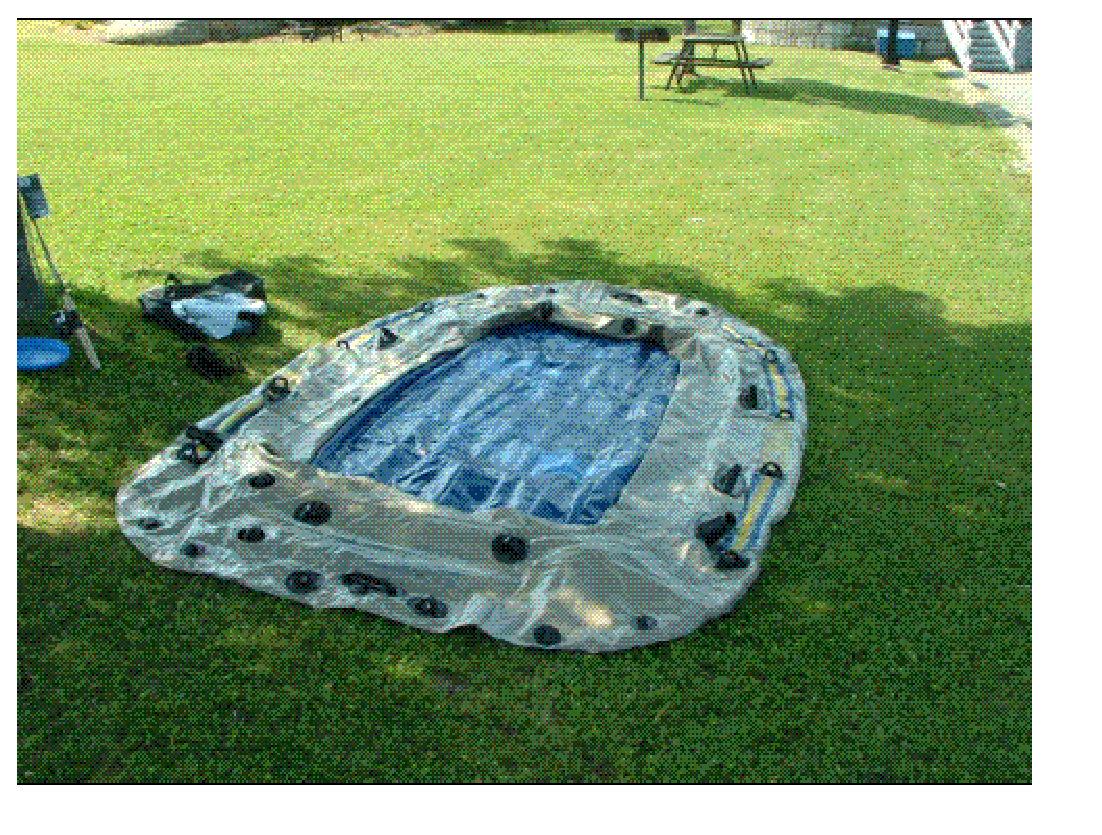
\epsfig{file=fig1.eps,width=3.5in}
Which one of the following is missing in it?
  
  
\noindent\hspace{3.0in} \begin{tabular}{|l|}
\hline
Your choice \\
\hline
 \\ 
 \\ 
\hline
\end{tabular}
  
  
 
 
\noindent{\textbf{\large{
A.}}}
Lawn
 
 
\noindent{\textbf{\large{
B.}}}
A table
 
 
\noindent{\textbf{\large{
C.}}}
A truck
 
 
\noindent{\textbf{\large{
D.}}}
An airplane
 
 
\noindent{\textbf{\large{
E.}}}
A frisbee
 
 
\noindent{\textbf{\large{
F.}}}
  Not any of aboves.
 
 
 
\vspace{0.3in}
  
\vspace{0.2in}
  
         \begin{tabular}{|l|}
\hline
 Your marks  \\
\hline
 \\ 
 \\ 
\hline
\end{tabular}
\hspace{0.05in} \begin{tabular}{|l|}
\hline
 Full marks  \\
\hline
 \\ 
12.50 \\
\hline
\end{tabular}
{\textbf{\Large{Question
30.1.6 
}}}
  
  
What is the operation between $a= % 
5$ and $b= % 
2$:
$a$  % 
$+$ $b=?$ Please also calculate it.

 
\vspace{0.3in}
   
   
\vspace{0.3in}
{\textbf{\LARGE{You have done all the above? A very good beginning, please go ahead.}}}
More constants the
Mass of electron
$m_e$$ =
9.109390 \times 10^{-31} $
kg
,
Universal gas constant
$R$$ =
8.315 $
J/(mol$\cdot $K)
,
$e$$ =
1.60217733 \times 10^{-19} $
C
, and
$m_p$$ =
1.6726231 \times 10^{-27} $
kg
%
may be very helpful.
\vspace{0.3in}
   
   
  
\vspace{0.2in}
  
\noindent\begin{tabular}{|l|}
\hline
 YOUR MARKS  \\
\hline
 \\ 
 \\ 
\hline
\end{tabular}
\hspace{0.05in} \begin{tabular}{|l|}
\hline
 Full Marks  \\
\hline
 \\ 
3.13 \\
\hline
\end{tabular}
{\textbf{\Large{QUESTION
30.2 
}}}
  
  
Considering case-insensitivity, please match the following same strings.
  
  
\begin{tabular}{|l|l|l|}
 \hline
 Column Left & Column Right  & Your choinces \\ 
 \hline
{\textbf{\large{
A.}}}
C
  & 
YJH
 & 
 \\ 
 \hline
{\textbf{\large{
B.}}}
er
  & 
ER
 & 
 \\ 
 \hline
{\textbf{\large{
C.}}}
Er
  & 
c
 & 
 \\ 
 \hline
{\textbf{\large{
D.}}}
yjh
  & 
 a= %
3
 & 
 \\ 
 \hline
{\textbf{\large{
E.}}}
 A= %
6/ %
2

  & 
eR
 & 
 \\ 
 \hline
 \end{tabular}
  
  
 
  
\vspace{0.2in}
  
\noindent\begin{tabular}{|l|}
\hline
 YOUR MARKS  \\
\hline
 \\ 
 \\ 
\hline
\end{tabular}
\hspace{0.05in} \begin{tabular}{|l|}
\hline
 Full Marks  \\
\hline
 \\ 
1.56 \\
\hline
\end{tabular}
{\textbf{\Large{QUESTION
30.3 
}}}
  
  
Please choose the correct one from the following statements:
  
  
\noindent\hspace{3.0in} \begin{tabular}{|l|}
\hline
Your choice \\
\hline
 \\ 
 \\ 
\hline
\end{tabular}
  
  
 
 
\noindent{\textbf{\large{
A.}}}
Canada has  %
36 provinces and  %
35 territories.
 
 
\noindent{\textbf{\large{
B.}}}
Canada has  %
10 provinces and  %
3 territories.
 
 
\noindent{\textbf{\large{
C.}}}
Canada has  %
34 provinces and  %
39 territories.
 
 
\noindent{\textbf{\large{
D.}}}
Canada has  %
37 provinces and  %
37 territories.
 
 
\noindent{\textbf{\large{
E.}}}
Canada has  %
35 provinces and  %
34 territories.
 
 
\noindent{\textbf{\large{
F.}}}
 None of above.
 
 
  
\vspace{0.2in}
  
\noindent\begin{tabular}{|l|}
\hline
 YOUR MARKS  \\
\hline
 \\ 
 \\ 
\hline
\end{tabular}
\hspace{0.05in} \begin{tabular}{|l|}
\hline
 Full Marks  \\
\hline
 \\ 
3.13 \\
\hline
\end{tabular}
{\textbf{\Large{QUESTION
30.4 
}}}
  
  
 
 
An object is subjected to an external net force $\mathbf{f}=
(30.0 , 8.0 , -7000.0) N$.
Its mass is known as $m= % 
56.0000 kg$. Please choose the
correct accelaration from the following choices.
 
  
  
\noindent\hspace{3.0in} \begin{tabular}{|l|}
\hline
Your choice \\
\hline
 \\ 
 \\ 
\hline
\end{tabular}
  
  
 
 
\noindent{\textbf{\large{
A.}}}
The accelaration is $  %
(
-3.63,
-.69,
-125.00)
ms^{-2} $.
 
 
\noindent{\textbf{\large{
B.}}}
The accelaration is $  %
(
-3.63,
.14,
-125.00)
ms^{-2} $.
 
 
\noindent{\textbf{\large{
C.}}}
The accelaration is $  %
(
-3.63,
-.69,
570.50)
ms^{-2} $.
 
 
\noindent{\textbf{\large{
D.}}}
The accelaration is $  %
(
.536,
-.69,
570.50)
ms^{-2} $.
 
 
\noindent{\textbf{\large{
E.}}}
The accelaration is $  %
(
.536,
.14,
-125.00)
ms^{-2} $.
 
 
\noindent{\textbf{\large{
F.}}}
The accelaration is $  %
(
.536,
.14,
570.50)
ms^{-2} $.
 
 
\noindent{\textbf{\large{
G.}}}
The accelaration is $  %
(
-3.63,
.14,
570.50)
ms^{-2} $.
 
 
\noindent{\textbf{\large{
H.}}}
The accelaration is $  %
(
.536,
-.69,
-125.00)
ms^{-2} $.
 
 
 

 

 
\vspace{0.3in}
  
\vspace{0.2in}
  
\noindent\begin{tabular}{|l|}
\hline
 YOUR MARKS  \\
\hline
 \\ 
 \\ 
\hline
\end{tabular}
\hspace{0.05in} \begin{tabular}{|l|}
\hline
 Full Marks  \\
\hline
 \\ 
1.56 \\
\hline
\end{tabular}
{\textbf{\Large{QUESTION
30.5 
}}}
  
  
If any one of the following statements is correct, please fill the box ahead of it with $T$ .
If wrong, fill with $F$.
 
\noindent\begin{tabular}{|l|l|}\hline Your&\hspace{.2in} \\ answer&\hspace{.2in} \\ \hline \end{tabular}
1. $ % 
28$ is an  % 
even number.
 
\noindent\begin{tabular}{|l|l|}\hline Your&\hspace{.2in} \\ answer&\hspace{.2in} \\ \hline \end{tabular}
2.  % 
Montreal is in  % 
Quebec province.
 
\noindent\begin{tabular}{|l|l|}\hline Your&\hspace{.2in} \\ answer&\hspace{.2in} \\ \hline \end{tabular}
3.  % 
$\mathbf{F}=m\mathbf{a}$ is a mathmatical form of
the Newton's Second Law.
 

 
\vspace{0.3in}
  
\vspace{0.2in}
  
\noindent\begin{tabular}{|l|}
\hline
 YOUR MARKS  \\
\hline
 \\ 
 \\ 
\hline
\end{tabular}
\hspace{0.05in} \begin{tabular}{|l|}
\hline
 Full Marks  \\
\hline
 \\ 
1.56 \\
\hline
\end{tabular}
{\textbf{\Large{QUESTION
30.6 
}}}
  
  
 
An object is subjected to an external net force $\mathbf{f}=(
80.000 ,
5.0000,
-9000.0  )N$. Its mass is known as
$m= % 
54.0000  kg$. Please choose the correct accelaration
from the following choices.
 
  
  
\noindent\hspace{3.0in} \begin{tabular}{|l|}
\hline
Your choice \\
\hline
 \\ 
 \\ 
\hline
\end{tabular}
  
  
 
 
\noindent{\textbf{\large{
A.}}}
The accelaration is
$(
5.6440ms^{-2},
-3602.7km/h^2,
-166.67ms^{-2}
).
$
 
 
\noindent{\textbf{\large{
B.}}}
The accelaration is
$(
1.4815ms^{-2},
1200.0km/h^2,
-166.67ms^{-2}
).
$
 
 
\noindent{\textbf{\large{
C.}}}
The accelaration is
$(
1.4815ms^{-2},
1200.0km/h^2,
-709.22ms^{-2}
).
$
 
 
\noindent{\textbf{\large{
D.}}}
The accelaration is
$(
5.6440ms^{-2},
-3602.7km/h^2,
-709.22ms^{-2}
).
$
 
 
\noindent{\textbf{\large{
E.}}}
The accelaration is
$(
1.4815ms^{-2},
-3602.7km/h^2,
-166.67ms^{-2}
).
$
 
 
\noindent{\textbf{\large{
F.}}}
The accelaration is
$(
1.4815ms^{-2},
-3602.7km/h^2,
-709.22ms^{-2}
).
$
 
 
\noindent{\textbf{\large{
G.}}}
 None of these.
 
 
 
 

 
\vspace{0.3in}
   
   
\vspace{0.3in}
{\textbf{\LARGE{You have done all the above? Excellent! Not much left, please continue.}}}
\vspace{0.3in}
   
   
  
\vspace{0.2in}
  
\noindent\begin{tabular}{|l|}
\hline
 YOUR MARKS  \\
\hline
 \\ 
 \\ 
\hline
\end{tabular}
\hspace{0.05in} \begin{tabular}{|l|}
\hline
 Full Marks  \\
\hline
 \\ 
12.50 \\
\hline
\end{tabular}
{\textbf{\Large{QUESTION
30.7 
}}}
  
  
 
$ \left( \begin{array}{ccccccccc}
           7 & 
           4 & 
           5 & 
           7 \\ 
           4 & 
           5 & 
           6 & 
           4 \\ 
           7 & 
           5 & 
           5 & 
           7
\end{array}\right) \times
\left( \begin{array}{c}
           2 \\ 
           2 \\ 
           2 \\ 
           2
\end{array}\right) $ =?
 
 
$  % 
 \left( \begin{array}
 {
 c
 c
 }
 \rho & 
 \beta \\ 
                    \zeta & 
 \Theta \\ 
 \Lambda & 
 \Psi \\ 
 \Gamma & 
 \Gamma
 \end{array} \right)
 \left( \begin{array}
 {
 c
 }
 \beta \\ 
 \beta
 \end{array} \right)
$ =?
 

 

 
\vspace{0.3in}
  
\vspace{0.2in}
  
\noindent\begin{tabular}{|l|}
\hline
 YOUR MARKS  \\
\hline
 \\ 
 \\ 
\hline
\end{tabular}
\hspace{0.05in} \begin{tabular}{|l|}
\hline
 Full Marks  \\
\hline
 \\ 
12.50 \\
\hline
\end{tabular}
{\textbf{\Large{QUESTION
30.8 
}}}
  
  
 
An object is subjected to an external net force $\mathbf{f}=
(90.0 , 2.0 , -6000.0) N$.
Its mass is known as $m= % 
54.0 kg$.
Please choose the correct accelaration from the following choices.
  
  
\noindent\hspace{3.0in} \begin{tabular}{|l|}
\hline
Your choice \\
\hline
 \\ 
 \\ 
\hline
\end{tabular}
  
  
 
 
\noindent{\textbf{\large{
A.}}}
  The accelaration is $  %
(
-8.24,
.17,
-111.11)
ms^{-2} $.
 
 
\noindent{\textbf{\large{
B.}}}
  The accelaration is $  %
(
-8.24,
3.7 \times 10^{-2},
351.37)
ms^{-2} $.
 
 
\noindent{\textbf{\large{
C.}}}
  The accelaration is $  %
(
1.67,
3.7 \times 10^{-2},
-111.11)
ms^{-2} $.
 
 
\noindent{\textbf{\large{
D.}}}
  The accelaration is $  %
(
-8.24,
.17,
351.37)
ms^{-2} $.
 
 
 

 
 
\vspace{0.3in}
  
\vspace{0.2in}
  
\noindent\begin{tabular}{|l|}
\hline
 YOUR MARKS  \\
\hline
 \\ 
 \\ 
\hline
\end{tabular}
\hspace{0.05in} \begin{tabular}{|l|}
\hline
 Full Marks  \\
\hline
 \\ 
1.56 \\
\hline
\end{tabular}
{\textbf{\Large{QUESTION
30.9 
}}}
  
  
 
 
% First root
% Second root

 
Please solve the following equation:
\begin{eqnarray*}
-15 \times x^2  % 
-30
                 \times x    % 
+  % 
525 =0
\end{eqnarray*}
 

 

 
\vspace{0.3in}
   
   
 \vspace{0.2in}
Here are still some constants for use:
 
 
\noindent\begin{tabular}{|l|l|l|}
\hline
Constant & Symbol & Value \\
\hline
 
Mass of proton &
$m_p$ &
 $ 1.6726231 \times 10^{-27} $
kg \\
\hline
 
Boltzmann's constant &
$k$ &
 $ 1.381 \times 10^{-23} $
J/K \\
\hline
 
\end{tabular}
 
Thank you very much for answering these questions!
 
{\textbf{\large{Please be advised}}} that in this paper there are questions from
30.1 through
30.9.
And any one of them may contain more than one sub-question, thus the total number
of sub-questions here is around 14, of which
13 should be answered.
 
   
   
   
   
\vspace{1.0in} 
{\textbf{\large{ *** END OF PAPER, THANKS *** }}} 
   
   
\hspace{1.0in} By: 
         239(         26,          34)
   
   
   
   
\newpage 
\setcounter{page}{ 
    31001 } 
   
   
   
   
\noindent\begin{tabular}{|l|}
\hline
YOUR NAME (FIRST, ... LAST)  \\
\hline
 \\ 
 \\ 
\hline
\end{tabular}
\hspace{0.05in} \begin{tabular}{|l|}
\hline
 YOUR   ID   INFORMATION  \\
\hline
 \\ 
 \\ 
\hline
\end{tabular}
   
   
\vspace{0.2in}\noindent\begin{tabular}{|l|}
\hline
YOUR TOTAL MARKS  \\
\hline
 \\ 
 \\ 
\hline
\end{tabular}
\hspace{0.05in} \begin{tabular}{|l|}
\hline
TOTAL FULL MARKS  \\
\hline
 \\ 
100.00 \\
\hline
\end{tabular}
   
   
 \vspace{0.2in}
 
 
{\Huge  THIS IS AN EXAMPLE OF}
 
{\Huge  PERSONALIZED TESTS. }
 
If needed, please use the following constants.
 
 
 
\noindent\begin{tabular}{|l|l|l|}
\hline
Constant & Symbol & Value \\
\hline
Acceleration due to earth's gravity &
$g$ &
 $ 9.80 $
m/s$^2$ \\
\hline
Avogadro's number &
$N_A$ &
 $ 6.0221367 \times 10^{23} $
mol$^{-1}$ \\
\hline
Boltzmann's constant &
$k$ &
 $ 1.380658 \times 10^{-23} $
J/K \\
\hline
Coulomb's constant &
$k$ &
 $ 8.99 \times 10^{9} $
N$\cdot $m$^2$/C$^2$ \\
\hline
Electron charge magnitiude &
$e$ &
 $ 1.60217733 \times 10^{-19} $
C \\
\hline
Permeability of free space &
$\mu _0$ &
 $ 1.25663706 \times 10^{-6} $
T$\cdot $m/A \\
\hline
Permittivity of free space &
$\epsilon _0$ &
 $ 8.854187817 \times 10^{-12} $
C$^2$/(N$\cdot $m$^2$) \\
\hline
Pi &
$\pi$ &
 $ 3.14159265 $
$ $ \\
\hline
Planck's constant &
$h$ &
 $ 6.6260755 \times 10^{-34} $
J$\cdot $s \\
\hline
Mass of electron &
$m_e$ &
 $ 9.1093897 \times 10^{-31} $
kg \\
\hline
\end{tabular}
 
 
\noindent\begin{tabular}{|l|l|l|}
\hline
Constant & Symbol & Value \\
\hline
Mass of neutron &
$m_n$ &
 $ 1.6749286 \times 10^{-27} $
kg \\
\hline
Mass of proton &
$m_p$ &
 $ 1.6726231 \times 10^{-27} $
kg \\
\hline
Speed of light in vacuum &
$c$ &
 $ 299792458. $
m/s \\
\hline
Universal gravitational constant &
$G$ &
 $ 6.67259 \times 10^{-11} $
N$\cdot $m$^2$/kg$^2$ \\
\hline
Universal gas constant &
$R$ &
 $ 8.314510 $
J/(mol$\cdot $K) \\
\hline
\end{tabular}
 
 
{\textbf{\large{Please be advised}}} that in this paper there are questions from
31.1 through
31.9.
And any one of them may contain more than one sub-question, thus the total number
of sub-questions here is around 14, of which
13 should be answered.
 
\vspace{0.3in}
 
 
   
   
  
\vspace{0.2in}
  
\noindent\begin{tabular}{|l|}
\hline
 YOUR MARKS  \\
\hline
 \\ 
 \\ 
\hline
\end{tabular}
\hspace{0.05in} \begin{tabular}{|l|}
\hline
 Full Marks  \\
\hline
 \\ 
62.50 \\
\hline
\end{tabular}
{\textbf{\Large{QUESTION
31.1 
}}}
  
  
 
{\textbf{\Large{Please answer ONLY
5 of the following
6 questions (Questions
31.1.1 through
31.1.6). }}}
 
Here are still some constants for use in the following questions:
 
 
\noindent\begin{tabular}{|l|l|l|}
\hline
Constant & Symbol & Value \\
\hline
 
Boltzmann's constant &
$k$ &
 $ 1.381 \times 10^{-23} $
J/K \\
\hline
 
Avogadro's number &
$N_A$ &
 $ 6.022 \times 10^{23} $
mol$^{-1}$ \\
\hline
 
Mass of electron &
$m_e$ &
 $ 9.1093897 \times 10^{-31} $
kg \\
\hline
 
\end{tabular}
 
  
\vspace{0.2in}
  
         \begin{tabular}{|l|}
\hline
 Your marks  \\
\hline
 \\ 
 \\ 
\hline
\end{tabular}
\hspace{0.05in} \begin{tabular}{|l|}
\hline
 Full marks  \\
\hline
 \\ 
12.50 \\
\hline
\end{tabular}
{\textbf{\Large{Question
31.1.1 
}}}
  
  
Let us use Newton's Law of Universal Gravitation to calculate the force
of the Sun acting on the eight planets. Let us suppose the mass of the
Sun is $ % 
5.00 \times 10^{24} kg$. With the mass and the
distance to the Sun of each planet in the following table, please fill
the blanks for the forces.
 
\vspace{0.2in}
 
 
\begin{tabular}{|l|l|l|l|}
\hline
The Planet & Mass ($kg$) & Distanace from Sun ($m$) & The Force ($N$)\\
\hline
Mercury  &
           $ % 
7.00000000 \times 10^{24} $   &
             $ % 
5.000000000 \times 10^{24} $    &
\\  \hline
Venus    &
           $ % 
2.00 \times 10^{24} $    &
             $ % 
6.00 \times 10^{24} $    &
\\  \hline
Earth    &
           $ % 
9.00 \times 10^{24} $    &
             $ % 
6.00 \times 10^{24} $    &
\\   \hline
Mars     &
           $ % 
2.00 \times 10^{24} $    &
             $ % 
5.00 \times 10^{24} $    &
\\   \hline
Jupiter  &
           $ % 
5.00 \times 10^{24} $    &
             $ % 
5.00 \times 10^{24} $    &
\\  \hline
Saturn   &
           $ % 
4.00 \times 10^{24}$    &
             $ % 
2.00 \times 10^{24}$    &
\\  \hline
Uranus   &
           $ % 
7.00 \times 10^{24} $    &
             $ % 
2.00 \times 10^{24} $    &
\\  \hline
Neptune  &
           $ % 
4.00 \times 10^{24} $    &
             $ % 
4.00 \times 10^{24} $    &
\\  \hline
 
\end{tabular}
 
 

 
 

 
\vspace{0.3in}
  
\vspace{0.2in}
  
         \begin{tabular}{|l|}
\hline
 Your marks  \\
\hline
 \\ 
 \\ 
\hline
\end{tabular}
\hspace{0.05in} \begin{tabular}{|l|}
\hline
 Full marks  \\
\hline
 \\ 
12.50 \\
\hline
\end{tabular}
{\textbf{\Large{Question
31.1.2 
}}}
  
  
What is the operation between $a= % 
7$ and $b= % 
2$:
$a$  % 
$-$ $b=?$ Please also calculate it.

 
\vspace{0.3in}
  
\vspace{0.2in}
  
         \begin{tabular}{|l|}
\hline
 Your marks  \\
\hline
 \\ 
 \\ 
\hline
\end{tabular}
\hspace{0.05in} \begin{tabular}{|l|}
\hline
 Full marks  \\
\hline
 \\ 
12.50 \\
\hline
\end{tabular}
{\textbf{\Large{Question
31.1.3 
}}}
  
  
In a hotel, the possiblity of  % 
smoking customer is
$a =  % 
.970$, and the possiblity of  % 
equal or above 30 years old customer is $ b =  % 
6.00 \times 10^{-2}$.
Please calculate the possiblity of  % 
 non-smoking and  % 
under 30 years old customer.
 

 

 
\vspace{0.3in}
  
\vspace{0.2in}
  
         \begin{tabular}{|l|}
\hline
 Your marks  \\
\hline
 \\ 
 \\ 
\hline
\end{tabular}
\hspace{0.05in} \begin{tabular}{|l|}
\hline
 Full marks  \\
\hline
 \\ 
12.50 \\
\hline
\end{tabular}
{\textbf{\Large{Question
31.1.4 
}}}
  
  
 
An object is subjected to an external net force $\mathbf{f}=(
40.0 ,
8.0,
-2000.0  )N$. Its mass is known as
$m= % 
58.0  kg$. Please choose the correct accelaration
from the following choices.
 
  
  
\noindent\hspace{3.0in} \begin{tabular}{|l|}
\hline
Your choice \\
\hline
 \\ 
 \\ 
\hline
\end{tabular}
  
  
 
 
\noindent{\textbf{\large{
A.}}}
The accelaration (vector) is
$(
41249.,
1787.6 ,
-1.0404 \times 10^{6}
)km/h^2.
$
 
 
\noindent{\textbf{\large{
B.}}}
The accelaration (vector) is
$(
41249.,
1787.6 ,
-446897.
)km/h^2.
$
 
 
\noindent{\textbf{\large{
C.}}}
The accelaration (vector) is
$(
32375.,
1787.6 ,
2.2177 \times 10^{6}
)km/h^2.
$
 
 
\noindent{\textbf{\large{
D.}}}
The accelaration (vector) is
$(
8937.9,
1787.6 ,
-446897.
)km/h^2.
$
 
 
\noindent{\textbf{\large{
E.}}}
The accelaration (vector) is
$(
8937.9,
1787.6 ,
2.2177 \times 10^{6}
)km/h^2.
$
 
 
\noindent{\textbf{\large{
F.}}}
The accelaration (vector) is
$(
41249.,
1787.6 ,
-1.7821 \times 10^{6}
)km/h^2.
$
 
 
\noindent{\textbf{\large{
G.}}}
The accelaration (vector) is
$(
8937.9,
1787.6 ,
-1.7821 \times 10^{6}
)km/h^2.
$
 
 
\noindent{\textbf{\large{
H.}}}
The accelaration (vector) is
$(
-41516.,
1787.6 ,
-1.0404 \times 10^{6}
)km/h^2.
$
 
 
\noindent{\textbf{\large{
I.}}}
The accelaration (vector) is
$(
32375.,
1787.6 ,
-446897.
)km/h^2.
$
 
 
\noindent{\textbf{\large{
J.}}}
The accelaration (vector) is
$(
8937.9,
1787.6 ,
-1.0404 \times 10^{6}
)km/h^2.
$
 
 
\noindent{\textbf{\large{
K.}}}
The accelaration (vector) is
$(
32375.,
1787.6 ,
-1.0404 \times 10^{6}
)km/h^2.
$
 
 
\noindent{\textbf{\large{
L.}}}
The accelaration (vector) is
$(
41249.,
1787.6 ,
2.2177 \times 10^{6}
)km/h^2.
$
 
 
 
 

 
 
\vspace{0.3in}
  
\vspace{0.2in}
  
         \begin{tabular}{|l|}
\hline
 Your marks  \\
\hline
 \\ 
 \\ 
\hline
\end{tabular}
\hspace{0.05in} \begin{tabular}{|l|}
\hline
 Full marks  \\
\hline
 \\ 
12.50 \\
\hline
\end{tabular}
{\textbf{\Large{Question
31.1.5 
}}}
  
  
 
An object is subjected to an external net force $\mathbf{f}=(
90.0 ,
9.0,
-3000.0  )N$. Its mass is known as
$m= % 
52.0  kg$. Please choose the correct accelaration
from the following choices.
 
  
  
\noindent\hspace{3.0in} \begin{tabular}{|l|}
\hline
Your choice \\
\hline
 \\ 
 \\ 
\hline
\end{tabular}
  
  
 
 
\noindent{\textbf{\large{
A.}}}
The accelaration is
$(
1.7308ms^{-2},
.17308ms^{-2},
-747692.km/h^2
).
$
 
 
\noindent{\textbf{\large{
B.}}}
The accelaration is
$(
5.8592ms^{-2},
.17308ms^{-2},
-747692.km/h^2
).
$
 
 
\noindent{\textbf{\large{
C.}}}
The accelaration is
$(
5.8592ms^{-2},
.74216ms^{-2},
-747692.km/h^2
).
$
 
 
\noindent{\textbf{\large{
D.}}}
The accelaration is
$(
5.8592ms^{-2},
.74216ms^{-2},
3.4579 \times 10^{6}km/h^2
).
$
 
 
\noindent{\textbf{\large{
E.}}}
none of these.
 
 
 
 

 
\vspace{0.3in}
  
\vspace{0.2in}
  
         \begin{tabular}{|l|}
\hline
 Your marks  \\
\hline
 \\ 
 \\ 
\hline
\end{tabular}
\hspace{0.05in} \begin{tabular}{|l|}
\hline
 Full marks  \\
\hline
 \\ 
12.50 \\
\hline
\end{tabular}
{\textbf{\Large{Question
31.1.6 
}}}
  
  
In a hotel, the possiblity of  % 
smoking customer is
$a =  % 
.470$, and the possiblity of  % 
equal-or-above 30 years old customer is $ b =  % 
.1600$.
Please fill the following form.
 
\noindent
\begin{tabular}{|l|l|}
\hline
Customer & Possibility \\
\hline
smoking  and   % 
equal-or-above 30 years old  & \\
\hline
smoking  and   % 
under 30 years old & \\
\hline
 non-smoking and   % 
equal-or-above 30 years old  & \\
\hline
 non-smoking and  % 
under 30 years old & \\
\hline
\end{tabular}
 
 
 

 

 
\vspace{0.3in}
   
   
\vspace{0.3in}
{\textbf{\LARGE{You have done all the above? A very good beginning, please go ahead.}}}
More constants the
Mass of electron
$m_e$$ =
9.109390 \times 10^{-31} $
kg
,
Universal gas constant
$R$$ =
8.315 $
J/(mol$\cdot $K)
,
$e$$ =
1.60217733 \times 10^{-19} $
C
, and
$m_p$$ =
1.6726231 \times 10^{-27} $
kg
%
may be very helpful.
\vspace{0.3in}
   
   
  
\vspace{0.2in}
  
\noindent\begin{tabular}{|l|}
\hline
 YOUR MARKS  \\
\hline
 \\ 
 \\ 
\hline
\end{tabular}
\hspace{0.05in} \begin{tabular}{|l|}
\hline
 Full Marks  \\
\hline
 \\ 
1.56 \\
\hline
\end{tabular}
{\textbf{\Large{QUESTION
31.2 
}}}
  
  
Please choose the correct one from the following statements:
  
  
\noindent\hspace{3.0in} \begin{tabular}{|l|}
\hline
Your choice \\
\hline
 \\ 
 \\ 
\hline
\end{tabular}
  
  
 
 
\noindent{\textbf{\large{
A.}}}
Canada has  %
33 provinces and  %
38 territories.
 
 
\noindent{\textbf{\large{
B.}}}
Canada has  %
37 provinces and  %
37 territories.
 
 
\noindent{\textbf{\large{
C.}}}
Canada has  %
34 provinces and  %
39 territories.
 
 
\noindent{\textbf{\large{
D.}}}
Canada has  %
10 provinces and  %
3 territories.
 
 
\noindent{\textbf{\large{
E.}}}
Canada has  %
36 provinces and  %
35 territories.
 
 
\noindent{\textbf{\large{
F.}}}
 None of above.
 
 
  
\vspace{0.2in}
  
\noindent\begin{tabular}{|l|}
\hline
 YOUR MARKS  \\
\hline
 \\ 
 \\ 
\hline
\end{tabular}
\hspace{0.05in} \begin{tabular}{|l|}
\hline
 Full Marks  \\
\hline
 \\ 
3.13 \\
\hline
\end{tabular}
{\textbf{\Large{QUESTION
31.3 
}}}
  
  
Considering case-insensitivity, please match the following same strings.
  
  
\begin{tabular}{|l|l|l|}
 \hline
 Column Left & Column Right  & Your choinces \\ 
 \hline
{\textbf{\large{
A.}}}
yjh
  & 
b
 & 
 \\ 
 \hline
{\textbf{\large{
B.}}}
B
  & 
ER
 & 
 \\ 
 \hline
{\textbf{\large{
C.}}}
Er
  & 
 a= %
2
 & 
 \\ 
 \hline
{\textbf{\large{
D.}}}
A
  & 
YJH
 & 
 \\ 
 \hline
{\textbf{\large{
E.}}}
 A= %
4/ %
2

  & 
a
 & 
 \\ 
 \hline
 \end{tabular}
  
  
 
  
\vspace{0.2in}
  
\noindent\begin{tabular}{|l|}
\hline
 YOUR MARKS  \\
\hline
 \\ 
 \\ 
\hline
\end{tabular}
\hspace{0.05in} \begin{tabular}{|l|}
\hline
 Full Marks  \\
\hline
 \\ 
1.56 \\
\hline
\end{tabular}
{\textbf{\Large{QUESTION
31.4 
}}}
  
  
 
An object is subjected to an external net force $\mathbf{f}=(
60.000 ,
5.0000,
-6000.0  )N$. Its mass is known as
$m= % 
50.0000  kg$. Please choose the correct accelaration
from the following choices.
 
  
  
\noindent\hspace{3.0in} \begin{tabular}{|l|}
\hline
Your choice \\
\hline
 \\ 
 \\ 
\hline
\end{tabular}
  
  
 
 
\noindent{\textbf{\large{
A.}}}
The accelaration is
$(
1.2000ms^{-2},
5760.2km/h^2,
-120.00ms^{-2}
).
$
 
 
\noindent{\textbf{\large{
B.}}}
The accelaration is
$(
1.2000ms^{-2},
1296.0km/h^2,
-120.00ms^{-2}
).
$
 
 
\noindent{\textbf{\large{
C.}}}
The accelaration is
$(
-3.1540ms^{-2},
1296.0km/h^2,
-120.00ms^{-2}
).
$
 
 
\noindent{\textbf{\large{
D.}}}
The accelaration is
$(
-3.1540ms^{-2},
5760.2km/h^2,
478.93ms^{-2}
).
$
 
 
\noindent{\textbf{\large{
E.}}}
The accelaration is
$(
1.2000ms^{-2},
5760.2km/h^2,
478.93ms^{-2}
).
$
 
 
\noindent{\textbf{\large{
F.}}}
The accelaration is
$(
-3.1540ms^{-2},
5760.2km/h^2,
-120.00ms^{-2}
).
$
 
 
\noindent{\textbf{\large{
G.}}}
 None of these.
 
 
 
 

 
\vspace{0.3in}
  
\vspace{0.2in}
  
\noindent\begin{tabular}{|l|}
\hline
 YOUR MARKS  \\
\hline
 \\ 
 \\ 
\hline
\end{tabular}
\hspace{0.05in} \begin{tabular}{|l|}
\hline
 Full Marks  \\
\hline
 \\ 
1.56 \\
\hline
\end{tabular}
{\textbf{\Large{QUESTION
31.5 
}}}
  
  
If any one of the following statements is correct, please fill the box ahead of it with $T$ .
If wrong, fill with $F$.
 
\noindent\begin{tabular}{|l|l|}\hline Your&\hspace{.2in} \\ answer&\hspace{.2in} \\ \hline \end{tabular}
1. $ % 
37$ is an  % 
even number.
 
\noindent\begin{tabular}{|l|l|}\hline Your&\hspace{.2in} \\ answer&\hspace{.2in} \\ \hline \end{tabular}
2.  % 
Hull is in  % 
Ontario province.
 
\noindent\begin{tabular}{|l|l|}\hline Your&\hspace{.2in} \\ answer&\hspace{.2in} \\ \hline \end{tabular}
3.  % 
$\mathbf{F}=m\mathbf{a}$ is a mathmatical form of
Newton's Law of Universal Gravitation.
 

 
\vspace{0.3in}
  
\vspace{0.2in}
  
\noindent\begin{tabular}{|l|}
\hline
 YOUR MARKS  \\
\hline
 \\ 
 \\ 
\hline
\end{tabular}
\hspace{0.05in} \begin{tabular}{|l|}
\hline
 Full Marks  \\
\hline
 \\ 
3.13 \\
\hline
\end{tabular}
{\textbf{\Large{QUESTION
31.6 
}}}
  
  
 
 
An object is subjected to an external net force $\mathbf{f}=
(50.0 , 5.0 , -9000.0) N$.
Its mass is known as $m= % 
56.0000 kg$. Please choose the
correct accelaration from the following choices.
 
  
  
\noindent\hspace{3.0in} \begin{tabular}{|l|}
\hline
Your choice \\
\hline
 \\ 
 \\ 
\hline
\end{tabular}
  
  
 
 
\noindent{\textbf{\large{
A.}}}
The accelaration is $  %
(
.893,
-.27,
-456.38)
ms^{-2} $.
 
 
\noindent{\textbf{\large{
B.}}}
The accelaration is $  %
(
4.31,
-.27,
-160.71)
ms^{-2} $.
 
 
\noindent{\textbf{\large{
C.}}}
The accelaration is $  %
(
.893,
8.9 \times 10^{-2},
-456.38)
ms^{-2} $.
 
 
\noindent{\textbf{\large{
D.}}}
The accelaration is $  %
(
4.31,
8.9 \times 10^{-2},
-160.71)
ms^{-2} $.
 
 
\noindent{\textbf{\large{
E.}}}
The accelaration is $  %
(
.893,
8.9 \times 10^{-2},
-160.71)
ms^{-2} $.
 
 
\noindent{\textbf{\large{
F.}}}
The accelaration is $  %
(
4.31,
8.9 \times 10^{-2},
-456.38)
ms^{-2} $.
 
 
\noindent{\textbf{\large{
G.}}}
The accelaration is $  %
(
4.31,
-.27,
-456.38)
ms^{-2} $.
 
 
\noindent{\textbf{\large{
H.}}}
The accelaration is $  %
(
.893,
-.27,
-160.71)
ms^{-2} $.
 
 
 

 

 
\vspace{0.3in}
   
   
\vspace{0.3in}
{\textbf{\LARGE{You have done all the above? Excellent! Not much left, please continue.}}}
\vspace{0.3in}
   
   
  
\vspace{0.2in}
  
\noindent\begin{tabular}{|l|}
\hline
 YOUR MARKS  \\
\hline
 \\ 
 \\ 
\hline
\end{tabular}
\hspace{0.05in} \begin{tabular}{|l|}
\hline
 Full Marks  \\
\hline
 \\ 
12.50 \\
\hline
\end{tabular}
{\textbf{\Large{QUESTION
31.7 
}}}
  
  
 
$ \left( \begin{array}{ccccccccc}
           4 & 
           6 & 
           5 & 
           6 \\ 
           5 & 
           4 & 
           5 & 
           6 \\ 
           6 & 
           5 & 
           5 & 
           5
\end{array}\right) \times
\left( \begin{array}{c}
           2 \\ 
           2 \\ 
           2 \\ 
           2
\end{array}\right) $ =?
 
 
$  % 
 \left( \begin{array}
 {
 c
 c
 }
 \Phi & 
 \gamma \\ 
 \Upsilon & 
 \Upsilon \\ 
 \beta & 
                    \zeta \\ 
 \Lambda & 
 \Delta
 \end{array} \right)
 \left( \begin{array}
 {
 c
 }
 \gamma \\ 
 \beta
 \end{array} \right)
$ =?
 

 

 
\vspace{0.3in}
  
\vspace{0.2in}
  
\noindent\begin{tabular}{|l|}
\hline
 YOUR MARKS  \\
\hline
 \\ 
 \\ 
\hline
\end{tabular}
\hspace{0.05in} \begin{tabular}{|l|}
\hline
 Full Marks  \\
\hline
 \\ 
12.50 \\
\hline
\end{tabular}
{\textbf{\Large{QUESTION
31.8 
}}}
  
  
 
An object is subjected to an external net force $\mathbf{f}=
(50.0 , 5.0 , -3000.0) N$.
Its mass is known as $m= % 
58.0 kg$.
Please choose the correct accelaration from the following choices.
  
  
\noindent\hspace{3.0in} \begin{tabular}{|l|}
\hline
Your choice \\
\hline
 \\ 
 \\ 
\hline
\end{tabular}
  
  
 
 
\noindent{\textbf{\large{
A.}}}
  The accelaration is $  %
(
-3.63,
8.6 \times 10^{-2},
-51.724)
ms^{-2} $.
 
 
\noindent{\textbf{\large{
B.}}}
  The accelaration is $  %
(
-3.63,
8.6 \times 10^{-2},
-256.91)
ms^{-2} $.
 
 
\noindent{\textbf{\large{
C.}}}
  The accelaration is $  %
(
.862,
8.6 \times 10^{-2},
-51.724)
ms^{-2} $.
 
 
\noindent{\textbf{\large{
D.}}}
  The accelaration is $  %
(
-3.63,
.41,
-256.91)
ms^{-2} $.
 
 
 

 
 
\vspace{0.3in}
  
\vspace{0.2in}
  
\noindent\begin{tabular}{|l|}
\hline
 YOUR MARKS  \\
\hline
 \\ 
 \\ 
\hline
\end{tabular}
\hspace{0.05in} \begin{tabular}{|l|}
\hline
 Full Marks  \\
\hline
 \\ 
1.56 \\
\hline
\end{tabular}
{\textbf{\Large{QUESTION
31.9 
}}}
  
  
 
 
% First root
% Second root

 
Please solve the following equation:
\begin{eqnarray*}
9 \times x^2  % 
+  % 
72
                 \times x    % 
+  % 
63 =0
\end{eqnarray*}
 

 

 
\vspace{0.3in}
   
   
 \vspace{0.2in}
Here are still some constants for use:
 
 
\noindent\begin{tabular}{|l|l|l|}
\hline
Constant & Symbol & Value \\
\hline
 
Mass of proton &
$m_p$ &
 $ 1.6726231 \times 10^{-27} $
kg \\
\hline
 
Boltzmann's constant &
$k$ &
 $ 1.381 \times 10^{-23} $
J/K \\
\hline
 
\end{tabular}
 
Thank you very much for answering these questions!
 
{\textbf{\large{Please be advised}}} that in this paper there are questions from
31.1 through
31.9.
And any one of them may contain more than one sub-question, thus the total number
of sub-questions here is around 14, of which
13 should be answered.
 
   
   
   
   
\vspace{1.0in} 
{\textbf{\large{ *** END OF PAPER, THANKS *** }}} 
   
   
\hspace{1.0in} By: 
         239(         26,          34)
   
   
   
   
\newpage 
\setcounter{page}{ 
    32001 } 
   
   
   
   
\noindent\begin{tabular}{|l|}
\hline
YOUR NAME (FIRST, ... LAST)  \\
\hline
 \\ 
 \\ 
\hline
\end{tabular}
\hspace{0.05in} \begin{tabular}{|l|}
\hline
 YOUR   ID   INFORMATION  \\
\hline
 \\ 
 \\ 
\hline
\end{tabular}
   
   
\vspace{0.2in}\noindent\begin{tabular}{|l|}
\hline
YOUR TOTAL MARKS  \\
\hline
 \\ 
 \\ 
\hline
\end{tabular}
\hspace{0.05in} \begin{tabular}{|l|}
\hline
TOTAL FULL MARKS  \\
\hline
 \\ 
100.00 \\
\hline
\end{tabular}
   
   
 \vspace{0.2in}
 
 
{\Huge  THIS IS AN EXAMPLE OF}
 
{\Huge  PERSONALIZED TESTS. }
 
If needed, please use the following constants.
 
 
 
\noindent\begin{tabular}{|l|l|l|}
\hline
Constant & Symbol & Value \\
\hline
Acceleration due to earth's gravity &
$g$ &
 $ 9.80 $
m/s$^2$ \\
\hline
Avogadro's number &
$N_A$ &
 $ 6.0221367 \times 10^{23} $
mol$^{-1}$ \\
\hline
Boltzmann's constant &
$k$ &
 $ 1.380658 \times 10^{-23} $
J/K \\
\hline
Coulomb's constant &
$k$ &
 $ 8.99 \times 10^{9} $
N$\cdot $m$^2$/C$^2$ \\
\hline
Electron charge magnitiude &
$e$ &
 $ 1.60217733 \times 10^{-19} $
C \\
\hline
Permeability of free space &
$\mu _0$ &
 $ 1.25663706 \times 10^{-6} $
T$\cdot $m/A \\
\hline
Permittivity of free space &
$\epsilon _0$ &
 $ 8.854187817 \times 10^{-12} $
C$^2$/(N$\cdot $m$^2$) \\
\hline
Pi &
$\pi$ &
 $ 3.14159265 $
$ $ \\
\hline
Planck's constant &
$h$ &
 $ 6.6260755 \times 10^{-34} $
J$\cdot $s \\
\hline
Mass of electron &
$m_e$ &
 $ 9.1093897 \times 10^{-31} $
kg \\
\hline
\end{tabular}
 
 
\noindent\begin{tabular}{|l|l|l|}
\hline
Constant & Symbol & Value \\
\hline
Mass of neutron &
$m_n$ &
 $ 1.6749286 \times 10^{-27} $
kg \\
\hline
Mass of proton &
$m_p$ &
 $ 1.6726231 \times 10^{-27} $
kg \\
\hline
Speed of light in vacuum &
$c$ &
 $ 299792458. $
m/s \\
\hline
Universal gravitational constant &
$G$ &
 $ 6.67259 \times 10^{-11} $
N$\cdot $m$^2$/kg$^2$ \\
\hline
Universal gas constant &
$R$ &
 $ 8.314510 $
J/(mol$\cdot $K) \\
\hline
\end{tabular}
 
 
{\textbf{\large{Please be advised}}} that in this paper there are questions from
32.1 through
32.9.
And any one of them may contain more than one sub-question, thus the total number
of sub-questions here is around 14, of which
13 should be answered.
 
\vspace{0.3in}
 
 
   
   
  
\vspace{0.2in}
  
\noindent\begin{tabular}{|l|}
\hline
 YOUR MARKS  \\
\hline
 \\ 
 \\ 
\hline
\end{tabular}
\hspace{0.05in} \begin{tabular}{|l|}
\hline
 Full Marks  \\
\hline
 \\ 
62.50 \\
\hline
\end{tabular}
{\textbf{\Large{QUESTION
32.1 
}}}
  
  
 
{\textbf{\Large{Please answer ONLY
5 of the following
6 questions (Questions
32.1.1 through
32.1.6). }}}
 
Here are still some constants for use in the following questions:
 
 
\noindent\begin{tabular}{|l|l|l|}
\hline
Constant & Symbol & Value \\
\hline
 
Boltzmann's constant &
$k$ &
 $ 1.381 \times 10^{-23} $
J/K \\
\hline
 
Avogadro's number &
$N_A$ &
 $ 6.022 \times 10^{23} $
mol$^{-1}$ \\
\hline
 
Mass of electron &
$m_e$ &
 $ 9.1093897 \times 10^{-31} $
kg \\
\hline
 
\end{tabular}
 
  
\vspace{0.2in}
  
         \begin{tabular}{|l|}
\hline
 Your marks  \\
\hline
 \\ 
 \\ 
\hline
\end{tabular}
\hspace{0.05in} \begin{tabular}{|l|}
\hline
 Full marks  \\
\hline
 \\ 
12.50 \\
\hline
\end{tabular}
{\textbf{\Large{Question
32.1.1 
}}}
  
  
In a hotel, the possiblity of  % 
non-smoking customer is
$a =  % 
.460$, and the possiblity of  % 
equal-or-above 30 years old customer is $ b =  % 
.7000$.
Please fill the following form.
 
\noindent
\begin{tabular}{|l|l|}
\hline
Customer & Possibility \\
\hline
smoking  and   % 
equal-or-above 30 years old  & \\
\hline
smoking  and   % 
under 30 years old & \\
\hline
 non-smoking and   % 
equal-or-above 30 years old  & \\
\hline
 non-smoking and  % 
under 30 years old & \\
\hline
\end{tabular}
 
 
 

 

 
\vspace{0.3in}
  
\vspace{0.2in}
  
         \begin{tabular}{|l|}
\hline
 Your marks  \\
\hline
 \\ 
 \\ 
\hline
\end{tabular}
\hspace{0.05in} \begin{tabular}{|l|}
\hline
 Full marks  \\
\hline
 \\ 
12.50 \\
\hline
\end{tabular}
{\textbf{\Large{Question
32.1.2 
}}}
  
  
 
An object is subjected to an external net force $\mathbf{f}=(
90.0 ,
5.0,
-5000.0  )N$. Its mass is known as
$m= % 
54.0  kg$. Please choose the correct accelaration
from the following choices.
 
  
  
\noindent\hspace{3.0in} \begin{tabular}{|l|}
\hline
Your choice \\
\hline
 \\ 
 \\ 
\hline
\end{tabular}
  
  
 
 
\noindent{\textbf{\large{
A.}}}
The accelaration is
$(
5.4286ms^{-2},
.41036ms^{-2},
-1.2000 \times 10^{6}km/h^2
).
$
 
 
\noindent{\textbf{\large{
B.}}}
The accelaration is
$(
5.4286ms^{-2},
.41036ms^{-2},
2.5023 \times 10^{6}km/h^2
).
$
 
 
\noindent{\textbf{\large{
C.}}}
The accelaration is
$(
1.6667ms^{-2},
9.2593 \times 10^{-2}ms^{-2},
-1.2000 \times 10^{6}km/h^2
).
$
 
 
\noindent{\textbf{\large{
D.}}}
The accelaration is
$(
5.4286ms^{-2},
9.2593 \times 10^{-2}ms^{-2},
2.5023 \times 10^{6}km/h^2
).
$
 
 
\noindent{\textbf{\large{
E.}}}
none of these.
 
 
 
 

 
\vspace{0.3in}
  
\vspace{0.2in}
  
         \begin{tabular}{|l|}
\hline
 Your marks  \\
\hline
 \\ 
 \\ 
\hline
\end{tabular}
\hspace{0.05in} \begin{tabular}{|l|}
\hline
 Full marks  \\
\hline
 \\ 
12.50 \\
\hline
\end{tabular}
{\textbf{\Large{Question
32.1.3 
}}}
  
  
Let us use Newton's Law of Universal Gravitation to calculate the force
of the Sun acting on the eight planets. Let us suppose the mass of the
Sun is $ % 
7.00 \times 10^{24} kg$. With the mass and the
distance to the Sun of each planet in the following table, please fill
the blanks for the forces.
 
\vspace{0.2in}
 
 
\begin{tabular}{|l|l|l|l|}
\hline
The Planet & Mass ($kg$) & Distanace from Sun ($m$) & The Force ($N$)\\
\hline
Mercury  &
           $ % 
2.00000000 \times 10^{24} $   &
             $ % 
6.000000000 \times 10^{24} $    &
\\  \hline
Venus    &
           $ % 
6.00 \times 10^{24} $    &
             $ % 
3.00 \times 10^{24} $    &
\\  \hline
Earth    &
           $ % 
8.00 \times 10^{24} $    &
             $ % 
5.00 \times 10^{24} $    &
\\   \hline
Mars     &
           $ % 
5.00 \times 10^{24} $    &
             $ % 
2.00 \times 10^{24} $    &
\\   \hline
Jupiter  &
           $ % 
3.00 \times 10^{24} $    &
             $ % 
9.00 \times 10^{24} $    &
\\  \hline
Saturn   &
           $ % 
8.00 \times 10^{24}$    &
             $ % 
9.00 \times 10^{24}$    &
\\  \hline
Uranus   &
           $ % 
5.00 \times 10^{24} $    &
             $ % 
4.00 \times 10^{24} $    &
\\  \hline
Neptune  &
           $ % 
3.00 \times 10^{24} $    &
             $ % 
8.00 \times 10^{24} $    &
\\  \hline
 
\end{tabular}
 
 

 
 

 
\vspace{0.3in}
  
\vspace{0.2in}
  
         \begin{tabular}{|l|}
\hline
 Your marks  \\
\hline
 \\ 
 \\ 
\hline
\end{tabular}
\hspace{0.05in} \begin{tabular}{|l|}
\hline
 Full marks  \\
\hline
 \\ 
12.50 \\
\hline
\end{tabular}
{\textbf{\Large{Question
32.1.4 
}}}
  
  
 
An object is subjected to an external net force $\mathbf{f}=(
50.0 ,
7.0,
-6000.0  )N$. Its mass is known as
$m= % 
50.0  kg$. Please choose the correct accelaration
from the following choices.
 
  
  
\noindent\hspace{3.0in} \begin{tabular}{|l|}
\hline
Your choice \\
\hline
 \\ 
 \\ 
\hline
\end{tabular}
  
  
 
 
\noindent{\textbf{\large{
A.}}}
The accelaration (vector) is
$(
35103.,
1814.4 ,
7.7574 \times 10^{6}
)km/h^2.
$
 
 
\noindent{\textbf{\large{
B.}}}
The accelaration (vector) is
$(
12960.,
1814.4 ,
7.3457 \times 10^{6}
)km/h^2.
$
 
 
\noindent{\textbf{\large{
C.}}}
The accelaration (vector) is
$(
35103.,
1814.4 ,
6.3830 \times 10^{6}
)km/h^2.
$
 
 
\noindent{\textbf{\large{
D.}}}
The accelaration (vector) is
$(
35103.,
1814.4 ,
-1.5552 \times 10^{6}
)km/h^2.
$
 
 
\noindent{\textbf{\large{
E.}}}
The accelaration (vector) is
$(
12960.,
1814.4 ,
-1.5552 \times 10^{6}
)km/h^2.
$
 
 
\noindent{\textbf{\large{
F.}}}
The accelaration (vector) is
$(
12960.,
1814.4 ,
7.7574 \times 10^{6}
)km/h^2.
$
 
 
\noindent{\textbf{\large{
G.}}}
The accelaration (vector) is
$(
29636.,
1814.4 ,
7.3457 \times 10^{6}
)km/h^2.
$
 
 
\noindent{\textbf{\large{
H.}}}
The accelaration (vector) is
$(
35103.,
1814.4 ,
7.3457 \times 10^{6}
)km/h^2.
$
 
 
\noindent{\textbf{\large{
I.}}}
The accelaration (vector) is
$(
62776.,
1814.4 ,
-1.5552 \times 10^{6}
)km/h^2.
$
 
 
\noindent{\textbf{\large{
J.}}}
The accelaration (vector) is
$(
29636.,
1814.4 ,
7.7574 \times 10^{6}
)km/h^2.
$
 
 
\noindent{\textbf{\large{
K.}}}
The accelaration (vector) is
$(
29636.,
1814.4 ,
6.3830 \times 10^{6}
)km/h^2.
$
 
 
\noindent{\textbf{\large{
L.}}}
The accelaration (vector) is
$(
29636.,
1814.4 ,
-1.5552 \times 10^{6}
)km/h^2.
$
 
 
 
 

 
 
\vspace{0.3in}
  
\vspace{0.2in}
  
         \begin{tabular}{|l|}
\hline
 Your marks  \\
\hline
 \\ 
 \\ 
\hline
\end{tabular}
\hspace{0.05in} \begin{tabular}{|l|}
\hline
 Full marks  \\
\hline
 \\ 
12.50 \\
\hline
\end{tabular}
{\textbf{\Large{Question
32.1.5 
}}}
  
  
See the following picture.
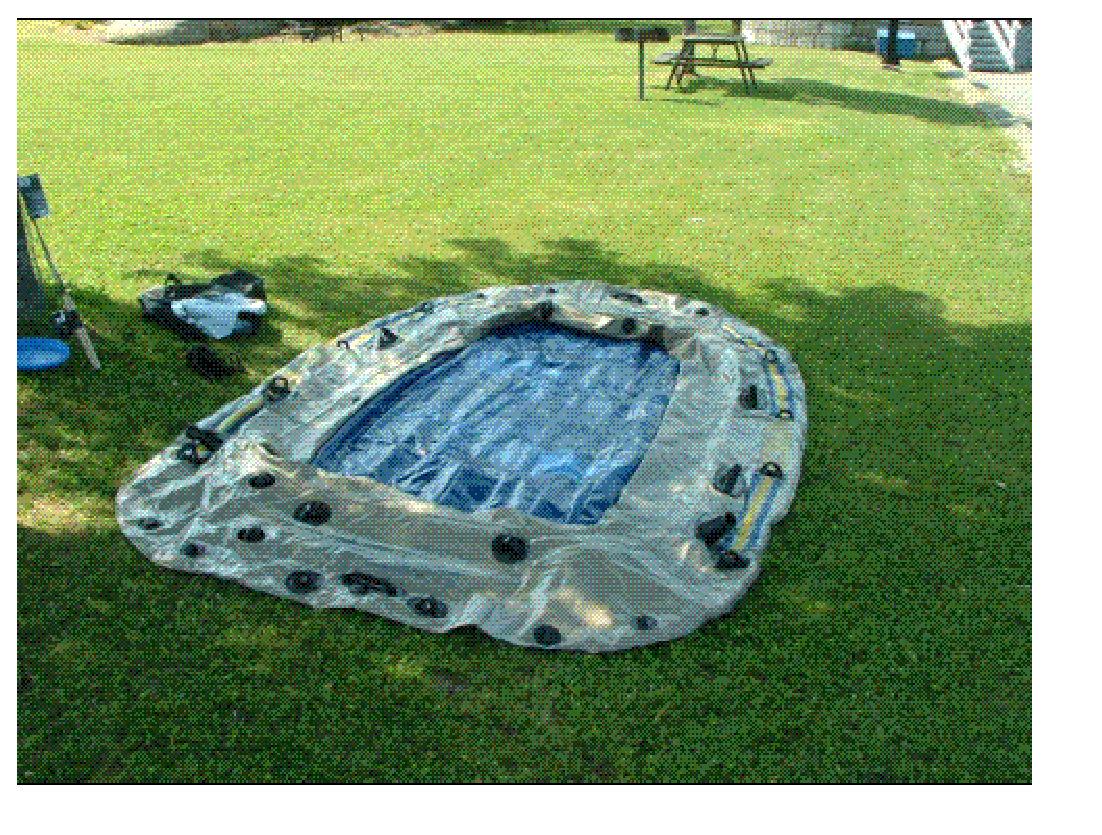
\epsfig{file=fig1.eps,width=3.5in}
Which one of the following is missing in it?
  
  
\noindent\hspace{3.0in} \begin{tabular}{|l|}
\hline
Your choice \\
\hline
 \\ 
 \\ 
\hline
\end{tabular}
  
  
 
 
\noindent{\textbf{\large{
A.}}}
A truck
 
 
\noindent{\textbf{\large{
B.}}}
An air-boat
 
 
\noindent{\textbf{\large{
C.}}}
An airplane
 
 
\noindent{\textbf{\large{
D.}}}
A frisbee
 
 
\noindent{\textbf{\large{
E.}}}
A table
 
 
\noindent{\textbf{\large{
F.}}}
  Not any of aboves.
 
 
 
\vspace{0.3in}
  
\vspace{0.2in}
  
         \begin{tabular}{|l|}
\hline
 Your marks  \\
\hline
 \\ 
 \\ 
\hline
\end{tabular}
\hspace{0.05in} \begin{tabular}{|l|}
\hline
 Full marks  \\
\hline
 \\ 
12.50 \\
\hline
\end{tabular}
{\textbf{\Large{Question
32.1.6 
}}}
  
  
 
An object is subjected to an external net force $\mathbf{f}=(
50.0,  % 
5.0,
-3000.0  )N$. Its mass is known as
$m= % 
54.0 kg$. Please calculate its accelaration.
 
 

 

 
\vspace{0.3in}
   
   
\vspace{0.3in}
{\textbf{\LARGE{You have done all the above? A very good beginning, please go ahead.}}}
More constants the
Mass of electron
$m_e$$ =
9.109390 \times 10^{-31} $
kg
,
Universal gas constant
$R$$ =
8.315 $
J/(mol$\cdot $K)
,
$e$$ =
1.60217733 \times 10^{-19} $
C
, and
$m_p$$ =
1.6726231 \times 10^{-27} $
kg
%
may be very helpful.
\vspace{0.3in}
   
   
  
\vspace{0.2in}
  
\noindent\begin{tabular}{|l|}
\hline
 YOUR MARKS  \\
\hline
 \\ 
 \\ 
\hline
\end{tabular}
\hspace{0.05in} \begin{tabular}{|l|}
\hline
 Full Marks  \\
\hline
 \\ 
1.56 \\
\hline
\end{tabular}
{\textbf{\Large{QUESTION
32.2 
}}}
  
  
If any one of the following statements is correct, please fill the box ahead of it with $T$ .
If wrong, fill with $F$.
 
\noindent\begin{tabular}{|l|l|}\hline Your&\hspace{.2in} \\ answer&\hspace{.2in} \\ \hline \end{tabular}
1. $ % 
5$ is an  % 
odd number.
 
\noindent\begin{tabular}{|l|l|}\hline Your&\hspace{.2in} \\ answer&\hspace{.2in} \\ \hline \end{tabular}
2.  % 
Kingston is in  % 
Ontario province.
 
\noindent\begin{tabular}{|l|l|}\hline Your&\hspace{.2in} \\ answer&\hspace{.2in} \\ \hline \end{tabular}
3.  % 
$\mathbf{F}=m\mathbf{a}$ is a mathmatical form of
the Newton's Second Law.
 

 
\vspace{0.3in}
  
\vspace{0.2in}
  
\noindent\begin{tabular}{|l|}
\hline
 YOUR MARKS  \\
\hline
 \\ 
 \\ 
\hline
\end{tabular}
\hspace{0.05in} \begin{tabular}{|l|}
\hline
 Full Marks  \\
\hline
 \\ 
3.13 \\
\hline
\end{tabular}
{\textbf{\Large{QUESTION
32.3 
}}}
  
  
Considering case-insensitivity, please match the following same strings.
  
  
\begin{tabular}{|l|l|l|}
 \hline
 Column Left & Column Right  & Your choinces \\ 
 \hline
{\textbf{\large{
A.}}}
yjh
  & 
eR
 & 
 \\ 
 \hline
{\textbf{\large{
B.}}}
C
  & 
b
 & 
 \\ 
 \hline
{\textbf{\large{
C.}}}
er
  & 
YJH
 & 
 \\ 
 \hline
{\textbf{\large{
D.}}}
Er
  & 
ER
 & 
 \\ 
 \hline
{\textbf{\large{
E.}}}
B
  & 
c
 & 
 \\ 
 \hline
 \end{tabular}
  
  
 
  
\vspace{0.2in}
  
\noindent\begin{tabular}{|l|}
\hline
 YOUR MARKS  \\
\hline
 \\ 
 \\ 
\hline
\end{tabular}
\hspace{0.05in} \begin{tabular}{|l|}
\hline
 Full Marks  \\
\hline
 \\ 
1.56 \\
\hline
\end{tabular}
{\textbf{\Large{QUESTION
32.4 
}}}
  
  
 
An object is subjected to an external net force $\mathbf{f}=(
20.000 ,
10.0000,
-9000.0  )N$. Its mass is known as
$m= % 
58.0000  kg$. Please choose the correct accelaration
from the following choices.
 
  
  
\noindent\hspace{3.0in} \begin{tabular}{|l|}
\hline
Your choice \\
\hline
 \\ 
 \\ 
\hline
\end{tabular}
  
  
 
 
\noindent{\textbf{\large{
A.}}}
The accelaration is
$(
.99840ms^{-2},
2234.5km/h^2,
-155.17ms^{-2}
).
$
 
 
\noindent{\textbf{\large{
B.}}}
The accelaration is
$(
.34483ms^{-2},
2234.5km/h^2,
-405.11ms^{-2}
).
$
 
 
\noindent{\textbf{\large{
C.}}}
The accelaration is
$(
.34483ms^{-2},
-10755.km/h^2,
-155.17ms^{-2}
).
$
 
 
\noindent{\textbf{\large{
D.}}}
The accelaration is
$(
.99840ms^{-2},
2234.5km/h^2,
-405.11ms^{-2}
).
$
 
 
\noindent{\textbf{\large{
E.}}}
The accelaration is
$(
.34483ms^{-2},
2234.5km/h^2,
-155.17ms^{-2}
).
$
 
 
\noindent{\textbf{\large{
F.}}}
The accelaration is
$(
.99840ms^{-2},
-10755.km/h^2,
-155.17ms^{-2}
).
$
 
 
\noindent{\textbf{\large{
G.}}}
 None of these.
 
 
 
 

 
\vspace{0.3in}
  
\vspace{0.2in}
  
\noindent\begin{tabular}{|l|}
\hline
 YOUR MARKS  \\
\hline
 \\ 
 \\ 
\hline
\end{tabular}
\hspace{0.05in} \begin{tabular}{|l|}
\hline
 Full Marks  \\
\hline
 \\ 
1.56 \\
\hline
\end{tabular}
{\textbf{\Large{QUESTION
32.5 
}}}
  
  
Please choose the correct one from the following statements:
  
  
\noindent\hspace{3.0in} \begin{tabular}{|l|}
\hline
Your choice \\
\hline
 \\ 
 \\ 
\hline
\end{tabular}
  
  
 
 
\noindent{\textbf{\large{
A.}}}
Canada has  %
10 provinces and  %
3 territories.
 
 
\noindent{\textbf{\large{
B.}}}
Canada has  %
37 provinces and  %
37 territories.
 
 
\noindent{\textbf{\large{
C.}}}
Canada has  %
34 provinces and  %
39 territories.
 
 
\noindent{\textbf{\large{
D.}}}
Canada has  %
36 provinces and  %
35 territories.
 
 
\noindent{\textbf{\large{
E.}}}
Canada has  %
35 provinces and  %
34 territories.
 
 
\noindent{\textbf{\large{
F.}}}
 None of above.
 
 
  
\vspace{0.2in}
  
\noindent\begin{tabular}{|l|}
\hline
 YOUR MARKS  \\
\hline
 \\ 
 \\ 
\hline
\end{tabular}
\hspace{0.05in} \begin{tabular}{|l|}
\hline
 Full Marks  \\
\hline
 \\ 
3.13 \\
\hline
\end{tabular}
{\textbf{\Large{QUESTION
32.6 
}}}
  
  
 
 
An object is subjected to an external net force $\mathbf{f}=
(40.0 , 8.0 , -6000.0) N$.
Its mass is known as $m= % 
50.0000 kg$. Please choose the
correct accelaration from the following choices.
 
  
  
\noindent\hspace{3.0in} \begin{tabular}{|l|}
\hline
Your choice \\
\hline
 \\ 
 \\ 
\hline
\end{tabular}
  
  
 
 
\noindent{\textbf{\large{
A.}}}
The accelaration is $  %
(
2.65,
.16,
-120.00)
ms^{-2} $.
 
 
\noindent{\textbf{\large{
B.}}}
The accelaration is $  %
(
.800,
-.64,
-120.00)
ms^{-2} $.
 
 
\noindent{\textbf{\large{
C.}}}
The accelaration is $  %
(
2.65,
-.64,
-120.00)
ms^{-2} $.
 
 
\noindent{\textbf{\large{
D.}}}
The accelaration is $  %
(
2.65,
.16,
-347.33)
ms^{-2} $.
 
 
\noindent{\textbf{\large{
E.}}}
The accelaration is $  %
(
2.65,
-.64,
-347.33)
ms^{-2} $.
 
 
\noindent{\textbf{\large{
F.}}}
The accelaration is $  %
(
.800,
.16,
-120.00)
ms^{-2} $.
 
 
\noindent{\textbf{\large{
G.}}}
The accelaration is $  %
(
.800,
-.64,
-347.33)
ms^{-2} $.
 
 
\noindent{\textbf{\large{
H.}}}
The accelaration is $  %
(
.800,
.16,
-347.33)
ms^{-2} $.
 
 
 

 

 
\vspace{0.3in}
   
   
\vspace{0.3in}
{\textbf{\LARGE{You have done all the above? Excellent! Not much left, please continue.}}}
\vspace{0.3in}
   
   
  
\vspace{0.2in}
  
\noindent\begin{tabular}{|l|}
\hline
 YOUR MARKS  \\
\hline
 \\ 
 \\ 
\hline
\end{tabular}
\hspace{0.05in} \begin{tabular}{|l|}
\hline
 Full Marks  \\
\hline
 \\ 
12.50 \\
\hline
\end{tabular}
{\textbf{\Large{QUESTION
32.7 
}}}
  
  
 
$ \left( \begin{array}{ccccccccc}
           7 & 
           4 & 
           4 & 
           7 \\ 
           6 & 
           4 & 
           5 & 
           7 \\ 
           5 & 
           6 & 
           6 & 
           5
\end{array}\right) \times
\left( \begin{array}{c}
           2 \\ 
           2 \\ 
           2 \\ 
           2
\end{array}\right) $ =?
 
 
$  % 
 \left( \begin{array}
 {
 c
 c
 }
                    \Xi & 
 \eta \\ 
 \Upsilon & 
 \Lambda \\ 
 \delta & 
 \delta \\ 
 \rho & 
 \sigma
 \end{array} \right)
 \left( \begin{array}
 {
 c
 }
 \beta \\ 
 \beta
 \end{array} \right)
$ =?
 

 

 
\vspace{0.3in}
  
\vspace{0.2in}
  
\noindent\begin{tabular}{|l|}
\hline
 YOUR MARKS  \\
\hline
 \\ 
 \\ 
\hline
\end{tabular}
\hspace{0.05in} \begin{tabular}{|l|}
\hline
 Full Marks  \\
\hline
 \\ 
12.50 \\
\hline
\end{tabular}
{\textbf{\Large{QUESTION
32.8 
}}}
  
  
 
An object is subjected to an external net force $\mathbf{f}=
(70.0 , 6.0 , -5000.0) N$.
Its mass is known as $m= % 
58.0 kg$.
Please choose the correct accelaration from the following choices.
  
  
\noindent\hspace{3.0in} \begin{tabular}{|l|}
\hline
Your choice \\
\hline
 \\ 
 \\ 
\hline
\end{tabular}
  
  
 
 
\noindent{\textbf{\large{
A.}}}
  The accelaration is $  %
(
1.21,
.10,
329.96)
ms^{-2} $.
 
 
\noindent{\textbf{\large{
B.}}}
  The accelaration is $  %
(
2.53,
.10,
329.96)
ms^{-2} $.
 
 
\noindent{\textbf{\large{
C.}}}
  The accelaration is $  %
(
2.53,
.49,
329.96)
ms^{-2} $.
 
 
\noindent{\textbf{\large{
D.}}}
  The accelaration is $  %
(
1.21,
.10,
-86.207)
ms^{-2} $.
 
 
 

 
 
\vspace{0.3in}
  
\vspace{0.2in}
  
\noindent\begin{tabular}{|l|}
\hline
 YOUR MARKS  \\
\hline
 \\ 
 \\ 
\hline
\end{tabular}
\hspace{0.05in} \begin{tabular}{|l|}
\hline
 Full Marks  \\
\hline
 \\ 
1.56 \\
\hline
\end{tabular}
{\textbf{\Large{QUESTION
32.9 
}}}
  
  
 
 
% First root
% Second root

 
Please solve the following equation:
\begin{eqnarray*}
1 \times x^2  % 
-2
                 \times x    % 
-15 =0
\end{eqnarray*}
 

 

 
\vspace{0.3in}
   
   
 \vspace{0.2in}
Here are still some constants for use:
 
 
\noindent\begin{tabular}{|l|l|l|}
\hline
Constant & Symbol & Value \\
\hline
 
Mass of proton &
$m_p$ &
 $ 1.6726231 \times 10^{-27} $
kg \\
\hline
 
Boltzmann's constant &
$k$ &
 $ 1.381 \times 10^{-23} $
J/K \\
\hline
 
\end{tabular}
 
Thank you very much for answering these questions!
 
{\textbf{\large{Please be advised}}} that in this paper there are questions from
32.1 through
32.9.
And any one of them may contain more than one sub-question, thus the total number
of sub-questions here is around 14, of which
13 should be answered.
 
   
   
   
   
\vspace{1.0in} 
{\textbf{\large{ *** END OF PAPER, THANKS *** }}} 
   
   
\hspace{1.0in} By: 
         239(         26,          34)
   
   
   
   
\newpage 
\setcounter{page}{ 
    33001 } 
   
   
   
   
\noindent\begin{tabular}{|l|}
\hline
YOUR NAME (FIRST, ... LAST)  \\
\hline
 \\ 
 \\ 
\hline
\end{tabular}
\hspace{0.05in} \begin{tabular}{|l|}
\hline
 YOUR   ID   INFORMATION  \\
\hline
 \\ 
 \\ 
\hline
\end{tabular}
   
   
\vspace{0.2in}\noindent\begin{tabular}{|l|}
\hline
YOUR TOTAL MARKS  \\
\hline
 \\ 
 \\ 
\hline
\end{tabular}
\hspace{0.05in} \begin{tabular}{|l|}
\hline
TOTAL FULL MARKS  \\
\hline
 \\ 
100.00 \\
\hline
\end{tabular}
   
   
 \vspace{0.2in}
 
 
{\Huge  THIS IS AN EXAMPLE OF}
 
{\Huge  PERSONALIZED TESTS. }
 
If needed, please use the following constants.
 
 
 
\noindent\begin{tabular}{|l|l|l|}
\hline
Constant & Symbol & Value \\
\hline
Acceleration due to earth's gravity &
$g$ &
 $ 9.80 $
m/s$^2$ \\
\hline
Avogadro's number &
$N_A$ &
 $ 6.0221367 \times 10^{23} $
mol$^{-1}$ \\
\hline
Boltzmann's constant &
$k$ &
 $ 1.380658 \times 10^{-23} $
J/K \\
\hline
Coulomb's constant &
$k$ &
 $ 8.99 \times 10^{9} $
N$\cdot $m$^2$/C$^2$ \\
\hline
Electron charge magnitiude &
$e$ &
 $ 1.60217733 \times 10^{-19} $
C \\
\hline
Permeability of free space &
$\mu _0$ &
 $ 1.25663706 \times 10^{-6} $
T$\cdot $m/A \\
\hline
Permittivity of free space &
$\epsilon _0$ &
 $ 8.854187817 \times 10^{-12} $
C$^2$/(N$\cdot $m$^2$) \\
\hline
Pi &
$\pi$ &
 $ 3.14159265 $
$ $ \\
\hline
Planck's constant &
$h$ &
 $ 6.6260755 \times 10^{-34} $
J$\cdot $s \\
\hline
Mass of electron &
$m_e$ &
 $ 9.1093897 \times 10^{-31} $
kg \\
\hline
\end{tabular}
 
 
\noindent\begin{tabular}{|l|l|l|}
\hline
Constant & Symbol & Value \\
\hline
Mass of neutron &
$m_n$ &
 $ 1.6749286 \times 10^{-27} $
kg \\
\hline
Mass of proton &
$m_p$ &
 $ 1.6726231 \times 10^{-27} $
kg \\
\hline
Speed of light in vacuum &
$c$ &
 $ 299792458. $
m/s \\
\hline
Universal gravitational constant &
$G$ &
 $ 6.67259 \times 10^{-11} $
N$\cdot $m$^2$/kg$^2$ \\
\hline
Universal gas constant &
$R$ &
 $ 8.314510 $
J/(mol$\cdot $K) \\
\hline
\end{tabular}
 
 
{\textbf{\large{Please be advised}}} that in this paper there are questions from
33.1 through
33.9.
And any one of them may contain more than one sub-question, thus the total number
of sub-questions here is around 14, of which
13 should be answered.
 
\vspace{0.3in}
 
 
   
   
  
\vspace{0.2in}
  
\noindent\begin{tabular}{|l|}
\hline
 YOUR MARKS  \\
\hline
 \\ 
 \\ 
\hline
\end{tabular}
\hspace{0.05in} \begin{tabular}{|l|}
\hline
 Full Marks  \\
\hline
 \\ 
62.50 \\
\hline
\end{tabular}
{\textbf{\Large{QUESTION
33.1 
}}}
  
  
 
{\textbf{\Large{Please answer ONLY
5 of the following
6 questions (Questions
33.1.1 through
33.1.6). }}}
 
Here are still some constants for use in the following questions:
 
 
\noindent\begin{tabular}{|l|l|l|}
\hline
Constant & Symbol & Value \\
\hline
 
Boltzmann's constant &
$k$ &
 $ 1.381 \times 10^{-23} $
J/K \\
\hline
 
Avogadro's number &
$N_A$ &
 $ 6.022 \times 10^{23} $
mol$^{-1}$ \\
\hline
 
Mass of electron &
$m_e$ &
 $ 9.1093897 \times 10^{-31} $
kg \\
\hline
 
\end{tabular}
 
  
\vspace{0.2in}
  
         \begin{tabular}{|l|}
\hline
 Your marks  \\
\hline
 \\ 
 \\ 
\hline
\end{tabular}
\hspace{0.05in} \begin{tabular}{|l|}
\hline
 Full marks  \\
\hline
 \\ 
12.50 \\
\hline
\end{tabular}
{\textbf{\Large{Question
33.1.1 
}}}
  
  
In a hotel, the possiblity of  % 
smoking customer is
$a =  % 
.440$, and the possiblity of  % 
 under 30 years old customer is $ b =  % 
2.00 \times 10^{-2}$.
Please fill the following form.
 
\noindent
\begin{tabular}{|l|l|}
\hline
Customer & Possibility \\
\hline
smoking  and   % 
equal-or-above 30 years old  & \\
\hline
smoking  and   % 
under 30 years old & \\
\hline
 non-smoking and   % 
equal-or-above 30 years old  & \\
\hline
 non-smoking and  % 
under 30 years old & \\
\hline
\end{tabular}
 
 
 

 

 
\vspace{0.3in}
  
\vspace{0.2in}
  
         \begin{tabular}{|l|}
\hline
 Your marks  \\
\hline
 \\ 
 \\ 
\hline
\end{tabular}
\hspace{0.05in} \begin{tabular}{|l|}
\hline
 Full marks  \\
\hline
 \\ 
12.50 \\
\hline
\end{tabular}
{\textbf{\Large{Question
33.1.2 
}}}
  
  
In a hotel, the possiblity of  % 
smoking customer is
$a =  % 
.810$, and the possiblity of  % 
equal or above 30 years old customer is $ b =  % 
.5200$.
Please calculate the possiblity of  % 
 non-smoking and  % 
under 30 years old customer.
 

 

 
\vspace{0.3in}
  
\vspace{0.2in}
  
         \begin{tabular}{|l|}
\hline
 Your marks  \\
\hline
 \\ 
 \\ 
\hline
\end{tabular}
\hspace{0.05in} \begin{tabular}{|l|}
\hline
 Full marks  \\
\hline
 \\ 
12.50 \\
\hline
\end{tabular}
{\textbf{\Large{Question
33.1.3 
}}}
  
  
What is the operation between $a= % 
5$ and $b= % 
2$:
$a$  % 
$\times$ $b=?$ Please also calculate it.

 
\vspace{0.3in}
  
\vspace{0.2in}
  
         \begin{tabular}{|l|}
\hline
 Your marks  \\
\hline
 \\ 
 \\ 
\hline
\end{tabular}
\hspace{0.05in} \begin{tabular}{|l|}
\hline
 Full marks  \\
\hline
 \\ 
12.50 \\
\hline
\end{tabular}
{\textbf{\Large{Question
33.1.4 
}}}
  
  
Let us use Newton's Law of Universal Gravitation to calculate the force
of the Sun acting on the eight planets. Let us suppose the mass of the
Sun is $ % 
2.00 \times 10^{24} kg$. With the mass and the
distance to the Sun of each planet in the following table, please fill
the blanks for the forces.
 
\vspace{0.2in}
 
 
\begin{tabular}{|l|l|l|l|}
\hline
The Planet & Mass ($kg$) & Distanace from Sun ($m$) & The Force ($N$)\\
\hline
Mercury  &
           $ % 
3.00000000 \times 10^{24} $   &
             $ % 
2.000000000 \times 10^{24} $    &
\\  \hline
Venus    &
           $ % 
7.00 \times 10^{24} $    &
             $ % 
5.00 \times 10^{24} $    &
\\  \hline
Earth    &
           $ % 
7.00 \times 10^{24} $    &
             $ % 
9.00 \times 10^{24} $    &
\\   \hline
Mars     &
           $ % 
6.00 \times 10^{24} $    &
             $ % 
5.00 \times 10^{24} $    &
\\   \hline
Jupiter  &
           $ % 
6.00 \times 10^{24} $    &
             $ % 
4.00 \times 10^{24} $    &
\\  \hline
Saturn   &
           $ % 
7.00 \times 10^{24}$    &
             $ % 
7.00 \times 10^{24}$    &
\\  \hline
Uranus   &
           $ % 
8.00 \times 10^{24} $    &
             $ % 
5.00 \times 10^{24} $    &
\\  \hline
Neptune  &
           $ % 
5.00 \times 10^{24} $    &
             $ % 
5.00 \times 10^{24} $    &
\\  \hline
 
\end{tabular}
 
 

 
 

 
\vspace{0.3in}
  
\vspace{0.2in}
  
         \begin{tabular}{|l|}
\hline
 Your marks  \\
\hline
 \\ 
 \\ 
\hline
\end{tabular}
\hspace{0.05in} \begin{tabular}{|l|}
\hline
 Full marks  \\
\hline
 \\ 
12.50 \\
\hline
\end{tabular}
{\textbf{\Large{Question
33.1.5 
}}}
  
  
 
An object is subjected to an external net force $\mathbf{f}=(
70.0 ,
9.0,
-8000.0  )N$. Its mass is known as
$m= % 
50.0  kg$. Please choose the correct accelaration
from the following choices.
 
  
  
\noindent\hspace{3.0in} \begin{tabular}{|l|}
\hline
Your choice \\
\hline
 \\ 
 \\ 
\hline
\end{tabular}
  
  
 
 
\noindent{\textbf{\large{
A.}}}
The accelaration is
$(
1.4000ms^{-2},
.18000ms^{-2},
-5.6351 \times 10^{6}km/h^2
).
$
 
 
\noindent{\textbf{\large{
B.}}}
The accelaration is
$(
1.4000ms^{-2},
.18000ms^{-2},
-2.0736 \times 10^{6}km/h^2
).
$
 
 
\noindent{\textbf{\large{
C.}}}
The accelaration is
$(
3.6739ms^{-2},
-.45089ms^{-2},
-5.6351 \times 10^{6}km/h^2
).
$
 
 
\noindent{\textbf{\large{
D.}}}
The accelaration is
$(
1.4000ms^{-2},
-.45089ms^{-2},
-2.0736 \times 10^{6}km/h^2
).
$
 
 
\noindent{\textbf{\large{
E.}}}
none of these.
 
 
 
 

 
\vspace{0.3in}
  
\vspace{0.2in}
  
         \begin{tabular}{|l|}
\hline
 Your marks  \\
\hline
 \\ 
 \\ 
\hline
\end{tabular}
\hspace{0.05in} \begin{tabular}{|l|}
\hline
 Full marks  \\
\hline
 \\ 
12.50 \\
\hline
\end{tabular}
{\textbf{\Large{Question
33.1.6 
}}}
  
  
See the following picture.
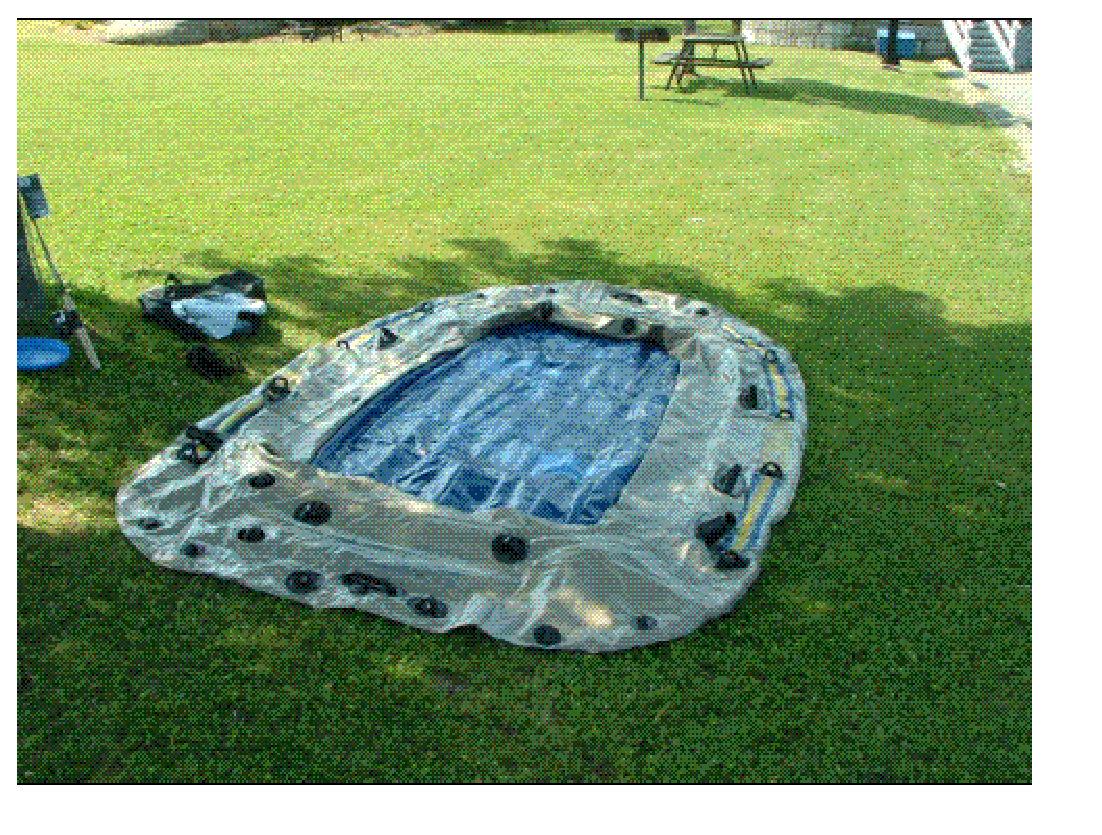
\epsfig{file=fig1.eps,width=3.5in}
Which one of the following is missing in it?
  
  
\noindent\hspace{3.0in} \begin{tabular}{|l|}
\hline
Your choice \\
\hline
 \\ 
 \\ 
\hline
\end{tabular}
  
  
 
 
\noindent{\textbf{\large{
A.}}}
An airplane
 
 
\noindent{\textbf{\large{
B.}}}
A frisbee
 
 
\noindent{\textbf{\large{
C.}}}
Lawn
 
 
\noindent{\textbf{\large{
D.}}}
A table
 
 
\noindent{\textbf{\large{
E.}}}
An air-boat
 
 
\noindent{\textbf{\large{
F.}}}
  Not any of aboves.
 
 
 
\vspace{0.3in}
   
   
\vspace{0.3in}
{\textbf{\LARGE{You have done all the above? A very good beginning, please go ahead.}}}
More constants the
Mass of electron
$m_e$$ =
9.109390 \times 10^{-31} $
kg
,
Universal gas constant
$R$$ =
8.315 $
J/(mol$\cdot $K)
,
$e$$ =
1.60217733 \times 10^{-19} $
C
, and
$m_p$$ =
1.6726231 \times 10^{-27} $
kg
%
may be very helpful.
\vspace{0.3in}
   
   
  
\vspace{0.2in}
  
\noindent\begin{tabular}{|l|}
\hline
 YOUR MARKS  \\
\hline
 \\ 
 \\ 
\hline
\end{tabular}
\hspace{0.05in} \begin{tabular}{|l|}
\hline
 Full Marks  \\
\hline
 \\ 
1.56 \\
\hline
\end{tabular}
{\textbf{\Large{QUESTION
33.2 
}}}
  
  
Please choose the correct one from the following statements:
  
  
\noindent\hspace{3.0in} \begin{tabular}{|l|}
\hline
Your choice \\
\hline
 \\ 
 \\ 
\hline
\end{tabular}
  
  
 
 
\noindent{\textbf{\large{
A.}}}
Canada has  %
10 provinces and  %
3 territories.
 
 
\noindent{\textbf{\large{
B.}}}
Canada has  %
34 provinces and  %
39 territories.
 
 
\noindent{\textbf{\large{
C.}}}
Canada has  %
33 provinces and  %
38 territories.
 
 
\noindent{\textbf{\large{
D.}}}
Canada has  %
35 provinces and  %
34 territories.
 
 
\noindent{\textbf{\large{
E.}}}
Canada has  %
37 provinces and  %
37 territories.
 
 
\noindent{\textbf{\large{
F.}}}
 None of above.
 
 
  
\vspace{0.2in}
  
\noindent\begin{tabular}{|l|}
\hline
 YOUR MARKS  \\
\hline
 \\ 
 \\ 
\hline
\end{tabular}
\hspace{0.05in} \begin{tabular}{|l|}
\hline
 Full Marks  \\
\hline
 \\ 
1.56 \\
\hline
\end{tabular}
{\textbf{\Large{QUESTION
33.3 
}}}
  
  
If any one of the following statements is correct, please fill the box ahead of it with $T$ .
If wrong, fill with $F$.
 
\noindent\begin{tabular}{|l|l|}\hline Your&\hspace{.2in} \\ answer&\hspace{.2in} \\ \hline \end{tabular}
1. $ % 
60$ is an  % 
even number.
 
\noindent\begin{tabular}{|l|l|}\hline Your&\hspace{.2in} \\ answer&\hspace{.2in} \\ \hline \end{tabular}
2.  % 
Kingston is in  % 
Ontario province.
 
\noindent\begin{tabular}{|l|l|}\hline Your&\hspace{.2in} \\ answer&\hspace{.2in} \\ \hline \end{tabular}
3.  % 
$\mathbf{F}=m\mathbf{a}$ is a mathmatical form of
the Newton's Second Law.
 

 
\vspace{0.3in}
  
\vspace{0.2in}
  
\noindent\begin{tabular}{|l|}
\hline
 YOUR MARKS  \\
\hline
 \\ 
 \\ 
\hline
\end{tabular}
\hspace{0.05in} \begin{tabular}{|l|}
\hline
 Full Marks  \\
\hline
 \\ 
3.13 \\
\hline
\end{tabular}
{\textbf{\Large{QUESTION
33.4 
}}}
  
  
 
 
An object is subjected to an external net force $\mathbf{f}=
(20.0 , 9.0 , -4000.0) N$.
Its mass is known as $m= % 
52.0000 kg$. Please choose the
correct accelaration from the following choices.
 
  
  
\noindent\hspace{3.0in} \begin{tabular}{|l|}
\hline
Your choice \\
\hline
 \\ 
 \\ 
\hline
\end{tabular}
  
  
 
 
\noindent{\textbf{\large{
A.}}}
The accelaration is $  %
(
.385,
.17,
-364.54)
ms^{-2} $.
 
 
\noindent{\textbf{\large{
B.}}}
The accelaration is $  %
(
.385,
.60,
-76.923)
ms^{-2} $.
 
 
\noindent{\textbf{\large{
C.}}}
The accelaration is $  %
(
2.64,
.60,
-364.54)
ms^{-2} $.
 
 
\noindent{\textbf{\large{
D.}}}
The accelaration is $  %
(
2.64,
.60,
-76.923)
ms^{-2} $.
 
 
\noindent{\textbf{\large{
E.}}}
The accelaration is $  %
(
2.64,
.17,
-76.923)
ms^{-2} $.
 
 
\noindent{\textbf{\large{
F.}}}
The accelaration is $  %
(
2.64,
.17,
-364.54)
ms^{-2} $.
 
 
\noindent{\textbf{\large{
G.}}}
The accelaration is $  %
(
.385,
.17,
-76.923)
ms^{-2} $.
 
 
\noindent{\textbf{\large{
H.}}}
The accelaration is $  %
(
.385,
.60,
-364.54)
ms^{-2} $.
 
 
 

 

 
\vspace{0.3in}
  
\vspace{0.2in}
  
\noindent\begin{tabular}{|l|}
\hline
 YOUR MARKS  \\
\hline
 \\ 
 \\ 
\hline
\end{tabular}
\hspace{0.05in} \begin{tabular}{|l|}
\hline
 Full Marks  \\
\hline
 \\ 
1.56 \\
\hline
\end{tabular}
{\textbf{\Large{QUESTION
33.5 
}}}
  
  
 
An object is subjected to an external net force $\mathbf{f}=(
100.000 ,
2.0000,
-9000.0  )N$. Its mass is known as
$m= % 
50.0000  kg$. Please choose the correct accelaration
from the following choices.
 
  
  
\noindent\hspace{3.0in} \begin{tabular}{|l|}
\hline
Your choice \\
\hline
 \\ 
 \\ 
\hline
\end{tabular}
  
  
 
 
\noindent{\textbf{\large{
A.}}}
The accelaration is
$(
7.8567ms^{-2},
518.40km/h^2,
720.09ms^{-2}
).
$
 
 
\noindent{\textbf{\large{
B.}}}
The accelaration is
$(
7.8567ms^{-2},
518.40km/h^2,
-180.00ms^{-2}
).
$
 
 
\noindent{\textbf{\large{
C.}}}
The accelaration is
$(
2.0000ms^{-2},
518.40km/h^2,
720.09ms^{-2}
).
$
 
 
\noindent{\textbf{\large{
D.}}}
The accelaration is
$(
2.0000ms^{-2},
1545.6km/h^2,
720.09ms^{-2}
).
$
 
 
\noindent{\textbf{\large{
E.}}}
The accelaration is
$(
2.0000ms^{-2},
1545.6km/h^2,
-180.00ms^{-2}
).
$
 
 
\noindent{\textbf{\large{
F.}}}
The accelaration is
$(
7.8567ms^{-2},
1545.6km/h^2,
-180.00ms^{-2}
).
$
 
 
\noindent{\textbf{\large{
G.}}}
 None of these.
 
 
 
 

 
\vspace{0.3in}
  
\vspace{0.2in}
  
\noindent\begin{tabular}{|l|}
\hline
 YOUR MARKS  \\
\hline
 \\ 
 \\ 
\hline
\end{tabular}
\hspace{0.05in} \begin{tabular}{|l|}
\hline
 Full Marks  \\
\hline
 \\ 
3.13 \\
\hline
\end{tabular}
{\textbf{\Large{QUESTION
33.6 
}}}
  
  
Considering case-insensitivity, please match the following same strings.
  
  
\begin{tabular}{|l|l|l|}
 \hline
 Column Left & Column Right  & Your choinces \\ 
 \hline
{\textbf{\large{
A.}}}
B
  & 
ER
 & 
 \\ 
 \hline
{\textbf{\large{
B.}}}
asdf(:)
  & 
 a= %
2
 & 
 \\ 
 \hline
{\textbf{\large{
C.}}}
er
  & 
YJH
 & 
 \\ 
 \hline
{\textbf{\large{
D.}}}
yjh
  & 
b
 & 
 \\ 
 \hline
{\textbf{\large{
E.}}}
 A= %
4/ %
2

  & 
ASDF(:)
 & 
 \\ 
 \hline
 \end{tabular}
  
  
 
   
   
\vspace{0.3in}
{\textbf{\LARGE{You have done all the above? Excellent! Not much left, please continue.}}}
\vspace{0.3in}
   
   
  
\vspace{0.2in}
  
\noindent\begin{tabular}{|l|}
\hline
 YOUR MARKS  \\
\hline
 \\ 
 \\ 
\hline
\end{tabular}
\hspace{0.05in} \begin{tabular}{|l|}
\hline
 Full Marks  \\
\hline
 \\ 
12.50 \\
\hline
\end{tabular}
{\textbf{\Large{QUESTION
33.7 
}}}
  
  
 
$ \left( \begin{array}{ccccccccc}
           6 & 
           6 & 
           6 & 
           4 \\ 
           5 & 
           4 & 
           5 & 
           6 \\ 
           4 & 
           4 & 
           5 & 
           4
\end{array}\right) \times
\left( \begin{array}{c}
           2 \\ 
           2 \\ 
           2 \\ 
           2
\end{array}\right) $ =?
 
 
$  % 
 \left( \begin{array}
 {
 c
 c
 }
 \Theta & 
 \eta \\ 
 \rho & 
 \Gamma \\ 
                    \zeta & 
 \Delta \\ 
 \alpha & 
 \Theta
 \end{array} \right)
 \left( \begin{array}
 {
 c
 }
 \beta \\ 
 \beta
 \end{array} \right)
$ =?
 

 

 
\vspace{0.3in}
  
\vspace{0.2in}
  
\noindent\begin{tabular}{|l|}
\hline
 YOUR MARKS  \\
\hline
 \\ 
 \\ 
\hline
\end{tabular}
\hspace{0.05in} \begin{tabular}{|l|}
\hline
 Full Marks  \\
\hline
 \\ 
12.50 \\
\hline
\end{tabular}
{\textbf{\Large{QUESTION
33.8 
}}}
  
  
 
An object is subjected to an external net force $\mathbf{f}=
(20.0 , 4.0 , -3000.0) N$.
Its mass is known as $m= % 
54.0 kg$.
Please choose the correct accelaration from the following choices.
  
  
\noindent\hspace{3.0in} \begin{tabular}{|l|}
\hline
Your choice \\
\hline
 \\ 
 \\ 
\hline
\end{tabular}
  
  
 
 
\noindent{\textbf{\large{
A.}}}
  The accelaration is $  %
(
.370,
.16,
187.26)
ms^{-2} $.
 
 
\noindent{\textbf{\large{
B.}}}
  The accelaration is $  %
(
.370,
7.4 \times 10^{-2},
-55.556)
ms^{-2} $.
 
 
\noindent{\textbf{\large{
C.}}}
  The accelaration is $  %
(
1.82,
.16,
187.26)
ms^{-2} $.
 
 
\noindent{\textbf{\large{
D.}}}
  The accelaration is $  %
(
1.82,
7.4 \times 10^{-2},
187.26)
ms^{-2} $.
 
 
 

 
 
\vspace{0.3in}
  
\vspace{0.2in}
  
\noindent\begin{tabular}{|l|}
\hline
 YOUR MARKS  \\
\hline
 \\ 
 \\ 
\hline
\end{tabular}
\hspace{0.05in} \begin{tabular}{|l|}
\hline
 Full Marks  \\
\hline
 \\ 
1.56 \\
\hline
\end{tabular}
{\textbf{\Large{QUESTION
33.9 
}}}
  
  
 
 
% First root
% Second root

 
Please solve the following equation:
\begin{eqnarray*}
3 \times x^2  % 
+  % 
30
                 \times x    % 
-513 =0
\end{eqnarray*}
 

 

 
\vspace{0.3in}
   
   
 \vspace{0.2in}
Here are still some constants for use:
 
 
\noindent\begin{tabular}{|l|l|l|}
\hline
Constant & Symbol & Value \\
\hline
 
Mass of proton &
$m_p$ &
 $ 1.6726231 \times 10^{-27} $
kg \\
\hline
 
Boltzmann's constant &
$k$ &
 $ 1.381 \times 10^{-23} $
J/K \\
\hline
 
\end{tabular}
 
Thank you very much for answering these questions!
 
{\textbf{\large{Please be advised}}} that in this paper there are questions from
33.1 through
33.9.
And any one of them may contain more than one sub-question, thus the total number
of sub-questions here is around 14, of which
13 should be answered.
 
   
   
   
   
\vspace{1.0in} 
{\textbf{\large{ *** END OF PAPER, THANKS *** }}} 
   
   
\hspace{1.0in} By: 
         239(         26,          34)
   
   
   
   
\newpage 
\setcounter{page}{ 
    34001 } 
   
   
   
   
\noindent\begin{tabular}{|l|}
\hline
YOUR NAME (FIRST, ... LAST)  \\
\hline
 \\ 
 \\ 
\hline
\end{tabular}
\hspace{0.05in} \begin{tabular}{|l|}
\hline
 YOUR   ID   INFORMATION  \\
\hline
 \\ 
 \\ 
\hline
\end{tabular}
   
   
\vspace{0.2in}\noindent\begin{tabular}{|l|}
\hline
YOUR TOTAL MARKS  \\
\hline
 \\ 
 \\ 
\hline
\end{tabular}
\hspace{0.05in} \begin{tabular}{|l|}
\hline
TOTAL FULL MARKS  \\
\hline
 \\ 
100.00 \\
\hline
\end{tabular}
   
   
 \vspace{0.2in}
 
 
{\Huge  THIS IS AN EXAMPLE OF}
 
{\Huge  PERSONALIZED TESTS. }
 
If needed, please use the following constants.
 
 
 
\noindent\begin{tabular}{|l|l|l|}
\hline
Constant & Symbol & Value \\
\hline
Acceleration due to earth's gravity &
$g$ &
 $ 9.80 $
m/s$^2$ \\
\hline
Avogadro's number &
$N_A$ &
 $ 6.0221367 \times 10^{23} $
mol$^{-1}$ \\
\hline
Boltzmann's constant &
$k$ &
 $ 1.380658 \times 10^{-23} $
J/K \\
\hline
Coulomb's constant &
$k$ &
 $ 8.99 \times 10^{9} $
N$\cdot $m$^2$/C$^2$ \\
\hline
Electron charge magnitiude &
$e$ &
 $ 1.60217733 \times 10^{-19} $
C \\
\hline
Permeability of free space &
$\mu _0$ &
 $ 1.25663706 \times 10^{-6} $
T$\cdot $m/A \\
\hline
Permittivity of free space &
$\epsilon _0$ &
 $ 8.854187817 \times 10^{-12} $
C$^2$/(N$\cdot $m$^2$) \\
\hline
Pi &
$\pi$ &
 $ 3.14159265 $
$ $ \\
\hline
Planck's constant &
$h$ &
 $ 6.6260755 \times 10^{-34} $
J$\cdot $s \\
\hline
Mass of electron &
$m_e$ &
 $ 9.1093897 \times 10^{-31} $
kg \\
\hline
\end{tabular}
 
 
\noindent\begin{tabular}{|l|l|l|}
\hline
Constant & Symbol & Value \\
\hline
Mass of neutron &
$m_n$ &
 $ 1.6749286 \times 10^{-27} $
kg \\
\hline
Mass of proton &
$m_p$ &
 $ 1.6726231 \times 10^{-27} $
kg \\
\hline
Speed of light in vacuum &
$c$ &
 $ 299792458. $
m/s \\
\hline
Universal gravitational constant &
$G$ &
 $ 6.67259 \times 10^{-11} $
N$\cdot $m$^2$/kg$^2$ \\
\hline
Universal gas constant &
$R$ &
 $ 8.314510 $
J/(mol$\cdot $K) \\
\hline
\end{tabular}
 
 
{\textbf{\large{Please be advised}}} that in this paper there are questions from
34.1 through
34.9.
And any one of them may contain more than one sub-question, thus the total number
of sub-questions here is around 14, of which
13 should be answered.
 
\vspace{0.3in}
 
 
   
   
  
\vspace{0.2in}
  
\noindent\begin{tabular}{|l|}
\hline
 YOUR MARKS  \\
\hline
 \\ 
 \\ 
\hline
\end{tabular}
\hspace{0.05in} \begin{tabular}{|l|}
\hline
 Full Marks  \\
\hline
 \\ 
62.50 \\
\hline
\end{tabular}
{\textbf{\Large{QUESTION
34.1 
}}}
  
  
 
{\textbf{\Large{Please answer ONLY
5 of the following
6 questions (Questions
34.1.1 through
34.1.6). }}}
 
Here are still some constants for use in the following questions:
 
 
\noindent\begin{tabular}{|l|l|l|}
\hline
Constant & Symbol & Value \\
\hline
 
Boltzmann's constant &
$k$ &
 $ 1.381 \times 10^{-23} $
J/K \\
\hline
 
Avogadro's number &
$N_A$ &
 $ 6.022 \times 10^{23} $
mol$^{-1}$ \\
\hline
 
Mass of electron &
$m_e$ &
 $ 9.1093897 \times 10^{-31} $
kg \\
\hline
 
\end{tabular}
 
  
\vspace{0.2in}
  
         \begin{tabular}{|l|}
\hline
 Your marks  \\
\hline
 \\ 
 \\ 
\hline
\end{tabular}
\hspace{0.05in} \begin{tabular}{|l|}
\hline
 Full marks  \\
\hline
 \\ 
12.50 \\
\hline
\end{tabular}
{\textbf{\Large{Question
34.1.1 
}}}
  
  
 
An object is subjected to an external net force $\mathbf{f}=(
70.0 ,
2.0,
-2000.0  )N$. Its mass is known as
$m= % 
52.0  kg$. Please choose the correct accelaration
from the following choices.
 
  
  
\noindent\hspace{3.0in} \begin{tabular}{|l|}
\hline
Your choice \\
\hline
 \\ 
 \\ 
\hline
\end{tabular}
  
  
 
 
\noindent{\textbf{\large{
A.}}}
The accelaration is
$(
6.5126ms^{-2},
3.8462 \times 10^{-2}ms^{-2},
-498462.km/h^2
).
$
 
 
\noindent{\textbf{\large{
B.}}}
The accelaration is
$(
6.5126ms^{-2},
.10556ms^{-2},
1.7228 \times 10^{6}km/h^2
).
$
 
 
\noindent{\textbf{\large{
C.}}}
The accelaration is
$(
1.3462ms^{-2},
3.8462 \times 10^{-2}ms^{-2},
-498462.km/h^2
).
$
 
 
\noindent{\textbf{\large{
D.}}}
The accelaration is
$(
6.5126ms^{-2},
3.8462 \times 10^{-2}ms^{-2},
1.7228 \times 10^{6}km/h^2
).
$
 
 
\noindent{\textbf{\large{
E.}}}
none of these.
 
 
 
 

 
\vspace{0.3in}
  
\vspace{0.2in}
  
         \begin{tabular}{|l|}
\hline
 Your marks  \\
\hline
 \\ 
 \\ 
\hline
\end{tabular}
\hspace{0.05in} \begin{tabular}{|l|}
\hline
 Full marks  \\
\hline
 \\ 
12.50 \\
\hline
\end{tabular}
{\textbf{\Large{Question
34.1.2 
}}}
  
  
Let us use Newton's Law of Universal Gravitation to calculate the force
of the Sun acting on the eight planets. Let us suppose the mass of the
Sun is $ % 
6.00 \times 10^{24} kg$. With the mass and the
distance to the Sun of each planet in the following table, please fill
the blanks for the forces.
 
\vspace{0.2in}
 
 
\begin{tabular}{|l|l|l|l|}
\hline
The Planet & Mass ($kg$) & Distanace from Sun ($m$) & The Force ($N$)\\
\hline
Mercury  &
           $ % 
7.00000000 \times 10^{24} $   &
             $ % 
8.000000000 \times 10^{24} $    &
\\  \hline
Venus    &
           $ % 
4.00 \times 10^{24} $    &
             $ % 
6.00 \times 10^{24} $    &
\\  \hline
Earth    &
           $ % 
5.00 \times 10^{24} $    &
             $ % 
7.00 \times 10^{24} $    &
\\   \hline
Mars     &
           $ % 
6.00 \times 10^{24} $    &
             $ % 
7.00 \times 10^{24} $    &
\\   \hline
Jupiter  &
           $ % 
4.00 \times 10^{24} $    &
             $ % 
4.00 \times 10^{24} $    &
\\  \hline
Saturn   &
           $ % 
4.00 \times 10^{24}$    &
             $ % 
7.00 \times 10^{24}$    &
\\  \hline
Uranus   &
           $ % 
3.00 \times 10^{24} $    &
             $ % 
3.00 \times 10^{24} $    &
\\  \hline
Neptune  &
           $ % 
7.00 \times 10^{24} $    &
             $ % 
3.00 \times 10^{24} $    &
\\  \hline
 
\end{tabular}
 
 

 
 

 
\vspace{0.3in}
  
\vspace{0.2in}
  
         \begin{tabular}{|l|}
\hline
 Your marks  \\
\hline
 \\ 
 \\ 
\hline
\end{tabular}
\hspace{0.05in} \begin{tabular}{|l|}
\hline
 Full marks  \\
\hline
 \\ 
12.50 \\
\hline
\end{tabular}
{\textbf{\Large{Question
34.1.3 
}}}
  
  
 
An object is subjected to an external net force $\mathbf{f}=(
30.0 ,
8.0,
-8000.0  )N$. Its mass is known as
$m= % 
54.0  kg$. Please choose the correct accelaration
from the following choices.
 
  
  
\noindent\hspace{3.0in} \begin{tabular}{|l|}
\hline
Your choice \\
\hline
 \\ 
 \\ 
\hline
\end{tabular}
  
  
 
 
\noindent{\textbf{\large{
A.}}}
The accelaration (vector) is
$(
7200.0,
1920.0 ,
-1.9200 \times 10^{6}
)km/h^2.
$
 
 
\noindent{\textbf{\large{
B.}}}
The accelaration (vector) is
$(
19056.,
1920.0 ,
-8.8002 \times 10^{6}
)km/h^2.
$
 
 
\noindent{\textbf{\large{
C.}}}
The accelaration (vector) is
$(
35393.,
1920.0 ,
-7.4286 \times 10^{6}
)km/h^2.
$
 
 
\noindent{\textbf{\large{
D.}}}
The accelaration (vector) is
$(
33646.,
1920.0 ,
-7.4286 \times 10^{6}
)km/h^2.
$
 
 
\noindent{\textbf{\large{
E.}}}
The accelaration (vector) is
$(
19056.,
1920.0 ,
-7.4286 \times 10^{6}
)km/h^2.
$
 
 
\noindent{\textbf{\large{
F.}}}
The accelaration (vector) is
$(
33646.,
1920.0 ,
6.5973 \times 10^{6}
)km/h^2.
$
 
 
\noindent{\textbf{\large{
G.}}}
The accelaration (vector) is
$(
7200.0,
1920.0 ,
-8.8002 \times 10^{6}
)km/h^2.
$
 
 
\noindent{\textbf{\large{
H.}}}
The accelaration (vector) is
$(
19056.,
1920.0 ,
6.5973 \times 10^{6}
)km/h^2.
$
 
 
\noindent{\textbf{\large{
I.}}}
The accelaration (vector) is
$(
33646.,
1920.0 ,
-1.9200 \times 10^{6}
)km/h^2.
$
 
 
\noindent{\textbf{\large{
J.}}}
The accelaration (vector) is
$(
33646.,
1920.0 ,
-8.8002 \times 10^{6}
)km/h^2.
$
 
 
\noindent{\textbf{\large{
K.}}}
The accelaration (vector) is
$(
7200.0,
1920.0 ,
-7.4286 \times 10^{6}
)km/h^2.
$
 
 
\noindent{\textbf{\large{
L.}}}
The accelaration (vector) is
$(
19056.,
1920.0 ,
-1.9200 \times 10^{6}
)km/h^2.
$
 
 
 
 

 
 
\vspace{0.3in}
  
\vspace{0.2in}
  
         \begin{tabular}{|l|}
\hline
 Your marks  \\
\hline
 \\ 
 \\ 
\hline
\end{tabular}
\hspace{0.05in} \begin{tabular}{|l|}
\hline
 Full marks  \\
\hline
 \\ 
12.50 \\
\hline
\end{tabular}
{\textbf{\Large{Question
34.1.4 
}}}
  
  
In a hotel, the possiblity of  % 
smoking customer is
$a =  % 
.130$, and the possiblity of  % 
 under 30 years old customer is $ b =  % 
.9200$.
Please calculate the possiblity of  % 
 non-smoking and  % 
equal or above 30 years old customer.
 

 

 
\vspace{0.3in}
  
\vspace{0.2in}
  
         \begin{tabular}{|l|}
\hline
 Your marks  \\
\hline
 \\ 
 \\ 
\hline
\end{tabular}
\hspace{0.05in} \begin{tabular}{|l|}
\hline
 Full marks  \\
\hline
 \\ 
12.50 \\
\hline
\end{tabular}
{\textbf{\Large{Question
34.1.5 
}}}
  
  
 
An object is subjected to an external net force $\mathbf{f}=(
20.0,  % 
3.0,
-6000.0  )N$. Its mass is known as
$m= % 
54.0 kg$. Please calculate its accelaration.
 
 

 

 
\vspace{0.3in}
  
\vspace{0.2in}
  
         \begin{tabular}{|l|}
\hline
 Your marks  \\
\hline
 \\ 
 \\ 
\hline
\end{tabular}
\hspace{0.05in} \begin{tabular}{|l|}
\hline
 Full marks  \\
\hline
 \\ 
12.50 \\
\hline
\end{tabular}
{\textbf{\Large{Question
34.1.6 
}}}
  
  
See the following picture.
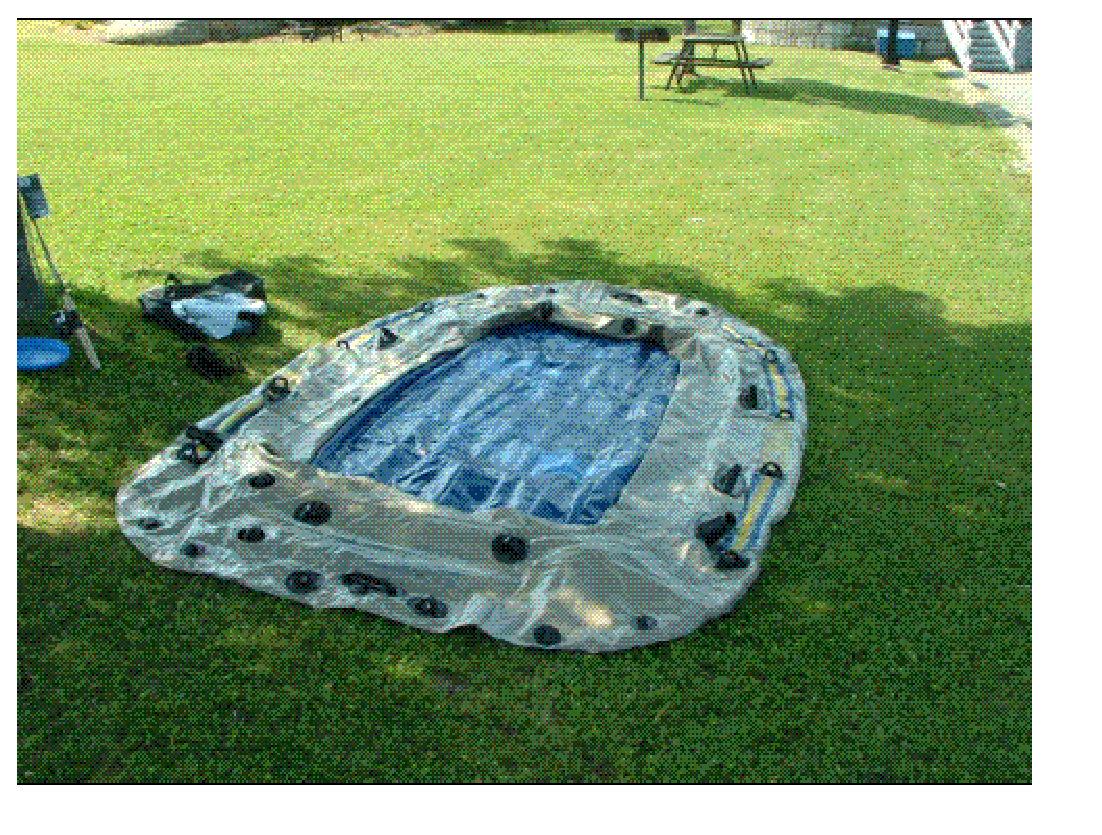
\epsfig{file=fig1.eps,width=3.5in}
Which one of the following is missing in it?
  
  
\noindent\hspace{3.0in} \begin{tabular}{|l|}
\hline
Your choice \\
\hline
 \\ 
 \\ 
\hline
\end{tabular}
  
  
 
 
\noindent{\textbf{\large{
A.}}}
Lawn
 
 
\noindent{\textbf{\large{
B.}}}
An air-boat
 
 
\noindent{\textbf{\large{
C.}}}
A truck
 
 
\noindent{\textbf{\large{
D.}}}
An airplane
 
 
\noindent{\textbf{\large{
E.}}}
A frisbee
 
 
\noindent{\textbf{\large{
F.}}}
  Not any of aboves.
 
 
 
\vspace{0.3in}
   
   
\vspace{0.3in}
{\textbf{\LARGE{You have done all the above? A very good beginning, please go ahead.}}}
More constants the
Mass of electron
$m_e$$ =
9.109390 \times 10^{-31} $
kg
,
Universal gas constant
$R$$ =
8.315 $
J/(mol$\cdot $K)
,
$e$$ =
1.60217733 \times 10^{-19} $
C
, and
$m_p$$ =
1.6726231 \times 10^{-27} $
kg
%
may be very helpful.
\vspace{0.3in}
   
   
  
\vspace{0.2in}
  
\noindent\begin{tabular}{|l|}
\hline
 YOUR MARKS  \\
\hline
 \\ 
 \\ 
\hline
\end{tabular}
\hspace{0.05in} \begin{tabular}{|l|}
\hline
 Full Marks  \\
\hline
 \\ 
1.56 \\
\hline
\end{tabular}
{\textbf{\Large{QUESTION
34.2 
}}}
  
  
 
An object is subjected to an external net force $\mathbf{f}=(
50.000 ,
6.0000,
-5000.0  )N$. Its mass is known as
$m= % 
50.0000  kg$. Please choose the correct accelaration
from the following choices.
 
  
  
\noindent\hspace{3.0in} \begin{tabular}{|l|}
\hline
Your choice \\
\hline
 \\ 
 \\ 
\hline
\end{tabular}
  
  
 
 
\noindent{\textbf{\large{
A.}}}
The accelaration is
$(
1.0000ms^{-2},
1555.2km/h^2,
443.97ms^{-2}
).
$
 
 
\noindent{\textbf{\large{
B.}}}
The accelaration is
$(
2.8752ms^{-2},
7233.3km/h^2,
-100.00ms^{-2}
).
$
 
 
\noindent{\textbf{\large{
C.}}}
The accelaration is
$(
1.0000ms^{-2},
1555.2km/h^2,
-100.00ms^{-2}
).
$
 
 
\noindent{\textbf{\large{
D.}}}
The accelaration is
$(
2.8752ms^{-2},
1555.2km/h^2,
443.97ms^{-2}
).
$
 
 
\noindent{\textbf{\large{
E.}}}
The accelaration is
$(
1.0000ms^{-2},
7233.3km/h^2,
-100.00ms^{-2}
).
$
 
 
\noindent{\textbf{\large{
F.}}}
The accelaration is
$(
2.8752ms^{-2},
1555.2km/h^2,
-100.00ms^{-2}
).
$
 
 
\noindent{\textbf{\large{
G.}}}
 None of these.
 
 
 
 

 
\vspace{0.3in}
  
\vspace{0.2in}
  
\noindent\begin{tabular}{|l|}
\hline
 YOUR MARKS  \\
\hline
 \\ 
 \\ 
\hline
\end{tabular}
\hspace{0.05in} \begin{tabular}{|l|}
\hline
 Full Marks  \\
\hline
 \\ 
3.13 \\
\hline
\end{tabular}
{\textbf{\Large{QUESTION
34.3 
}}}
  
  
 
 
An object is subjected to an external net force $\mathbf{f}=
(40.0 , 10.0 , -8000.0) N$.
Its mass is known as $m= % 
56.0000 kg$. Please choose the
correct accelaration from the following choices.
 
  
  
\noindent\hspace{3.0in} \begin{tabular}{|l|}
\hline
Your choice \\
\hline
 \\ 
 \\ 
\hline
\end{tabular}
  
  
 
 
\noindent{\textbf{\large{
A.}}}
The accelaration is $  %
(
-2.32,
.18,
-545.73)
ms^{-2} $.
 
 
\noindent{\textbf{\large{
B.}}}
The accelaration is $  %
(
.714,
.18,
-545.73)
ms^{-2} $.
 
 
\noindent{\textbf{\large{
C.}}}
The accelaration is $  %
(
.714,
-.68,
-545.73)
ms^{-2} $.
 
 
\noindent{\textbf{\large{
D.}}}
The accelaration is $  %
(
-2.32,
.18,
-142.86)
ms^{-2} $.
 
 
\noindent{\textbf{\large{
E.}}}
The accelaration is $  %
(
-2.32,
-.68,
-545.73)
ms^{-2} $.
 
 
\noindent{\textbf{\large{
F.}}}
The accelaration is $  %
(
-2.32,
-.68,
-142.86)
ms^{-2} $.
 
 
\noindent{\textbf{\large{
G.}}}
The accelaration is $  %
(
.714,
.18,
-142.86)
ms^{-2} $.
 
 
\noindent{\textbf{\large{
H.}}}
The accelaration is $  %
(
.714,
-.68,
-142.86)
ms^{-2} $.
 
 
 

 

 
\vspace{0.3in}
  
\vspace{0.2in}
  
\noindent\begin{tabular}{|l|}
\hline
 YOUR MARKS  \\
\hline
 \\ 
 \\ 
\hline
\end{tabular}
\hspace{0.05in} \begin{tabular}{|l|}
\hline
 Full Marks  \\
\hline
 \\ 
1.56 \\
\hline
\end{tabular}
{\textbf{\Large{QUESTION
34.4 
}}}
  
  
Please choose the correct one from the following statements:
  
  
\noindent\hspace{3.0in} \begin{tabular}{|l|}
\hline
Your choice \\
\hline
 \\ 
 \\ 
\hline
\end{tabular}
  
  
 
 
\noindent{\textbf{\large{
A.}}}
Canada has  %
36 provinces and  %
35 territories.
 
 
\noindent{\textbf{\large{
B.}}}
Canada has  %
34 provinces and  %
39 territories.
 
 
\noindent{\textbf{\large{
C.}}}
Canada has  %
37 provinces and  %
37 territories.
 
 
\noindent{\textbf{\large{
D.}}}
Canada has  %
33 provinces and  %
38 territories.
 
 
\noindent{\textbf{\large{
E.}}}
Canada has  %
10 provinces and  %
3 territories.
 
 
\noindent{\textbf{\large{
F.}}}
 None of above.
 
 
  
\vspace{0.2in}
  
\noindent\begin{tabular}{|l|}
\hline
 YOUR MARKS  \\
\hline
 \\ 
 \\ 
\hline
\end{tabular}
\hspace{0.05in} \begin{tabular}{|l|}
\hline
 Full Marks  \\
\hline
 \\ 
1.56 \\
\hline
\end{tabular}
{\textbf{\Large{QUESTION
34.5 
}}}
  
  
If any one of the following statements is correct, please fill the box ahead of it with $T$ .
If wrong, fill with $F$.
 
\noindent\begin{tabular}{|l|l|}\hline Your&\hspace{.2in} \\ answer&\hspace{.2in} \\ \hline \end{tabular}
1. $ % 
97$ is an  % 
odd number.
 
\noindent\begin{tabular}{|l|l|}\hline Your&\hspace{.2in} \\ answer&\hspace{.2in} \\ \hline \end{tabular}
2.  % 
Kingston is in  % 
Ontario province.
 
\noindent\begin{tabular}{|l|l|}\hline Your&\hspace{.2in} \\ answer&\hspace{.2in} \\ \hline \end{tabular}
3.  % 
$\mathbf{F}=m\mathbf{a}$ is a mathmatical form of
the Newton's Second Law.
 

 
\vspace{0.3in}
  
\vspace{0.2in}
  
\noindent\begin{tabular}{|l|}
\hline
 YOUR MARKS  \\
\hline
 \\ 
 \\ 
\hline
\end{tabular}
\hspace{0.05in} \begin{tabular}{|l|}
\hline
 Full Marks  \\
\hline
 \\ 
3.13 \\
\hline
\end{tabular}
{\textbf{\Large{QUESTION
34.6 
}}}
  
  
Considering case-insensitivity, please match the following same strings.
  
  
\begin{tabular}{|l|l|l|}
 \hline
 Column Left & Column Right  & Your choinces \\ 
 \hline
{\textbf{\large{
A.}}}
C
  & 
YJH
 & 
 \\ 
 \hline
{\textbf{\large{
B.}}}
A
  & 
a
 & 
 \\ 
 \hline
{\textbf{\large{
C.}}}
B
  & 
c
 & 
 \\ 
 \hline
{\textbf{\large{
D.}}}
asdf(:)
  & 
ASDF(:)
 & 
 \\ 
 \hline
{\textbf{\large{
E.}}}
yjh
  & 
b
 & 
 \\ 
 \hline
 \end{tabular}
  
  
 
   
   
\vspace{0.3in}
{\textbf{\LARGE{You have done all the above? Excellent! Not much left, please continue.}}}
\vspace{0.3in}
   
   
  
\vspace{0.2in}
  
\noindent\begin{tabular}{|l|}
\hline
 YOUR MARKS  \\
\hline
 \\ 
 \\ 
\hline
\end{tabular}
\hspace{0.05in} \begin{tabular}{|l|}
\hline
 Full Marks  \\
\hline
 \\ 
12.50 \\
\hline
\end{tabular}
{\textbf{\Large{QUESTION
34.7 
}}}
  
  
 
$ \left( \begin{array}{ccccccccc}
           5 & 
           5 & 
           4 & 
           6 \\ 
           6 & 
           4 & 
           7 & 
           5 \\ 
           7 & 
           7 & 
           7 & 
           7
\end{array}\right) \times
\left( \begin{array}{c}
           2 \\ 
           2 \\ 
           2 \\ 
           2
\end{array}\right) $ =?
 
 
$  % 
 \left( \begin{array}
 {
 c
 c
 }
                    \zeta & 
 \varepsilon \\ 
 \gamma & 
 \Gamma \\ 
 \Theta & 
 \varepsilon \\ 
 \gamma & 
                    \zeta
 \end{array} \right)
 \left( \begin{array}
 {
 c
 }
 \beta \\ 
 \beta
 \end{array} \right)
$ =?
 

 

 
\vspace{0.3in}
  
\vspace{0.2in}
  
\noindent\begin{tabular}{|l|}
\hline
 YOUR MARKS  \\
\hline
 \\ 
 \\ 
\hline
\end{tabular}
\hspace{0.05in} \begin{tabular}{|l|}
\hline
 Full Marks  \\
\hline
 \\ 
12.50 \\
\hline
\end{tabular}
{\textbf{\Large{QUESTION
34.8 
}}}
  
  
 
An object is subjected to an external net force $\mathbf{f}=
(90.0 , 9.0 , -4000.0) N$.
Its mass is known as $m= % 
54.0 kg$.
Please choose the correct accelaration from the following choices.
  
  
\noindent\hspace{3.0in} \begin{tabular}{|l|}
\hline
Your choice \\
\hline
 \\ 
 \\ 
\hline
\end{tabular}
  
  
 
 
\noindent{\textbf{\large{
A.}}}
  The accelaration is $  %
(
1.67,
.17,
264.68)
ms^{-2} $.
 
 
\noindent{\textbf{\large{
B.}}}
  The accelaration is $  %
(
1.67,
-.50,
-74.074)
ms^{-2} $.
 
 
\noindent{\textbf{\large{
C.}}}
  The accelaration is $  %
(
1.67,
.17,
-74.074)
ms^{-2} $.
 
 
\noindent{\textbf{\large{
D.}}}
  The accelaration is $  %
(
7.96,
.17,
264.68)
ms^{-2} $.
 
 
 

 
 
\vspace{0.3in}
  
\vspace{0.2in}
  
\noindent\begin{tabular}{|l|}
\hline
 YOUR MARKS  \\
\hline
 \\ 
 \\ 
\hline
\end{tabular}
\hspace{0.05in} \begin{tabular}{|l|}
\hline
 Full Marks  \\
\hline
 \\ 
1.56 \\
\hline
\end{tabular}
{\textbf{\Large{QUESTION
34.9 
}}}
  
  
 
 
% First root
% Second root

 
Please solve the following equation:
\begin{eqnarray*}
-5 \times x^2  % 
+  % 
205
                 \times x    % 
-2100 =0
\end{eqnarray*}
 

 

 
\vspace{0.3in}
   
   
 \vspace{0.2in}
Here are still some constants for use:
 
 
\noindent\begin{tabular}{|l|l|l|}
\hline
Constant & Symbol & Value \\
\hline
 
Mass of proton &
$m_p$ &
 $ 1.6726231 \times 10^{-27} $
kg \\
\hline
 
Boltzmann's constant &
$k$ &
 $ 1.381 \times 10^{-23} $
J/K \\
\hline
 
\end{tabular}
 
Thank you very much for answering these questions!
 
{\textbf{\large{Please be advised}}} that in this paper there are questions from
34.1 through
34.9.
And any one of them may contain more than one sub-question, thus the total number
of sub-questions here is around 14, of which
13 should be answered.
 
   
   
   
   
\vspace{1.0in} 
{\textbf{\large{ *** END OF PAPER, THANKS *** }}} 
   
   
\hspace{1.0in} By: 
         239(         26,          34)
   
   
 
 
\end{document}
